\documentclass[12pt]{myucthesis}

%\nofiles
% The above command prevents latex from writing its auxiliary
% files. This is useful if you want to manually tweak them before you
% generate your final PDF.


% Page layout. The fancyhdr package may complain about the need for a
% larger headheight, depending on how long chapter titles are; if left
% unspecified in the geometry setup, it defaults to 12pt. The
% "showframe" option causes the geometry package (version >= 5.0) to
% show a frame around the margins on every page, which is great for
% checking that you don't overflow anywhere.

%\usepackage[letterpaper,includehead,margin=1in,headheight=15pt,showframe]{geometry}
\usepackage[letterpaper,includehead,margin=1in,headheight=15pt]{geometry}
\usepackage{fancyhdr}
\pagestyle{fancyplain}
\lhead[\fancyplain{\thepage}{\thepage}]{\fancyplain{}{\scshape\rightmark}}
\rhead[\fancyplain{}{\scshape\leftmark}]{\fancyplain{\thepage}{\thepage}}
\chead{}
\cfoot{}
\lfoot{}
\rfoot{}


% Bibliography stuff:

\newcommand{\newblock}{\par} % need this for some natbib internal bug
\usepackage{natbib}
\citestyle{aa}
\bibliographystyle{yahapj}
\setlength{\bibsep}{0ex} % single-space entries
\def\bibpreamble{\addcontentsline{toc}{chapter}{Bibliography}} % get a good TOC entry


% Other setup:

\usepackage[T1]{fontenc} % see http://tinyurl.com/67zdxwf
\usepackage[colorlinks,urlcolor=blue,citecolor=blue,linkcolor=blue,pdfusetitle]{hyperref}
\usepackage{pdflscape} % allows landscape-oriented figures with PDF page rotation
\usepackage{aasmacros,amsmath,amssymb,graphicx}
\usepackage{mydeluxetable} % deluxetable customized to play well with ucthesis


\begin{document}
\ssp % single spacing
\hypersetup{pageanchor=false}
\title{Galaxies and Dark Matter in Groups}
\author{Matthew Richard George} % must match BearFacts!
\degreesemester{Fall}
\degreeyear{2014}
\degree{Doctor of Philosophy}
\numberofmembers{4}
\chair{David Schlegel}
\othermembers{
Uros Seljak \\
Marc Davis \\
Saul Perlmutter
}
\field{Astrophysics}
\campus{Berkeley}

\maketitle
\copyrightpage

\begin{abstract}
Thesis abstract goes here.
\end{abstract}

\hypersetup{pageanchor=true}
\begin{frontmatter}

%\begin{dedication}
%\null\vfil
%{\large
%\begin{center}
%I dedicate this dissertation to graduate students everywhere.
%\end{center}}
%\null\vfil
%\end{dedication}

\tableofcontents
\listoffigures % optional
\listoftables % optional

% If using code.sty, can also add:
%% \listofcodes
%% \addcontentsline{toc}{chapter}{List of Code Examples}

\begin{acknowledgements}
Thesis acknowledgements go here.

% Feel free to modify or remove this acknowledgment:
This dissertation was typeset using the
\href{https://github.com/pkgw/ucastrothesis}{\textsf{ucastrothesis}}
\LaTeX\ template.

\end{acknowledgements}
\end{frontmatter}

\chapter{Introduction}
\label{chap:intro}

%\begin{quote}{\textit{``A thesis is not supposed to be your best work; it's just
%  practice.''}
%
%--- Marc Davis}
%\end{quote}

A multitude of observations of our Universe, from the anisotropies of
the cosmic microwave background to the clustering of galaxies and the
expansion history derived from supernovae, can be described by a
simple yet befuddling cosmological model. In this model the familiar
baryonic component of the Universe, which can be detected through
electromagnetic interactions, is dwarfed by two dark constituents that
dominate the energy density. Dark matter is effectively collisionless
and nonrelativistic, seeding structure growth and hosting galaxies in
deep gravitational potentials called halos. Perturbations in the
density of baryons and dark matter, initialized after a period of
rapid inflation, eventually collapsed under gravitational instability
to form these galaxies and halos which merge and grow
hierarchically. Dark energy exerts a uniform negative pressure,
accelerating expansion and suppressing structure growth at late
times. The existence of these dark components implies that extensions
are necessary to our standard models of particle physics, gravity, or
both.

Testing the validity of this cosmological model and constraining its
parameters is the focus of much observational and theoretical effort.
What is dark matter and how is it distributed in space?  Does it
couple with baryons or self-interact in detectable ways?  Does the
dark energy density vary with space or time? Does general
relativity accurately describe gravity on large and small scales?
These are the questions we ultimately aim to address to further our
understanding of the dark side of our Universe.

On large scales, the distribution of matter is accurately described by
the linear evolution of density perturbations from inflation under
gravitational instability. On smaller scales, density fluctuations
become nonlinear and collapse into halos. Halos are densest near their
centers and may host a central galaxy, and more massive halos can host
additional satellite galaxies that sample the dark matter
density as a stochastic tracer. Numerical simulations reveal a wide
variety of halo shapes and density profiles for these halos, but on
average they are spherical and can be described with a simple model
the depends on their mass and concentration. A halo model with these
assumptions can remarkably reproduce many observations of
nonlinear structure.

There is still much to be learned from constraining the parameters of
this cosmological model and determining where the simplifying
description of halos breaks down. The growth of structure can be
measured from the distribution of halo masses and its evolution over
time. This offers a test of dark energy that is complementary to
measurements of the expansion history.  The detailed density profiles
in halos and abundance of substructure are sensitive to the mass and
interaction cross section of dark matter, which ultimately tell us
about the physics of its formation.

Complications arise when constraining these quantities from
observations. Galaxy surveys have served as the workhorse for
large-scale structure measurements. Wide area imaging taken at Lick
Observatory in the 1950s provided the first systematic probe of the
large-scale spatial distribution of galaxies. Later the CfA Redshift
Survey added a third dimension to such maps, and opened the field for
a proliferation of modern experiments including the Sloan Digital Sky
Survey and DEEP2, pushing boundaries in volume and depth of
coverage. Multi-wavelength imaging and spectroscopic surveys such as
COSMOS have supplemented these optical studies with observations
from radio to X-ray bands, providing new insight into the interplay of
stars and gas with dark matter.

Dark matter halo masses and density profiles can only be measured from
these data indirectly. Galaxies are visible tracers of the dark matter
density field, but the details of how galaxies populate dark matter
halos can be complicated. From two- or three-dimensional maps, groups
and clusters of galaxies can be identified based on their
proximity. Many estimators have been employed to extract halo masses
from observables. Galaxy counts, luminosities, and stellar masses can
be derived relatively inexpensively, while it is generally more costly
to measure galaxy dynamics or the temperature and luminosity profiles
of the hot gas in massive halos. Gravitational lensing offers another
probe of the projected matter distribution that is in principle
independent of the baryonic tracers used in other estimators. In
general, these methods have been shown to correlate with one another
and produce a coherent picture of halo masses and density profiles.
But for precision cosmology, it is essential to probe these small
nonlinear scales and to improve our understanding of the biases in
techniques for extracting the matter distribution from observations.

The mission to understand how galaxies trace dark matter plays in
important role in cosmological studies, but also raises interesting
questions in its own right. Galaxy properties are broadly bimodal,
with a population of more massive and luminous red galaxies that tend
to have older stellar populations, more spheroidal morphologies, and
concentrated light profiles than a distinct population of younger,
blue star-forming galaxies. Why do galaxies look the way they do, and
what processes led to the menagerie we observe?

This thesis presents a systematic study of the relationships between
galaxy properties and their environment, to both address the basic
questions about galaxy evolution and to support further cosmological
study with a better understanding of how galaxies inhabit dark matter
halos. I have connected measurements of X-ray emission and weak
lensing for a large sample of galaxy groups spanning nearly half the
age of the Universe \citep{George2011}. This sample consists of the
most massive halos in the largest contiguous area mapped by the Hubble
Space Telescope, and and includes new optical spectroscopy of group
members. This group sample has been exploited with the high-resolution
imaging and multi-wavelength photometry from the COSMOS survey to
constrain dark matter halo properties of this group sample with weak
lensing \citep{Leauthaud2010, George2012, Schmidt2012, Ford2012,
  Taylor2012} and also for studying the masses, colors, and
morphologies of galaxies residing in these halos \citep{George2011,
  George2013, Leauthaud2012b}.  Miscentering is a dominant systematic
uncertainty in measuring halo masses \citep{Rozo2011}, so identifying
correct centers and modeling offsets is crucial. To address this
issue, I developed a new approach to find halo centers based on the
stacked weak lensing signal \citep{George2012}. The models I developed
can readily be extended to measure substructure around satellites and
the stellar mass to light ratio in galaxies with lensing and dynamical
measurements.

The properties of galaxies are linked to their environment, and
quantifying these correlations is important to understand the
coevolution of baryonic and dark matter. While it has long been known
that dense environments host galaxies with greater masses, lower
star-formation rates, and more bulge-dominated morphologies
\citep[see][for a review]{Blanton2009}, the processes that produce these
correlations remain unclear, in part due to the many interrelated
variables at play. Large data sets from recent and upcoming surveys
are finally enabling us to isolate trends in specific properties with
others fixed. This study of group member galaxies quantifies
the separate dependences of galaxy color and morphology on
group-centric distance (at effectively fixed stellar mass, halo mass,
and redshift), which constrains models of galaxy evolution involving
gas stripping, feedback, and mergers \citep{George2013}.

The work in this thesis has been published in three separate papers,
each of which is translated into a chapter
here. Chapter~\ref{chap:catalog} \citep{George2011} describes the
construction of the group catalog and detailed tests of group
membership assignment using simulations. Chapter~\ref{chap:centering}
\citep{George2012} presents a weak lensing study to test different
tracers of halo centers and their impact on halo mass
estimates. Chapter~\ref{chap:transformers} \citep{George2013} employs
those halo centers to measure the dependence of galaxy properties on
groupcentric distance, illustrating how star-formation rates and
structural parameters in galaxies are related to the dark matter halos
they inhabit.
%Chapter~\ref{chap:outlook} - outlook beyond continuing similar
%analyses with new surveys; new techniques for mapping dark matter
%(spectroscopic lensing and peculiar velocities).

%-------- MACROS ------------
 \newcommand{\eg}{{e.g.}}
 \newcommand{\cf}{{c.f.}}
 \newcommand{\ie}{{i.e.}}
 \newcommand{\etc}{{etc.}}
 \newcommand{\sn}{S{\rm /}N}
 \newcommand{\rmd}{{\rm d}}
 \newcommand{\Msol}{\mbox{$M_{\odot}$}}
 \newcommand{\msun}{\mbox{$M_{\odot}$}}
 \newcommand{\Msun}{\mbox{${\bf M_{\odot} }$}}
 \newcommand{\Lsol}{\mbox{$L_{\odot}$}}
 \newcommand{\lsun}{\mbox{$L_{\odot}$}}
 \newcommand{\ergsec}{\mbox{erg s$^{-1}$}}
 \newcommand{\rvir}{\mbox{$R_{200\rm{c}}$}}
 \newcommand{\mvir}{\mbox{$M_{200\rm{c}}$}}
\newcommand{\zp}{\mbox{$z_{\rm p}$}}
 \newcommand{\zs}{\mbox{$z_{\rm s}$}}
\newcommand{\zG}{\mbox{$z_{\rm G}$}}
\newcommand{\pz}{\mbox{$\mathcal{P}(z)$}}
\newcommand{\flux}{erg cm$^{-2}$ s$^{-1}$ }
\newcommand{\nuvr}{{$(\rm{NUV} - r^+)$ }}

\chapter{Galaxies in X-ray Groups I: 
Robust Membership Assignment and 
the Impact of Group Environments on Quenching}

\label{chap:catalog}

%-------- ABSTRACT  ---------------------
Understanding the mechanisms that lead dense environments to host
galaxies with redder colors, more spheroidal morphologies, and lower
star formation rates than field populations remains an important
problem. As most candidate processes ultimately depend on host halo
mass, accurate characterizations of the local environment, ideally
tied to halo mass estimates and spanning a range in halo mass and
redshift are needed.  In this work, we present and test a rigorous,
probabalistic method for assigning galaxies to groups based on precise
photometric redshifts and X-ray selected groups drawn from the COSMOS
field.  The groups have masses in the range $10^{13} \lesssim
M_{200\rm{c}}/M_{\odot} \lesssim 10^{14}$ and span redshifts
$0<z<1$. We characterize our selection algorithm via tests on
spectroscopic subsamples, including new data obtained at the VLT, and
by applying our method to detailed mock catalogs.  We find 
that our group member galaxy sample has a purity of $84\%$ and
completeness of $92\%$ within $0.5\rvir$. We measure the impact of
uncertainties in redshifts and group centering on the quality of the
member selection with simulations based on current data as well as
future imaging and spectroscopic surveys. As a first application of
our new group member catalog which will be made publicly available, we
show that member galaxies exhibit a higher quenched fraction compared
to the field at fixed stellar mass out to $z \sim 1$, indicating a
significant relationship between star formation and environment at
group scales.  We also address the suggestion that dusty star forming
galaxies in such groups may impact the high-$\ell$ power spectrum of
the cosmic microwave background and find that such a population cannot
explain the low power seen in recent SZ measurements. 
 

\section{Introduction}
\setcounter{footnote}{0}

Galaxies in dense cluster regions have long been known to have
different characteristics than counterparts in the field, with redder colors,
a greater tendency for spheroidal morphologies, and suppressed star
formation rates. Dense clusters are also the sites of the most massive
and luminous galaxies. Much effort has been made to find the redshift, halo
mass, and cluster-centric distance at which these distinctions between
galaxy populations are imprinted and the process by which these
transformations occur \citep[e.g.,][]{Oemler1974, Dressler1980, Butcher1984, Dressler1997,
Poggianti1999, Lewis2002, Goto2003, Balogh2004, DePropris2004,
Kauffmann2004, Lin2004a, Blanton2005, Cucciati2006, Cooper2006, Weinmann2006, Capak2007a,
Gerke2007, Blanton2009, Hansen2009, Mei2009, Feruglio2010}.
While massive clusters present clear
examples of galaxy transformations due to gas stripping, merger
activity, and tidal disruption \citep[e.g.,][]{Kenney1995,
  Gavazzi2001, Cortese2007}, the extent to which these
processes  
affect the majority of galaxies which live in less dense environments
is uncertain. Extending cluster samples to groups with lower halo
masses and higher redshifts is challenging because it requires
significant observational expenditures and careful analysis to isolate
such environments from the field. 

Recent analyses at low redshift have confirmed the existence of an
environmental dependence of galactic structure and colors across a
range of environments \citep[e.g.,][]{Kauffmann2004, Baldry2006,
  Bamford2009}. The corresponding picture at $z\sim1$ has been less clear. With
pointed observations around high-redshift galaxy clusters, several
studies have found significant trends in morphology, color, and
star-formation rate with local galaxy density
\citep[e.g.,][]{Postman2005, Smith2005a, Tanaka2005, Poggianti2008}.
However, some find that the relations disappear in stellar mass-selected
samples, arguing that environmental trends are due to differences in
the stellar mass distribution between environments rather than
physical processes acting in dense regions
\citep[e.g.,][]{Poggianti2008}. 

In field surveys reaching $z\sim1$, results from
the VIRMOS-VLT Deep Survey \citep[VVDS;][]{Scodeggio2009} and zCOSMOS
\citep{Tasca2009,  Cucciati2010, Iovino2010, Kovac2010b} show little or
no environmental influence on morphology and color especially at high
stellar masses ($\log(M_{\star}/M_{\odot})\gtrsim10.7$), while results
from DEEP2 \citep{Cooper2010} and others from zCOSMOS \citep{Peng2010}
show a clear relationship between color and environment. These papers
generally find weakening environmental trends with increasing
redshift, but differ in the redshift at which the trends
disappear. \citet{Cooper2007} and \citet{Cooper2010} discuss the discrepancies in
environmental trends seen in high-redshift field surveys and suggest
that the non-detection by some studies could be due to
the use of less confident spectroscopic redshifts and lower sampling rates, as
well as increased difficulty with determining environmental densities
using optical spectroscopy at high redshift, while \citet{Peng2010}
attributes the differences to the definitions used to characterize
environments.

The aim of this work is to define a clean sample of galaxies in dense
group environments out to redshift $z=1$ to address these issues. We study groups from the
COSMOS survey that have been identified as sources of extended X-ray
emission \citep[][and in prep.]{Finoguenov2007}, which is a strong
indication that they are virialized structures and not chance
associations of galaxies. The groups have halo masses in the range
$10^{13} \lesssim M_{200\rm{c}}/M_{\odot} \lesssim 10^{14}$ as
determined by weak lensing \citep{Leauthaud2010}.  In a companion
paper, we describe weak lensing tests to optimize the identification
of halo centers (Paper II; George et al., in prep.). We select member
galaxies based on photometric redshifts derived from
extensive multi-wavelength imaging, which provides a
much greater sampling density than existing spectroscopic
surveys. Using a spectroscopic subsample and mock catalogs, we
carefully evaluate our member selection for potential biases or
contamination, and account for photometric redshift
uncertainties. This robust sample of group members can be used to
address unsettled questions about the link between galaxies and their
environments.

A key challenge is to disentangle the intrinsic and extrinsic factors
that may play a role in shaping galaxy properties. For instance, galaxies
in dense regions have a higher characteristic stellar mass than in
less dense environments \citep[e.g.,][]{Baldry2006}, so a
morphology-mass relation could be conflated with a morphology-density
relation. Since stellar mass plays an important role in determining
galaxy properties, and mass-to-light ratios are strongly affected by
star formation activity, recent environmental studies have stressed
the use of stellar mass-selected samples rather than
luminosity-selected samples to make a fair comparison across
environments \citep[e.g.,][]{VanDerWel2007, Scodeggio2009,
  Cooper2010}.

In addition to controlling for intrinsic galaxy
properties in these studies, defining and measuring the
``environment'' presents another problem. The distance to the $N$th
nearest neighbor or the mean density of galaxies inside a fixed radius
are commonly used as environmental indicators
\citep[e.g.,][]{Dressler1980}. \citet{Kauffmann2004}
show that galaxy properties correlate most tightly with
local density on scales below $\sim1~\rm{Mpc}$ and are uncorrelated
with the density on larger scales once the small-scale density is
fixed. Several studies have shown evidence
that galaxy properties correlate most tightly with density within
their halo, and have emphasized that the aperture used for comparing
equivalent regions must scale with halo mass to avoid confusion
between local and global densities \citep{Hansen2005, Weinmann2006,
  Blanton2007, Haas2011}. Instead of using the galaxy density field to
define environment, one can define a catalog of galaxy groups and
clusters and study their properties as a function of halo mass and
group-centric distance. In this paper we use the term ``group'' to
denote a set of galaxies with a common dark matter halo and to
emphasize the low mass range studied, making no formal distinction
between groups and clusters.

Catalogs of galaxy groups have been constructed from both optical
surveys identifying galaxy overdensities and X-ray surveys detecting
the hot gas trapped by deep gravitational potentials. Optical catalogs
often employ matched filters \citep[e.g.,][]{Postman1996} and tesselations
\citep[e.g.,][]{Marinoni2002, Gerke2005} to isolate groups from the
background field, and red sequence methods have proven efficient at
identifying groups over large volumes \citep[e.g.,][]{Gladders2005,
  Koester2007b}. These catalogs 
typically assign the brightest member galaxy as the center of
each group, and use the richness determined by the number of members
as a proxy for the total mass. X-ray detections can reduce the
likelihood of projection effects, improve mass estimates, help with
the determination of group centers, and shed light on the interplay
between the hot gas and stellar content of groups
\citep[e.g.,][]{Mulchaey2003, Lin2004a, Finoguenov2007,
  Sun2009}.

Our understanding of group properties has benefited from small,
well-studied samples at low redshift \citep[e.g.,][]{Mulchaey1998, Zabludoff1998,
  Tran2001, Sun2009} along with larger statistical samples taken over wide
areas or to high redshifts \citep[e.g.,][]{Eke2004, Gerke2005,
  Gladders2005, Miller2005, Yang2005, Berlind2006,
  Hansen2009}. These studies have established many similarities
between groups and more massive clusters, including their extended
dark matter halos and elevated fractions of quenched early type
galaxies relative to the field. Groups show some differences from
clusters including gas mass fractions that are typically lower in less
massive systems, and the differences between physical processes acting on
galaxies in groups and those in clusters are still being explored.
Recent and ongoing surveys are pushing to greater 
sample sizes and higher redshifts with multi-wavelength observations and
spectroscopic campaigns \citep[e.g.,][]{Osmond2004, Driver2009,
  Milkeraitis2010, Adami2010}. Several large imaging surveys in
development plan to study the growth of structure without significant
spectroscopic observations initially (Dark Energy
Survey\footnote{\url{http://www.darkenergysurvey.org}}, Hyper
Suprime-Cam\footnote{\url{http://sumire.ipmu.jp/en}}, Large Synoptic
Survey Telescope\footnote{\url{http://www.lsst.org}},
EUCLID\footnote{\url{http://sci.esa.int/euclid}}), so photometric
redshifts will be important for identifying member galaxies using
techniques such as those outlined in this paper.

We study groups in the COSMOS field where a unique data set has been compiled for studying the
interplay between galaxies, intragroup gas, and dark matter in galaxy
groups out to $z\sim1$. The COSMOS survey has obtained X-ray observations for group detections, deep
imaging data spanning ultraviolet (UV), optical, and infrared (IR)
wavelengths for precise photometric redshifts and stellar masses,
extensive spectroscopic coverage, and high resolution imaging from the {\sl
  Hubble Space Telescope} (HST) for measuring morphologies and weak
lensing. Group catalogs have been  
constructed in this field from X-ray data \citep[][and in prep.]{Finoguenov2007},
zCOSMOS spectroscopy \citep{Knobel2009}, photometric redshifts
\citep{Gillis2011}, CFHTLS-Deep photometry
\citep{Olsen2007,Grove2009}, and with a combination of weak lensing
and matched filters \citep{Bellagamba2011}. Additionally,
\citet{Scoville2007b} studied large-scale structures in this field
using photometric redshifts, and \citet{Kovac2010a} measured the
galaxy density field using zCOSMOS redshifts to probe a large dynamic
range of environments. Here we focus on the X-ray selected group
catalog to ensure a pure sample of virialized structures whose masses
have been characterized with weak lensing \citep{Leauthaud2010}.
\citet{Giodini2009} have studied the stellar
mass content of these X-ray groups; we expand upon their work with a
thorough characterization of a new member selection algorithm and
develop a group member catalog for a variety of applications.

The data used in making our group catalog are described in \S~\ref{cat_s:data}. 
In \S~\ref{cat_s:sample}, we present the sample selection and sensitivity
limits, along with tests of the quality of the
photometric redshifts constructed from the imaging data. 
Our selection algorithm for the member catalog is described in
\S~\ref{cat_s:membership}, where we associate member galaxies with groups based
on their proximity to the X-ray center and their photometric redshifts.
In \S~\ref{cat_s:tests}, we characterize the reliability of our selection
with mock catalogs from simulations and by comparing our photometric
redshift selection to the subsample of sources with spectroscopic redshifts.
We make the catalog of group membership assignments and galaxy
properties publicly available, describing the format and release in \S~\ref{cat_s:catalog}. We
discuss in \S~\ref{cat_s:discussion} some of our initial findings from the
catalog, including the influence of the group environment on galaxy colors
out to $z\sim 1$. We find evidence of suppressed star formation in
galaxies in group environments over the entire redshift range studied, and
briefly discuss how the low incidence of star forming galaxies in
groups cannot play a significant role in explaining recent
observations of a deficit of power from the Sunyaev-Zel'dovich effect
\citep[SZ;][]{Sunyaev1972} in the angular spectrum of the cosmic
microwave background \citep[CMB; e.g.,][]{Lueker2010, Fowler2010}.

We adopt a WMAP5 $\Lambda$CDM cosmology to determine distances and
halo masses with $\Omega_{\rm m}=0.258$, $\Omega_\Lambda=0.742$,
$H_0=72$~\rm{km~s}$^{-1}$~\rm{Mpc}$^{-1}$
\citep{Dunkley2009}, the same values used by \citet{Leauthaud2010} to
calibrate the masses of this group sample. Distances are expressed in physical units of
\rm{Mpc}, magnitudes are given on the AB system, X-ray
luminosities are expressed in the rest-frame 0.1-2.4 keV band, and
logarithmic quantities use base 10. Group
masses are estimated from their X-ray luminosity using the $L_X-M$
relation derived in \citet{Leauthaud2010} and concentrations are then derived
from the mass-concentration relation of \citet{Zhao2009} assuming an
NFW density profile \citep*{Navarro1996}. We estimate the virial radius
of groups as \rvir, the radius within which 
the mean density is 200 times the critical density of the Universe at
the redshift of the group, $\rho_{\rm{c}}(\zG)$, and use the
corresponding halo masses defined as $\mvir \equiv
(200\rho_{\rm{c}}(\zG))(4\pi/3)\rvir^3$. We also make use of the NFW
scale radius, defined as $R_{\rm s}=\rvir/c_{200\rm{c}}$, where
$c_{200\rm{c}}$ is the concentration parameter.

%----------------------------------------------------------
% --------------   SECT 2
%----------------------------------------------------------

\section{COSMOS Data}
\label{cat_s:data}

The COSMOS field has been observed in a broad range of wavelengths,
with imaging data from X-ray to radio and a large spectroscopic
follow-up program (zCOSMOS) with the Very Large Telescope (VLT)
\citep{Scoville2007a,Koekemoer2007,Lilly2007}. We have added to the
spectroscopic sample in groups with a recent campaign using the
Focal Reducer and low dispersion Spectrograph 2 (FORS2) at the VLT
(Program ID 084.B-0523; PI: Mei). 
X-ray imaging has been taken with the {\sl XMM-Newton} \citep[1.5~Ms covering
2.13~deg$^2$;][]{Hasinger2007,Cappelluti2009} and {\sl Chandra} 
observatories \citep[1.8~Ms covering 0.9~deg$^2$;][]{Elvis2009}.  Imaging
obtained through the F814W filter of the Wide Field Channel (WFC) of
the Advanced Camera for Surveys (ACS) on HST adds accurate shape measurements for
morphologies and weak lensing \citep{Scarlata2007,Leauthaud2007}.
Observations of over thirty photometric bands covering the ultraviolet,
optical, and infrared ranges have enabled the determination 
of precise photometric redshifts \citep{Capak2007b,Ilbert2009}, with
typical redshift uncertainty $\sigma_{\mathcal{P}}\lesssim0.01$ for galaxies
with F814W~$<22.5$, and $\sigma_{\mathcal{P}}=0.03$ for F814W=24, at
$z<1.2$ (see \S\S~\ref{cat_s:photoz} and \ref{cat_s:photoz_tests} for details
and tests of the photometric redshifts used in this paper).

\subsection{X-ray Catalog}
\label{cat_s:xray}

The entire COSMOS region has been mapped through 54 overlapping {\sl
  XMM-Newton} pointings and additional {\sl Chandra} observations
covering the central region (0.9 deg$^2$) with higher spatial
resolution. A mosaic combining these two data sets has been used to
find and measure the fluxes of groups using a wavelet transform method
described in \citet{Vikhlinin1998}. The data reduction process
including the combination of X-ray data sets and identification of
optical counterparts follows that of \citet{Finoguenov2009,
  Finoguenov2010}. An initial group catalog from the COSMOS field is
presented in \citet{Finoguenov2007}.

Briefly, extended objects
are detected in the mosaic when the sum of the flux on scales of
$32\arcsec$ and $64\arcsec$ is greater than the flux on small scales
by a given threshold. Detections on smaller scales tend to be
contaminated by point sources, which are cleaned from {\sl XMM} and {\sl Chandra}
data separately to allow for variability. The flux is calculated using a
scaling relation that incorporates a $\beta$-model fit to the surface
brightness within $32\arcsec$, resulting in a $4\sigma$ detection
limit of the group sample of $1.0\times 10^{-15}$ \flux over $96\%$ of
the ACS field. Once extended X-ray sources are detected, a red
sequence finder is employed on galaxies with a projected distance less
than $0.5$~Mpc from the centers to identify an optical counterpart and
determine the redshift of the group, which is then refined with
spectroscopic redshifts when available. The red sequence finder only
requires an overdensity of red galaxies and not a deficiency of blue
galaxies, meaning that it does not specifically require an enhanced
red fraction to identify groups.

A quality flag (hereafter \textsc{xflag}) is assigned to the
reliability of the optical counterpart, with 
flags 1 and 2 indicating a secure association, and higher flags
indicating potential problems due to projections with other sources or
bad photometry due to bright stars in the foreground. We
run our membership algorithm on all detections in the catalog with
$\zG<1$ but in later analyses limit the sample to groups with
\textsc{xflag}~$=1$ and 2, which have reliable spectroscopically confirmed optical
counterparts. The difference in these two flags 
reflects the uncertainty in the X-ray position; for \textsc{xflag}~$=2$ the
uncertainty in each coordinate is assumed equal to the wavelet scale
of $32\arcsec$, and for \textsc{xflag}~$=1$ sources, which have more certain centers,
the uncertainty is $32\arcsec$ divided by the significance of the flux
measurement. The mean uncertainty in right ascension and declination
for sources with flags 1 and 2 is $23\arcsec$ ($120~\rm{kpc}$ at
$z=0.4$ and $170~\rm{kpc}$ at $z=0.8$ for our adopted cosmology).

The main changes from the catalog described in \citet{Finoguenov2007}
are the detection of fainter groups thanks to deeper {\sl XMM}
coverage, a more conservative point-source removal procedure,
increased redshift accuracy due to the availability of more
spectroscopic data and improved photometric redshifts, and some
changes in quality flags after visual inspection of optical
counterparts. In total, the catalog used in this paper contains 211
extended X-ray sources over 1.64 deg$^2$, spanning the
redshift range $0<z<1$ and with a rest-frame 0.1--2.4 keV luminosity
range of $41.3<\log(L_X/\ergsec)<44.1$, and 165 of these groups and
clusters have secure optical counterparts with \textsc{xflag}~$=1$ or
2. X-ray detections without clear optical counterparts are likely a
mix of unresolved active galactic nuclei (AGN), projections of
multiple systems, and background fluctuations; tests of the
identification method using a larger spectroscopic sample will be
presented with the updated X-ray catalog in a separate paper
(Finoguenov et al., in prep.).

\subsection{Spectroscopic Data}
\label{cat_s:spectroscopy}

The COSMOS field has been targeted by a number of spectroscopic
campaigns. We use spectra from the zCOSMOS
``20K sample'' (Lilly et al., in prep.) which targeted galaxies in the ACS area to a
magnitude limit of $i^{+}=22.5$, along with other spectroscopic data
sets from Keck, MMT, SDSS, and VLT \citep{Prescott2006, Capak2010}. We
include in this paper a new sample from our 
recent program with FORS2/VLT (see \S~\ref{cat_s:fors2}). Each redshift has
an associated confidence flag; we use only those of class 3 or 4 meaning that the
redshift is secure or very secure. In repeat observations, zCOSMOS
targets with these confidence classes have a verification rate of
$>99\%$ \citep{Lilly2007}. For galaxies in the ACS field with F814W~$<24.2$ and any
redshift passing this quality cut, the spectroscopic sample has 529
galaxies from FORS2, 11619 from zCOSMOS, and 1527 from 
other sources. These spectra are distributed throughout the redshift
range used in this paper, with 1931 at $0.05<z\le0.25$, 4257 at
$0.25<z\le0.50$, 4184 at $0.50<z\le0.75$, and 1980 at
$0.75<z\le1.00$.

A spectroscopically-selected group catalog has been constructed by
\citet{Knobel2009}. We defer a detailed comparison between the
galaxy content of spectroscopically-selected groups and X-ray selected
groups to future work (Finoguenov et al., in prep.). \citet{Kovac2010a}
showed that there is good general correspondence between the overdense
regions in the galaxy density field, the spectroscopically-selected
groups with $N_{\rm mem}\ge4$, and the X-ray detected groups.

Our primary use of the spectra is to obtain precise group redshifts and to
verify the accuracy of photometric redshifts, which are critical for
both the membership selection and the weak lensing analysis. Roughly
$20\%$ of group members have spectroscopic redshifts in addition to
the photometric redshifts used for member selection. 

\subsubsection{FORS2 Spectra}
\label{cat_s:fors2}
We have recently obtained additional spectra of galaxies in the COSMOS
field with the FORS2 spectrograph at the VLT. Targets were selected
for a number of scientific goals including velocity dispersion
measurements of massive central galaxies and a comparison sample of field ellipticals, a
study of merger rates within groups based on the abundance of close
pairs, and refined redshift determinations for 
group members. Data were taken on four clear nights with excellent
conditions and 0.8\arcsec\ typical seeing from 2010 February 14-18. The
FORS2 instrument was used in MXU mode with the 600RI grism and GG435
order separation filter, providing a wavelength range of roughly
$4500-9000$\AA. There were 27 masks each observed in 4 exposures of
650 seconds. Each mask had roughly 50 slits of width $0.6\arcsec$ for
bright targets and $1\arcsec$ for fainter ones, and a typical slit
length of $8\arcsec$.

These data have been reduced using the standard {\sc esorex} reduction
pipeline\footnote{\url{http://www.eso.org/cpl/esorex.html}}. In short, for
each mask and detector we performed bias subtraction and overscan
removal, determined a wavelength solution from He, HgCd, Ar, and Ne arc
lamps, and found slit extraction regions using a pattern recognition
algorithm on the arc and flat lamp exposures. Science exposures were
bias subtracted and flat fielded before a median combination. The flat
fields were first normalized by dividing out a smooth component
calculated using a $10\times10$ pixel median filter to account for the
intrinsic shape of the flat lamp spectrum. A local sky subtraction was
performed on each CCD column prior to rectification, then cosmic rays
were removed and object spectra were optimally extracted. 

For the extracted objects, we measured redshifts with a modified
version of the {\sc zspec} software used for the DEEP2 survey (Cooper
et al., in prep.). Each one-dimensional spectrum was fit by a linear
combination of galaxy eigenspectra and also compared with stellar and
quasar templates over a range of redshifts to find possible redshift
values. Spectral features important for fitting in this range of
wavelengths and redshifts include [\ion{O}{2}], CaK, CaH, G-Band,
H$\beta$, [\ion{O}{3}], Mgb, and NaD. Each spectrum was visually
inspected by at least two co-authors alongside the two-dimensional spectral image to choose the
best redshift and assign a quality flag according to the zCOSMOS
system \citep{Lilly2007}. In cases where the first two inspectors
disagreed on the redshift or quality flag, a third person viewed the
spectrum independently to reconcile differences. We
include only those objects with a secure redshift (quality flag = 3,4)
in our sample, which amounts to $529$ galaxies. Our redshift success
rate will improve with continuing reduction efforts to handle cases
where slits were tilted to cover close pairs or to measure
velocity dispersions along the major axis of a galaxy. There are $8$
objects in this sample that have been observed by SDSS, with a median
and scatter between redshift measurements of $16$ and $43
\rm{km~s^{-1}}$, respectively. For $126$ objects observed by both
FORS2 and zCOSMOS, the scatter in redshifts is $160~{\rm km~s^{-1}}$
after removing $2$ outliers with $|\Delta z|>0.002$. We have detected
a median offset of $\sim100~{\rm km~s^{-1}}$ between zCOSMOS redshifts
and those measured by FORS2 and SDSS which is still under
investigation, but since the magnitude of this offset is a factor of 3
smaller than the typical group velocity dispersion and several times
smaller than photometric redshift errors it should not impact our results.


\subsection{Photometric Redshifts}
\label{cat_s:photoz}

Despite the extensive spectroscopic data available, coverage of group
members is incomplete. We instead use photometric redshifts (hereafter
photo-$z$s) to determine distances to galaxies. \citet{Ilbert2009} constructed spectral energy
distributions (SEDs) from over 30 bands of UV, optical,
and IR data described in \citet{Capak2007b}, and compared these SEDs
with templates from galaxies at known redshifts supplemented with
stellar population synthesis models. They computed photo-$z$s
from SEDs using a $\chi^2$ template fitting method which included a
treatment of emission lines. The derived $\chi^2(z)$ function was used
to compute a probability density function (PDF), \pz, which is the
likelihood that a galaxy lives at a redshift $z$ given the photometric
data and the spectral templates used. Rather than collapsing this
function to a single value at the mean, median, or peak and assuming
Gaussian uncertainty as is often done, we make use of the full PDF to
determine group membership, described in \S~\ref{cat_s:membership}. 
In this paper we use an updated version (pdzBay\_v1.7\_010809) of the
photo-$z$ catalog presented in \citet{Ilbert2009} with additional deep
$H$ band data and small improvements in the template fitting
techniques.

\citet{Ilbert2009} demonstrated that these photo-$z$s are precise and
accurate thanks to the broad wavelength range covered by the
photometric data and the many bands into which it is divided.
Those authors discussed the quality of the photo-$z$s in comparison with
a number of samples of spectroscopic redshifts using the
normalized median absolute deviation \citep[NMAD $=1.48 \times$
median$(|\zs-\zp|/(1+\zs))$; ][]{Hoaglin1983}, which is an estimator for
$\sigma_{\Delta z/(1+\zs)}$ that is robust to
outliers. \citet{Ilbert2009} showed that the distribution of offsets
between the photometric and spectroscopic redshifts is well-fit by a
Gaussian with a standard deviation equal to the NMAD. Applying this
estimator to galaxies considered for group membership, i.e., those
with F814W~$<24.2$, $z_{p}<1.2$, and an available stellar mass estimate (see
\S~\ref{cat_s:stellarmass}), there are over 12000 spectroscopic redshifts
and the overall agreement with photo-$z$s is $\sigma_{\Delta z/(1+\zs)} =
0.008$. However, the spectroscopic sample is dominated by the
zCOSMOS survey, which has a magnitude limit of
$i^+=22.5$. The other spectroscopic samples have a variety of
selection functions, so we cannot assume that the sample is
representative of the full photometric sample of galaxies.

A second measure of uncertainty of a photometric redshift comes
directly from the width of the PDF. \citet{Ilbert2009} have shown
that the shape of \pz\ is broadly consistent with the distribution of
offsets between photometric and spectroscopic redshifts. For example,
$65\%$ of objects have a redshift offset within the $68\%$ uncertainty
on the PDF, $\sigma_{\mathcal{P}}$. In \S~\ref{cat_s:photoz_tests}, we
discuss further tests on the agreement between these two estimates of
redshift uncertainty, $\sigma_{\mathcal{P}}$ and $\sigma_{\Delta z}$ (we
henceforth drop the conventional factor of $1+\zs$ to make direct
comparisons between the two quantities), and we study variations in
photo-$z$ quality that could bias our selection against different
galaxy populations.

\subsection{Stellar Mass Estimates}
\label{cat_s:stellarmass}

Stellar masses are used in the identification of group centers (see
\S~\ref{cat_s:centers}) and are estimated using the Bayesian code
described in \citet{Bundy2006a}, with good agreement to the
masses determined by \citet{Drory2009}. For each galaxy, the SED and
photo-$z$ described above are referenced to a grid of stellar population
synthesis models constructed using the \citet{Bruzual2003} code and
assuming an initial mass function from \citet{Chabrier2003}.  The
grid includes models that vary in age, star formation history, dust
content, and metallicity.  At each grid point, the probability that
the observed SED fits the model is calculated, and the corresponding
stellar mass is stored. 
By marginalizing over all parameters in the grid, the stellar mass
probability distribution is obtained.  The median and width of this
distribution are taken respectively as the stellar mass estimate and
the uncertainty due to degeneracies and the model parameter space.
The final stellar mass error estimate also includes uncertainties from
the K-band photometry and the expected error on the luminosity
distance that results from the photo-$z$ uncertainty, producing a typical
final uncertainty of 0.2-0.3 dex. Stellar mass estimates in this paper
require a $3\sigma$ detection in $K_{\rm s}$-band, which
is complete to a typical depth of $K_{\rm s}=24$ \citep{McCracken2010}.


%----------------------------------------------------------
% --------------   SECT 3
%----------------------------------------------------------

\section{Sample Limits and Quality of Photometric Redshifts}
\label{cat_s:sample}

\subsection{Mass Limits and Quality Flags}

In this section we present the sample selection and sensitivity limits
for galaxies and groups used in our analysis. Since one of our
limiting factors is the decline in photo-$z$ precision at faint magnitudes,
we also discuss tests of the accuracy and precision of
photo-$z$s for different galaxy populations to show that our group member
sample is not biased by variations in the quality of photo-$z$s.

As mentioned in \S~\ref{cat_s:xray}, we consider X-ray detected groups at
redshifts $0<\zG<1$. Identifying optical associations with X-ray
groups becomes more challenging at $\zG>1$ and typically requires
dedicated spectroscopic followup, so we omit high redshift candidates
from this work. In addition to the flags from the X-ray catalog
describing the quality of the optical identification and centroid
uncertainty, we record three additional flags for each group:
\begin{itemize}
\item{\textsc{mask}: more than $10\%$ of the area within \rvir\ or within
    $R_{\rm{s}}$ of the X-ray center is masked in optical images or
    falls outside the edges of the ACS field}
\item{\textsc{poor}: 3 or fewer member galaxies are associated with the group
    (using $P_{\rm mem}>0.5$, see \S~\ref{cat_s:membership})}
\item{\textsc{merger}: the projected radius (\rvir) drawn from the X-ray center of one
    group overlaps with that of another by more than $25\%$ and the
    group redshifts are consistent ($|\Delta z|<0.01$).}
\end{itemize}
We flag groups in masked regions because their membership may not be
adequately represented and central galaxies may not be
properly identified. Poor groups are flagged as possibly questionable
optical associations or redshift determinations, and merging groups
are flagged because the algorithm may confuse membership
assignments. Of the $165$ X-ray groups with a clear optical
counterpart (\textsc{xflag}~$=1$ or 2), 10, 12, and 15 groups are
assigned the \textsc{mask}, \textsc{poor}, and \textsc{merger} flags,
respectively. Our rationale for assigning these flags is to attain a
group catalog that is as pure as possible, though not necessarily complete.

The left panel of Figure~\ref{cat_fig:mass_limits} shows the halo masses
and redshifts for the group sample. Green squares represent the
cleanest sample of $129$ groups with \textsc{xflag} $=1$ or 2, and
none of the other flags set, black points relax the restrictions on
the \textsc{mask}, \textsc{poor}, and \textsc{merger} flags, and gray
dots represent the remaining sources in the catalog with higher values
of \textsc{xflag}. The red curve shows the $4\sigma$ X-ray flux limit
reached in $96\%$ of the field of $1.0 \times 10^{-15}$ \flux converted to a limiting group
mass. Coverage is non-uniform, so some groups are detected below this
threshold in areas with deeper coverage. Blue lines show the mass and
redshift bins used for later analysis.

To be considered for group membership and to derive stellar mass
estimates, galaxies must be brighter than F814W~$<24.2$ and have a
photo-$z$ in the range $0<\zp<1.2$. Galaxies must also have a
$3\sigma$ $K_{\rm s}$-band detection, 
for which the typical limiting depth is $K_{\rm s}=24$. Though the
photometry in COSMOS is complete to $i^+=26.2$ and has similar depths
in other optical filters \citep{Capak2007b}, the $K_{\rm s}$-band
detection requirement causes detections in the ACS imaging to
become incomplete near F814W=24.2, which is also in the magnitude
range where photo-$z$ quality deteriorates rapidly (see
\S~\ref{cat_s:photoz_tests}). The F814W filter magnitude correlates more
strongly with photo-$z$ precision than longer wavelength filters (the
$4000$\AA\ break enters the filter range at $z\sim 0.75$ and remains
in that range beyond our redshift limit), so we use it to apply the
formal magnitude cut at F814W=24.2. Taking this as our primary
magnitude cut, we find that only $5\%$ of the sample with F814W~$<24.2$
is excluded due to a nondetection in $K_{\rm s}$ or a failure to find
an acceptable stellar mass fit, with $2\%$ of bright objects
(F814W~$<22.5$) and $8\%$ of faint obects ($23.5<$~F814W~$<24.2$) being cut.
Because of photo-$z$ uncertainties, we allow galaxies to have a
higher redshift limit than the groups in which they reside, giving the
$\zp<1.2$ cut.

The right panel of Figure~\ref{cat_fig:mass_limits} shows the stellar
masses and photometric redshifts for galaxies meeting the selection criteria. We
plot only every third galaxy for clarity. The red curve shows the
$85\%$ stellar mass completeness limit calculated for the oldest
allowable stellar template at each redshift for the combined
requirements of $K_{\rm s}<24$ and F814W~$<24.2$. This passive limit
is conservative, as younger stellar populations have lower
mass-to-light ratios. At $z=1$, our stellar mass limit is roughly 
$\log(M_{\star}/M_{\odot})=10.3$, or $0.25 M^{*}$ (\citealt{Drory2009} found
$\log(M^{*}/M_{\odot}) \approx 10.9$ for the massive end of a
double-Schechter function fit to the stellar mass function at $z \sim
1$, with little redshift evolution). Solid 
blue lines in the figure show the mass and redshift bins for later
analyses, and dashed lines are drawn for stellar mass bins that extend
significantly below
our completeness limits. Our sample has fewer galaxies and groups at
$z<0.2$ than at higher redshifts because of the smaller volume probed,
but the increasing volume at higher redshifts allows for good
statistical samples.


% **** SIDE BY SIDE FIGURE *****
% **** FIG 1 *****
\begin{figure}
\plottwo{catalog/f1a.pdf}{catalog/f1b.pdf}
\caption{Mass limits for groups (left) and galaxies (right) over the
  redshift range $0<z<1$. Symbols for groups denote their quality
  flags; green squares have \textsc{xflag}=1,2 and
  \textsc{mask}=\textsc{poor}=\textsc{merger}=0, black filled circles have
  \textsc{xflag}=1,2, and gray open circles are the rest. Red curves
  denote the mass sensitivity corresponding with the X-ray flux limit
  (left) and the stellar mass limits for a passive galaxy
  (right). Blue boxes show the mass and redshift bins used for analysis in
  \S~\ref{cat_s:discussion}, with dashed boxes denoting stellar mass bins with
  significant incompleteness. Only every third galaxy is plotted for visual clarity.}
\label{cat_fig:mass_limits}
\end{figure}
% **** FIG 1 *****
% **** SIDE BY SIDE FIGURE *****

\subsection{Tests of Photometric Redshifts}
\label{cat_s:photoz_tests}

We have described how the increase in photo-$z$ errors at faint magnitudes
partially motivates our selection cut on galaxies brighter than
F814W~$=24.2$, with the implicit concern that poorer photo-$z$s degrade
our ability to assign galaxies to groups. Here we test how photo-$z$
quality varies with other galaxy properties to ensure that our
selection is not biased by systematic errors for certain galaxy populations.

In principle, photo-$z$ quality can depend on any property of an SED or the
templates used in the fitting process. Redshifts of red galaxies with strong
$4000$\AA\ breaks have traditionally been easier to constrain than their
bluer counterparts. Fainter galaxies have larger photometric
uncertainties which propagate into their photo-$z$s. Galaxy mass and
environment may play a role if, for example, the photo-$z$ templates are
not representative of evolutionary histories unique to dense group
regions. Morphology can also have a subtle effect since the
inclination of disks alters the extinction along the line of sight
\citep{Yip2011}. 

Motivated by these possible sources of variation in
photo-$z$ quality, we divide our sample into different populations and
quantify the precision and accuracy of their redshift estimates.
We also compare two estimates of photo-$z$ uncertainty, the $68\%$ width
of the PDF ($\sigma_{\mathcal{P}}$), and the deviation between
photometric and spectroscopic redshifts ($\sigma_{\Delta z/(1+\zs)}$).

In order to test the reliability of the redshift uncertainty
for different galaxy populations, we
slice the galaxy sample into bins based on their 
brightness, redshift, color, morphology, stellar mass, and
environment. Here we use unextincted rest frame
colors derived from the best-fitting templates using the
difference between absolute magnitudes in near-ultraviolet (NUV) and R
bands ($C \equiv M(NUV)-M(R)$) as described by \citet{Ilbert2010}. In
that paper, spectral classes were identified with the following cuts
on $C$ from blue to red:
\begin{eqnarray} 
C < 1.2 & &\textrm{``high activity"} \nonumber \\
1.2 < C < 3.5 & &\textrm{``intermediate activity"} \nonumber \\
C > 3.5 & &\textrm{``quiescent."} \nonumber
\end{eqnarray}
These classes were found to correlate with visually classified
morphologies as expected. For these tests, we use
morphologies determined using the Zurich Estimator of Structural Types
\citep[ZEST; ][]{Scarlata2007} on the ACS images. The results are compiled in
Table~\ref{cat_t:photoz_tests}, in which we present the size and average
magnitude of each population, along with the two measures of photo-$z$
uncertainty and the fraction of sources for which the photo-$z$ deviates
significantly from the spectroscopic redshift.

The two independent measures of photo-$z$
uncertainty are in good agreement, suggesting that we can safely use
PDF widths to quantify the precision of a given photo-$z$. Furthermore,
we do not see strong trends in photo-$z$ quality with galaxy type or
environment, and the outlier fraction is typically no larger than a
few percent. In particular, the photometric depth in many bands and 
the treatment of emission lines in fitting SEDs by
\citet{Ilbert2009} appears to balance the weakening $4000$\AA\ break
for bluer galaxies, so that photo-$z$ quality does not significantly
depend on color. The lack of strong variations in photo-$z$ uncertainties, and 
the agreement between the two measures of photo-$z$ uncertainties across
galaxy types and environments demonstrates the robustness of these
redshifts for different populations. We have not included the photo-$z$s
from \citet{Salvato2009} for AGN due to their rarity and the reasonable
accuracy of the photo-$z$s of \citet{Ilbert2009} for these sources, but
future work focusing on AGN may benefit from the improved redshift
accuracy.

\begin{deluxetable}{lrcccccc}
\tabletypesize{\small}
\tablewidth{0pt}
\tablecaption{Photo-$z$ quality for galaxies with spectroscopic redshifts}
\tablehead{\colhead{Sample} & \colhead{$N_{obj}$} &
  \colhead{$\langle z\rangle $} & \colhead{$\langle \rm{F814W} \rangle$} &
  \colhead{med$(\zs-\zp)$} &
  \colhead{$\sigma_{\Delta z}$\tablenotemark{a}} &
  \colhead{$\sigma_{\mathcal{P}}$\tablenotemark{b}} & \colhead{$\eta(\%)$\tablenotemark{c}} }
\startdata
% 20k + Mara's catalog - 20110811 - NO IMACS
                 All &  12370 & 0.52 & 21.3 &  0.003 &  0.012 &  0.013 & 1.1 \\
\hline
       Bright; low z &   5768 & 0.31 & 20.7 &  0.001 &  0.009 &  0.011 & 1.0 \\
      Bright; high z &   5613 & 0.71 & 21.6 &  0.006 &  0.015 &  0.014 & 1.0 \\
        Faint; low z &    280 & 0.27 & 23.0 & -0.002 &  0.014 &  0.016 & 3.9 \\
       Faint; high z &    709 & 0.86 & 23.0 &  0.007 &  0.027 &  0.024 & 2.7 \\
\hline
        Bright; blue &   6840 & 0.52 & 21.3 &  0.002 &  0.011 &  0.013 & 1.1 \\
       Bright; green &   2548 & 0.44 & 21.0 &  0.006 &  0.014 &  0.013 & 1.2 \\
         Bright; red &   1993 & 0.55 & 20.6 &  0.003 &  0.010 &  0.011 & 0.4 \\
         Faint; blue &    731 & 0.70 & 23.1 &  0.000 &  0.021 &  0.021 & 3.8 \\
        Faint; green &    259 & 0.64 & 23.2 &  0.011 &  0.028 &  0.027 & 2.7 \\
          Faint; red &     67 & 0.92 & 23.1 &  0.013 &  0.031 &  0.020 & 7.5 \\
\hline
  Bright; early type &   2450 & 0.53 & 20.4 &  0.004 &  0.011 &  0.011 & 0.8 \\
   Bright; late type &   7248 & 0.49 & 21.3 &  0.003 &  0.012 &  0.013 & 0.7 \\
   Bright; irregular &   1444 & 0.59 & 21.3 &  0.002 &  0.012 &  0.012 & 2.1 \\
\hline
   High stellar mass &   4216 & 0.62 & 20.8 &  0.005 &  0.013 &  0.012 & 1.1 \\
    Low stellar mass &   8154 & 0.47 & 21.5 &  0.002 &  0.012 &  0.013 & 1.2 \\
\hline
         Near groups &    961 & 0.45 & 20.6 &  0.002 &  0.011 &  0.012 & 0.9 \\
      Outside groups &   9691 & 0.54 & 21.4 &  0.003 &  0.012 &  0.013 & 1.2 \\
\hline
       Clean regions &  10987 & 0.53 & 21.3 &  0.003 &  0.012 &  0.013 & 1.2 \\
      Masked regions &   1439 & 0.51 & 21.2 &  0.003 &  0.013 &  0.012 & 2.5 \\
\hline
  MMGG$_{\rm scale}$ &    126 & 0.49 & 19.3 &  0.000 &  0.009 &  0.010 & 0.0 \\
                 AGN &    229 & 0.56 & 20.3 &  0.003 &  0.015 &  0.011 & 1.3
\enddata
\tablenotetext{a}{NMAD $=1.48\times$~median$[|\zs-\zp|]$}
\tablenotetext{b}{$1.48\times$~median$[|68\%$ uncertainty on photo-$z$ PDF$|]$}
\tablenotetext{c}{Fraction of objects with $|\zs-\zp|/(1+\zs) > 0.1$}

\tablecomments{Brightness bins are
  divided at F814W=22.5 which is the limiting magnitude for
  zCOSMOS; redshift bins are split at $z=0.5$; color bins are
  $M(NUV)-M(R) < 1.2$ (blue), $1.2 < M(NUV)-M(R) < 3.5$ (green), and
  $M(NUV)-M(R) > 3.5$ (red); 
  morphologies are categorized by ZEST; stellar masses are separated at
  $\log(M_{\star}/\msun)=10.5$; group environments are classified as
  ``near" within \rvir\ of an X-ray group center and where
  $|z_s-\zG|/(1+\zG) < 0.005$, and ``outside"
  beyond $3 \rvir$ and where $|z_s-\zG|/(1+\zG) 
  > 0.01$. Masked regions are areas in the optical images with bright
  foreground stars, satellite trails, or image defects. MMGG$_{\rm
    scale}$ are the most massive group galaxies within 
  an NFW scale radius of the X-ray center (see
  \S~\ref{cat_s:centers}). AGN have been identified in {\sl
    Chandra} X-ray data \citep{Elvis2009}.\label{cat_t:photoz_tests}}
\end{deluxetable}

% **** FIG 2 *****
\begin{figure}
\plotone{catalog/f2.pdf}
\caption{Photo-$z$ uncertainties ($\sigma_{\mathcal{P}}$) as a function
  of magnitude and redshift (left), and color (right). Main panels
  show photo-$z$ uncertainty in bins colored according to the scale at
  right. Margin plots on the left side, bottom left, and bottom right show the magnitude,
  redshift, and color distributions, respectively. Curves are
  separated by color classification showing all galaxies considered
  (solid black), ``high activity'' galaxies (blue dot-dashed),
  ``intermediate activity'' galaxies (green dashed), and 
``quiescent'' galaxies (red dotted). Dashed black lines show the
galaxy magnitude and group redshift cuts at F814W=24.2 and $\zG=1$ for the
sample, as well as the divisions between color types. Ordinate axes on margin
plots should be multiplied by $10^4$ (left side) and $10^5$ (bottom)
for normalization. We do not see strong variations in photo-$z$ precision
with redshift or color, but there is a significant magnitude-dependence.}
\label{cat_fig:zerr}
\end{figure}
% **** FIG 2 *****

While the photo-$z$ accuracy is good across the sample, the quality does
decrease at fainter magnitudes. We account for this effect when
selecting member galaxies by allowing larger tolerances in redshift
space for fainter sources. There is also some degradation at higher redshift,
but since our sample is not as heavily weighted toward high redshifts
as it is toward faint magnitudes, we do not currently account for the
redshift dependence of photo-$z$ accuracy when selecting group members.
We note that Table~\ref{cat_t:photoz_tests} shows mean magnitudes and
photo-$z$ errors for objects that also have spectroscopic redshifts;
these errors are representative of the PDF uncertainties for the full
galaxy sample in the bright bins, but in the faint bins the
spectroscopic sample is brighter than the full population and
photo-$z$ errors are smaller than average.

Figure~\ref{cat_fig:zerr} illustrates how the photo-$z$ PDF uncertainty varies with
magnitude, redshift, and color for the full galaxy sample. The parameter space is divided into
bins of $\Delta\zp=0.01$, $\Delta \rm{F814W}=0.1$, and $\Delta C=0.1$. For
bins containing at least 10 galaxies, the half-width of the median
$68\%$ uncertainty on \pz\ is computed and plotted according to the
color scale shown. Additionally, we plot the redshift, magnitude, and
color distributions of galaxies to characterize the catalog. Clearly
the strongest trend in photo-$z$ precision is the decrease in quality at
faint magnitudes, and there is only a weak dependence on redshift and galaxy
color. Where the group member selection
algorithm requires an estimate of redshift uncertainty, we consider
only the magnitude dependence of the photo-$z$ uncertainties, ignoring
the smaller variations due to color and redshift.


%--------------------------------------------------------
% --------------   SECT 4
%--------------------------------------------------------

\section{Group Membership Selection}
\label{cat_s:membership}
\subsection{Overview}

This is not a paper about \textit{finding} galaxy groups; instead our aim is to
associate galaxies with groups that have already been identified as
extended X-ray sources. Our basic strategy is to take the locations of
groups from the X-ray catalog described in \S~\ref{cat_s:xray} and
\citet[][and in prep.]{Finoguenov2007} and assign galaxies
to groups based on their positions and redshifts. Previous work on
finding group and cluster members has often included assumptions about
properties such as their red sequence content, luminosity function, and radial
distribution. Because galaxy group populations have not been
well-characterized in the mass and redshift range probed by this data 
set, we do not apply such filters to select members, with the hope
that we can then measure these properties in an unbiased manner.

Effectively, we are selecting galaxies in a cylinder oriented along
the line of sight around the X-ray position and redshift for each
group. The radius chosen for this cylinder is the estimated \rvir\ of
each group based on the total mass derived from the X-ray luminosity
versus \mvir\ relation for the group sample as determined by weak
lensing \citep{Leauthaud2010}. The depth of the cylinder
in redshift space is allowed to vary for each candidate member galaxy
according to the typical photo-$z$ uncertainty for its apparent
magnitude (see Fig.~\ref{cat_fig:zerr}).

Photometric redshift uncertainties are larger than the typical intrinsic span
of a galaxy group in redshift space. A typical photo-$z$ error of
$\sigma_{\mathcal{P}} = 0.01$ in redshift-space corresponds to an uncertainty
of roughly $40~\rm{Mpc}$ in distance along the line of sight, while a halo with
$\log(\mvir/M_{\odot})=13.5$ has a velocity dispersion of $\Delta\zG
\approx 0.001$ \citep{Evrard2008} or a line of sight distance
uncertainty of roughly $4~\rm{Mpc}$ at $z=0$. As a result, we must 
account for contamination of the member sample by galaxies at a similar
redshift and position that do not belong to the group. One option is
to subtract a mean background density from the number of galaxies
found near the group. This statistical background subtraction can be
extended to other quantities of interest, such as the total stellar
mass in a group, by measuring those quantities averaged over regions
away from the group and subtracting them from the values measured
at the position of the group. One is left with the measured aggregate quantities
for each group, but not a clear list of members and non-members. 
Another approach is to assign each galaxy a membership probability
reflecting the likelihood that it belongs in a group, given some
information about the relative number of field galaxies and group
members. One can then determine properties of the group by selecting
members above a given probability threshold, or by weighting members
according to their probability of being a member.

We adopt this Bayesian approach to produce a group member
catalog, which can in turn be used to measure a variety of properties
about each group without requiring a new statistical background
subtraction for each quantity. The selection algorithm thus assigns a
probability of membership in a particular group to each galaxy given a
number of observables: the projected separation of the group and
galaxy in units of the group radius, the redshifts of the galaxy and
group along with the typical photo-$z$ uncertainty for the magnitude of
the galaxy, and an estimate of the number density of field galaxies
relative to group members. Additionally, stellar masses are used to
select a central galaxy from the membership list, refining the somewhat
uncertain X-ray positions (see \S~\ref{cat_s:centers}).


\subsection{Algorithm}
 
In this section, we explain in detail how our selection algorithm
works. We reiterate that our task is to identify galaxies that belong
to groups rather than to find groups themselves. Our use of photo-$z$
PDFs to associate galaxies to known groups and clusters is similar to
the method outlined by \citet{Brunner2000}; we extend this method to
incorporate varying photo-$z$ errors and a prior on the relative
fractions of galaxies in groups and the field. The approach presented
here was designed with COSMOS data in mind, but may be applicable to
other multi-wavelength group and cluster studies, such as optical
imaging surveys in fields with SZ or X-ray data. In
\S~\ref{cat_s:tests}, we consider the quality of our resulting member
catalog and how it could be modified by these different data sets. We
attempt to keep the discussion here general while inserting details
specific to the COSMOS data when necessary. To find the center of a group, we
start with the X-ray centroid and then refine this position using
the most massive member galaxy near the X-ray position, and finally we
update the member list around the new central galaxy (more details on centering are
presented in \S~\ref{cat_s:centers} and Paper II.)

We first consider the field galaxies that can contaminate our selection.
The background density of galaxies varies with position, redshift, and
magnitude. We measure the number of galaxies in redshift bins
($\Delta z=0.05$) and magnitude bins (starting at F814W~$<21.0$, then
using a width of 0.8 mag, and ending at $23.4<\rm{F814W}<24.2$). This count excludes
the volume within $3\rvir{}$ and $z_{\rm{G}}\pm 5\sigma_{\mathcal{P}}(\bar{m})$
around all groups in the catalog regardless of flags,
where $\bar{m}$ is the mean magnitude of galaxies in the bin. The
final results are not strongly sensitive to the choice of volume removed around
groups. Figure~\ref{cat_fig:fielddensity} shows this field density
$n_F(\rm{F814W},z)=dN_F/dz/d\Omega$, which is similar to the quantity
shown in the bottom left panel of Figure~\ref{cat_fig:zerr} but split
into magnitude bins. Figure~\ref{cat_fig:fielddensity} also shows the
field density as computed by summing the redshift probability
distribution functions of galaxies for comparison to the approach of
directly counting galaxies in photo-$z$ bins. Despite different sampling
intervals ($\Delta z=0.01$ for the PDFs and 0.05 for bin counting),
the methods show excellent agreement.

One can measure the background density locally around groups to
account for correlated structure or globally across the field to
increase the statistical sample with a larger volume, reducing
noise. We have divided the COSMOS field into four separate quadrants
to look for variations in $n_F$ with position and find that
the values are in reasonable agreement across the field, with
the density in individual quandrants deviating from the mean by typically
no more than the Poisson errors. When smaller volumes are chosen to estimate
the field density surrounding groups, the increased Poisson
uncertainty swamps the constraint on locally correlated structure. We
thus opt to use the entire area to estimate the mean density of
background galaxies as a function of magnitude and redshift. We
discuss further the choice of this method of estimating the field density
in \S~\ref{cat_s:error}.

% **** FIG 3 *****
\begin{figure}
\plotone{catalog/f3.pdf}
\caption{Field density as a function of position, redshift, and
  magnitude. Different colored curves correspond to quadrants of the COSMOS
  field. The thickness of each curve corresponds to the Poisson
  uncertainty in each measurement. The dashed black line gives the
  stacked $\mathcal{P}(z)$ for all galaxies sampled at redshift
  intervals of 0.01, agreeing nicely with the measurement from
  counting galaxies in photo-$z$ intervals of 0.05. The variation between
  quadrants is not large, so we use the mean density across the whole
  field, shown by the green curve in each of panel and repeated in the
  bottom right panel for each magnitude bin.}
\label{cat_fig:fielddensity}
\end{figure}
% **** FIG 3 *****

We next consider candidate member galaxies, constructing a list of
those objects in a cylinder with a projected distance from the group center less
than \rvir\ and a redshift within $3\sigma_{\mathcal{P}}(m_{\rm max})$ of the
group redshift \zG, where $m_{\rm max}$ is the limiting magnitude
F814W=24.2 and $\sigma_{\mathcal{P}}=0.035$. The number of member
candidates can be compared with the field density in
Figure~\ref{cat_fig:fielddensity} to estimate the fraction of galaxies
that are group members.

For each candidate, we compare the photo-$z$ PDF to the expected
redshift distributions of group members and field galaxies.
We assume that each galaxy is either a group member (G) or part of the
field (F), and assign a Bayesian membership probability using the
relative sizes of the group and field populations as a prior to
normalize the distributions. While the intial $3\sigma_{\mathcal{P}}$
cut uses the photo-$z$ value \zp\ to make a rough selection, here we
use the full distribution \pz\ for each galaxy to account for
secondary peaks or other unusual features in the redshift PDF. The
probability that a galaxy belongs to a group given \pz\ can be written as 
\begin{equation}
\label{cat_eq:bayes}
P(g \in G|\pz) = \frac{P(\pz|g \in G) P(g \in G)}{P(\pz)}.
\end{equation}
The term $P(\pz|g \in G)$ is the likelihood of measuring the particular
photo-$z$ PDF for a known group member. The prior $P(g \in G) =
N_{G}/(N_{G}+N_{F}) = 1-P(g \in F)$ is based on the relative number of
group and field galaxies in the cylinder, and 
\begin{eqnarray}
P(\pz) &=& P(\pz|g \in G) P(g \in G) + \nonumber \\
          &  & P(\pz|g \in F) P(g \in F)
\end{eqnarray}
is the probability of measuring \pz\ for any galaxy in the group or
field. Each factor in Equation~\ref{cat_eq:bayes} has an implicit
dependence on magnitude which we omit here and in following equations for notational
simplicity, but we do account for magnitude-dependent variations in
\pz\ and in the field and group densities.

In order to compare the observed \pz\ with that expected for a group
or field galaxy, we must assume a distribution of redshifts for each
population. Since the intrinsic velocity dispersion of groups is
smaller than the uncertainty in \zp\, we model the true group redshift
distribution as a $\delta$-function at \zG, which is then convolved
with a Gaussian of width $\sigma_{\mathcal{P}}(m)$ to account for
photo-$z$ measurement uncertainty. We have tested the effects of
modifying the true group redshift distribution to be  broader than a
$\delta$-function to account for intrinsic velocity dispersion but
found this correction to be negligible. The redshift distribution
of field galaxies is assumed to be uniform near \zG\ and remains
unchanged after accounting for photo-$z$ measurement uncertainty. Each of
these redshift distributions is convolved with the photo-$z$ PDF \pz\
(note that $\int{\mathcal{P}(z)dz}=1$), giving
\begin{eqnarray}
P(\pz|g \in G) &=& \int{\mathcal{P}(z) \mathcal{N}(\zG,\sigma_{\mathcal{P}}) dz}  \\
P(\pz|g \in F) &=& \int{\frac{\mathcal{P}(z)}{w(\sigma_{\mathcal{P}})}dz}
\end{eqnarray}
where $\mathcal{N}(\zG,\sigma_{\mathcal{P}})$ is a Gaussian centered on the
group redshift with width equal to the typical \pz\ uncertainty for the
magnitude of the galaxy considered. The field density distribution is
normalized so that the integral over the redshift range $\zG \pm
3\sigma_{\mathcal{P}}$ is unity, so the width normalization parameter is
$w(\sigma_{\mathcal{P}}(m))=6\sigma_{\mathcal{P}}(m)$. We have written 
these convolutions as indefinite integrals, but in reality they are
discrete sums sampled at the redshift intervals $\Delta z=0.01$ and range $0
\le z \le 6$ for which \pz\ has been calculated. Because \pz\ is
sampled at intervals close to the typical 
photo-$z$ uncertainty, the distribution can effectively become a
$\delta$-function, underestimating the true redshift error which
has contributions from template uncertainties as well as photometric
uncertainties. So we first convolve \pz\ with a Gaussian of width
d$z=0.01$ to account for these uncertainties and avoid sharply peaked
PDFs.

To estimate the prior, $P(g \in G)$, we begin by counting the number
of galaxies in the range $\zG \pm 3\sigma_{\mathcal{P}}(m)$, measuring
$N_{tot}=N_{G}+N_{F}$. The measurement of the field density shown in
Figure~\ref{cat_fig:fielddensity} provides an independent estimate of
$n_{F}$, which allows us to calculate an expected number of field
galaxies in the cylinder, $\hat{N}_F=\int{n_F dz d\Omega}$. For each
galaxy we linearly interpolate the curve in the relevant magnitude bin
to the group redshift, and multiply $n_F$ by the volume searched
around the group, $6\pi\rvir^2\sigma_{\mathcal{P}}(m)$, to determine
$\hat{N}_F$. This value is subtracted from the measured $N_{\rm tot}$ to
determine the expected number of group galaxies in the cylinder,
$\hat{N}_{G}$. We use the estimated values, $\hat{N}_{F}$ and
$\hat{N}_{G}$, to determine $P(g \in G)$ and $P(g \in F)$, and
Equation~\ref{cat_eq:bayes} assigns each galaxy a membership probability
between zero and one. In cases where a group is not well-detected in a given
magnitude bin $(N_{\rm tot}<\hat{N}_{F}$, \ie{} $\hat{N}_{G}<0)$, galaxies
in the bin are flagged and excluded from membership
analysis. Tests in \S~\ref{cat_s:tests} show that excluding these galaxies
does not cause significant incompleteness in the member selection.

It is possible for the search cylinders of different groups to
overlap, either because they reside in neighboring positions at the
same redshift, or because of projections along the line of sight
within the redshift uncertainties. In cases where a galaxy is a
candidate member of multiple groups, each probability is
recorded. A total of 4631 galaxies are assigned high 
probabilities of membership $(P_{\rm mem} \equiv P(g \in G|\pz) > P(g
\in F|\pz)$, i.e. $P_{\rm mem} > 0.5)$ in a group, and of these members only 163 or $3.5\%$ are also
assigned to a second group. For most applications we can restrict our 
analysis to the highest group membership probability for each galaxy
without any significant change in results, but recording each
probability assignment will aid in the study of merging groups.


\subsection{Group Centers}
\label{cat_s:centers}

The robust identification of central galaxies is a challenging task,
and relevant for a range of applications from satellite kinematics to
stacked weak lensing to studying the most massive galaxies
\citep[e.g.,][]{Skibba2011}. Miscentering is a significant source of
systematic uncertainty in measuring the richness and weak lensing
signal in optical groups \citep[e.g.,][]{Johnston2007, Rozo2011,
  Rykoff2011}. X-ray data and weak lensing offer additional
information about the centers of mass of halos, which we use along
with the galaxy content to guide our selection. We outline our approach to
determining the optimal tracer of the center of mass here, and present
our results in further detail in Paper II.

We use the X-ray position as an initial approximation of a group's
center, but for these faint detections the position can be uncertain by
up to the wavelet detection scale of 32\arcsec  ($\sim200~\rm{kpc}$ at
$z=0.5$), so we consider other data to improve upon these constraints
on the centers. Briefly, we have defined multiple candidate 
centers based on luminosity, stellar mass, and proximity to the X-ray
center. By measuring the weak gravitational lensing signal stacked
around each of these positions we can find the optimal center which
maximizes the lensing signal at small radii. Our results indicate that
this optimum center is the member galaxy (i.e., $P_{\rm mem} > 0.5$)
with the highest stellar mass within 
the scale radius plus the X-ray positional uncertainty of the X-ray
center. We refer to this object as the MMGG$_{\rm scale}$, for Most
Massive Group Galaxy within the scale radius. We assign this
galaxy to be the group center, and rerun the algorithm above to find
members within \rvir\ of this galaxy for the final catalog. 

Traditional visual selection of group and cluster centers includes
looking for a bright, usually early type galaxy near the center of the
X-ray or optical distribution, perhaps with an extended stellar
envelope. Visual inspections of the Subaru, ACS, and XMM data
support our objective selection, with broad agreement between the MMGG$_{\rm
  scale}$ and the objects one would traditionally identify as central
galaxies. Visual selection becomes more ambiguous at high
redshift and for groups lacking dominant galaxies, while our selection
algorithm makes an objective choice. In a few percent of
cases the MMGG$_{\rm scale}$ disagrees with a visually identified
central galaxy due to photo-$z$ error or because of a significant
offset from the X-ray position putting it outside the scale radius. We
do not amend these cases, sacrificing a small degree of accuracy for a
uniform and objective selection. 

The selection of group centers used here is different than in
\citet{Leauthaud2010}, which employed a weighting based on stellar 
mass and distance to the X-ray position. Of the groups that have a
confident central galaxy assignment from \citet{Leauthaud2010} and also
satisfy the quality cuts for clean groups in \S~\ref{cat_s:sample},
$80\%$ are assigned the same central galaxy by the two methods, $9\%$
of the centrals identified by \citet{Leauthaud2010} are too distant
from the X-ray center for our method to select, and $4\%$ are not
identified as members with the current algorithm. In these cases of
disagreement, the selection of \citet{Leauthaud2010} tends to favor
more massive galaxies that are farther from the X-ray centroid than the
selection used here, with average differences of 0.2 dex in stellar
mass and $55~\rm{kpc}$ in distance to the X-ray centroid.


%--------------------------------------------------------
% --------------   SECT 5
%--------------------------------------------------------

\section{Purity and Completeness}
\label{cat_s:tests}

Any selection of group members will have some fraction of false
positives, interlopers selected as members that do not belong to a
group, and false negatives, true member galaxies missed by the
selection. To measure properties of member galaxies, we can weight
each galaxy by its membership probability to account for these
uncertainties. But we must test the reliability of those membership
probabilities, and furthermore, for some applications we wish to
define a set of galaxies exceeding a membership probability threshold
with a reasonable degree of purity and completeness.

Purity and completeness are measures of overlap between the sample of
selected members and the population of true members. We define the purity
of the sample, $\mathsf{p}$, to be the fraction of selected members
which are also true members. The completeness of the sample,
$\mathsf{c}$, is the fraction of true members which are
selected. Interlopers are objects which are selected but are not true
members and missed galaxies are objects which are not selected but are
true members. Formally, 
\begin{eqnarray}
\label{cat_eq:purity} 
\mathsf{p} &=& \frac{N_{\rm selected}-N_{\rm interlopers}}{N_{\rm selected}} \\
\mathsf{c} &=& \frac{N_{\rm true}-N_{\rm missed}}{N_{\rm true}}.
\label{cat_eq:completeness}
\end{eqnarray}
We can use the values of $\mathsf{p}$ and $\mathsf{c}$ to estimate
$N_{\rm true}$ using $N_{\rm true}=N_{\rm selected}+N_{\rm
  missed}-N_{\rm interlopers}$ which can be rearranged into 
\begin{equation}
\frac{N_{\rm true}}{N_{\rm selected}}=\mathsf{\frac{p}{c}}
\label{cat_eq:correction}
\end{equation}
using Equations~\ref{cat_eq:purity} and~\ref{cat_eq:completeness}. This
correction factor, $\mathsf{p}/\mathsf{c}$, can be used to remove bias in the estimate
of the intrinsic number of group members, $N_{\rm true}$, if we understand the purity and
completeness of the selection algorithm.

To measure the purity and completeness of our member selection, we
must have some way of telling which galaxies truly belong to
groups. For our application, we use the subsample of objects with
spectroscopic redshifts as well as mock catalogs to obtain knowledge
of group membership that is independent of our photo-$z$ selection. 
The galaxies with spectroscopic redshifts allow us to test the photo-$z$
selection method on the same catalog, directly probing the effect of
photo-$z$ uncertainties. But constraints on $\mathsf{p}$ and $\mathsf{c}$
are limited by the sparseness of spectroscopic coverage, and biases
could be introduced since spectroscopic coverage is not representative
of the full range of galaxies in the group sample. Furthermore, even
spectroscopic selection of group members can have contamination and
incompleteness \citep[e.g.,][]{Gerke2005}.

We perform further diagnostic tests using mock catalogs from N-body
simulations described in \S~\ref{cat_s:mocks}. Mock galaxies are prescribed to occupy halos according to
a halo occupation distribution (HOD) model constrained by measurements
of clustering, lensing, and stellar mass functions in COSMOS
\citep{Leauthaud2011a, Leauthaud2011b}. After running 
the selection algorithm on a mock catalog, we can estimate its purity
and completeness by comparing the results with the input list of group
members. The mocks allow us to study
greater volumes than the observed region, increasing statistical
precision and providing estimates of the effects of sample variance for
the volume probed. Mocks also give direct knowledge of galaxy group membership in real
space without the redshift space distortions that mar spectroscopic
selection, so we can study how the selection algorithm would perform
on data sets with different errors in redshifts or positions. However,
caution must be taken to ensure that the mock 
galaxies adequately represent the reality of correlated structure for
all relevant properties, particularly in their distribution of
positions, masses, and halo occupation.

In the following sections we describe in more detail our diagnostic
tests on the selection algorithm using spectroscopic redshifts and
mock catalogs. We begin by testing the tradeoff between purity and
completeness for different membership probability thresholds, and
proceed to study the principle sources of contamination and
incompleteness in our selection.

\subsection{Spectroscopic Tests}

Here we consider the subset of galaxies with spectroscopic redshifts
to measure the purity and completeness of the selection and study the
effect of photo-$z$ errors. A ``true'' member in this case is defined to
be a galaxy within \rvir\ of the X-ray center and with $c|\zs-\zG| <
2\sigma_{\rm v}(\mvir,z)(1+\zG)$, where $c$ is the speed of light and
$\sigma_{\rm v}(\mvir,z)$ is the velocity dispersion from the
simulations of \citet{Evrard2008}, assuming that the velocity bias between
galaxies and dark matter is unity.

As we vary the membership probability threshold for photo-$z$ selection,
we can see a tradeoff between purity and completeness shown in
Figure~\ref{cat_fig:memstat_threshold} with black points from the
spectroscopic test. Error bars show the standard deviation of 1000
bootstrap samples of the spectroscopic catalog. Restricting the member
list to sources with membership probability $P_{\rm mem} > 0.9$ gives a purity and
completeness of $80\%$ and $19\%$ respectively. Lowering the
membership threshold increases completeness while decreasing
purity. In later sections, we use a threshold of $P_{\rm mem}>0.5$ as
a compromise between these competing factors, which for the
spectroscopic test produces a purity of $69\%$ and a completeness of
$92\%$. 

To further study the quality of the membership selection, we can
measure trends in purity and completeness against other properties,
seen in Figure~\ref{cat_fig:memstat_all}. In this figure, we show how the
selection performs for galaxies of different redshift, magnitude,
stellar mass, group-centric distance, and group halo mass, by
measuring the purity and completeness of objects assigned $P_{\rm
  mem}>0.5$. Figure~\ref{cat_fig:memstat_color} shows
the same tests for color and morphology. The results are discussed in more detail in 
\S~\ref{cat_s:error}, but we can see that the selection quality does not
vary significantly with redshift or group mass, but does degrade in
the outskirts of groups and for faint, low-mass galaxies, which also
tend to have blue colors and late type morphologies. We have tested the
influence of target selection effects on 
these results by restricting the spectroscopic sample to
zCOSMOS galaxies which were uniformly selected at
$i^+<22.5$. The purity and completeness measurements are
consistent within the error bars of the full sample, but have slightly
larger uncertainties due to the smaller sample size.

% **** FIG 4 *****
\begin{figure}
\plotone{catalog/f4.pdf}
\caption{Purity and completeness for different membership probability
  thresholds ($P_{\rm mem}>\{0.1,0.3,0.5,0.7,0.9\}$) as measured by the spectroscopic subsample
  (black crosses) and mock catalogs (blue circles, mean of ten lightcones). Error bars
  are the standard deviation from 1000 bootstrap samples of the spectroscopic catalog. The cyan
  shaded band is the region spanned by the ten mock lightcones.} 
\label{cat_fig:memstat_threshold}
\end{figure}
% **** FIG 4 *****

% **** FIG 5 *****
\begin{figure}
\plotone{catalog/f5.pdf}
\caption{Completeness (top row) and purity (bottom row) of the galaxy
  membership selection as measured by the
  spectroscopic subsample (points with error bars) and mock catalogs
  (shaded bands) for galaxies with $P_{\rm mem}>0.5$. Error bars are
  the standard deviation from 1000 bootstrap samples of the
  spectroscopic catalog, and shaded bands show the range spanned by the
  ten mock lightcones, while the solid black curve represents the mock
  mean. Bins were chosen to measure a roughly constant number of galaxies for each 
  property tested while still representing the range of observed properties.}
\label{cat_fig:memstat_all}
\end{figure}
% **** FIG 5 *****

% **** FIG 6 *****
\begin{figure}
\begin{center}
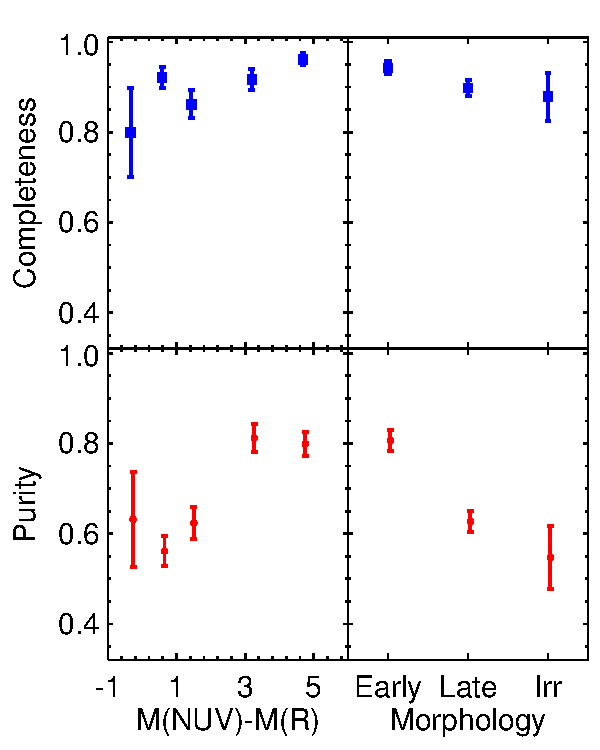
\includegraphics[scale=1]{catalog/f6.pdf}
\caption{Completeness (top row) and purity (bottom row) of the galaxy
  membership selection as measured by the
  spectroscopic subsample for galaxies with $P_{\rm mem}>0.5$. Error bars are
  the standard deviation from 1000 bootstrap samples of the
  spectroscopic catalog. Morphological classes are defined from ZEST
  \citep{Scarlata2007}; the early type category includes ellipticals
  (type=1) and bulge-dominated disks (type=2.0), the late type
  category includes the remaining type=2 sources, and irregulars
  have type=3.} 
\label{cat_fig:memstat_color}
\end{center}
\end{figure}
% **** FIG 6 *****

\subsection{Mock Catalogs}
\label{cat_s:mocks}

We use numerical simulations to construct a series of mock catalogs for a
COSMOS-like survey to test the reliability of our member
selection. Mocks are created from a single simulation (named 
``Consuelo''), part of the Las Damas suite (McBride et al., in prep.)\footnote{Details regarding this simulation can be found at {\url{http://lss.phy.vanderbilt.edu/lasdamas/simulations.html}}}. Consuelo
is a box of $420~h^{-1}~{\rm Mpc}$ on a side with 
$1400^3$ particles of mass $1.87 \times 10^9~h^{-1}~{\rm M}_{\odot}$
and a softening length of $8~h^{-1}~{\rm kpc}$.\footnote{We use
  $H_0=100~h~\rm{km~s^{-1}~Mpc^{-1}}$ in this paragraph only.} 
This simulation can robustly resolve halos with masses above
$\sim10^{11} h^{-1}~{\rm M_{\odot}}$ which corresponds to central
galaxy stellar masses of $\sim10^{8.5}~h^{-1}~{\rm M_{\odot}}$, well-matched
to our completeness limit of F814W=24.2 at $z=0.2$ (see
Figure~\ref{cat_fig:mass_limits}).

We extract ten light cones from the Consuelo simulation that have the
same area as COSMOS and individually non-overlapping volumes. Halos
within the simulation are identified with a friends-of-friends (FOF) halo
finder \citep{Davis1985} with a linking length of $b=0.2$. For typical
halos in the mass range we consider, FOF masses and
spherical overdensity masses (defined within a radius where the mean
density is 200 times the background) typically agree within $\sim10-20\%$
\citep{Tinker2008}; we thus only convert from background to critical
overdensity to obtain \mvir{}.
Halos are populated with galaxies using the HOD model of
\citet{Leauthaud2011a, Leauthaud2011b} 
that simultaneously fits the stellar mass functions, galaxy clustering,
and galaxy-galaxy lensing signals of COSMOS. We adopt the $z \sim 0.6$
HOD model of \citet{Leauthaud2011b} with the following parameters from
Table 5 of that paper:
$\log(M_{1})=12.725$, $\log(M_{*,0})=11.038$, $\beta=0.466$,
$\delta=0.61$, $\gamma=1.95$, $\sigma_{\log \rm  M_{*}}=0.249$,
$B_{\rm cut}=1.65$, $B_{\rm sat}=9.04$, $\beta_{\rm cut}=0.59$, 
$\beta_{\rm sat}=0.740$, $\alpha_{\rm sat}=1$. Details regarding the
parameters in this HOD model can be found in
\citet{Leauthaud2011a}. As shown in \citet{Leauthaud2011b}, there is a
small amount of redshift evolution in this parameter set from $z \sim
0.2$ to $z \sim 1$. However, the redshift evolution should not have a
large impact on our assessment of the completeness and purity of the
group membership selection and so we neglect the redshift evolution of
the HOD in this work.

Galaxies are assigned cosmological redshifts as well as mock
spectroscopic redshifts which include the effect of peculiar
velocities from the velocity dispersion within halos. Photometric
redshifts are drawn from a Gaussian distribution centered around the
spectroscopic redshift with width equal to the photo-$z$ uncertainty for
that magnitude. A Gaussian \pz\ is then centered at \zp\ with the same
width, and sampled at the same redshift interval as the PDF for real
galaxies. We do not include catastrophic photo-$z$ errors which are
shown in Table~\ref{cat_t:photoz_tests} to be a small fraction of the sample. 

The HOD model of \citet{Leauthaud2011a} assigns stellar
masses to mock galaxies but does not assign magnitudes or colors. In
order to apply a similar magnitude cut to the mock galaxies as used in
the selection algorithm, we assign F814W magnitudes to mock
galaxies. For each mock galaxy, we construct a galaxy sample from the
COSMOS data that is matched in redshift and stellar mass in bins of
$\Delta z=0.02$ and $\Delta\log(M_{\star}/M_{\odot})=0.2$. An F814W magnitude
is assigned to each mock galaxy by randomly drawing a magnitude from
the matched sample. We do not assign colors or morphologies to mock
galaxies since the dependence of these properties on redshift and
environment are not well-constrained. We will rely on our
spectroscopic sample in order to determine the completeness and purity
of the group membership selection as a function of color and
morphology instead of using mock catalogs.

Mock halos are given the redshift of the central galaxy and X-ray
luminosities according to the mean $L_{\rm X}-\mvir$ relation of
\citet{Leauthaud2010}. To mimic the position uncertainties of the
X-ray detections, \textsc{xflag} quality flags 1 or 2 are assigned randomly
in proportion to their appearance in the COSMOS group catalog. The nominal
group center is offset from the central galaxy with a Gaussian scatter of $32
\arcsec$ for \textsc{xflag}~=~2 halos which is reduced by the measured flux
significance for \textsc{xflag}~=~1 halos, and we assume a typical
$5\sigma$ flux measurement. The impact of centroiding errors is investigated in
\S~\ref{cat_s:surveys}.

Next we run the membership algorithm described in
\S~\ref{cat_s:membership} on the mock galaxy and halo
catalogs, associating galaxies with halos. We can perform the same
purity and completeness tests as with the spectroscopic sample above,
but this time we know the halo membership \textit{a priori}. The
results from these mock catalog tests are presented alongside those
for the spectroscopic subsample as colored bands in Figures~\ref{cat_fig:memstat_threshold}
and~\ref{cat_fig:memstat_all}.

\subsection{Sources of Error}
\label{cat_s:error}

Results from the tests on spectroscopic data and mock catalogs above
can differ because the spectroscopic sample is weighted toward bright
objects and because our knowledge of true membership in the
spectroscopic data is limited by redshift-space distortions, while
membership in the mock catalogs is known by design. 
The general agreement seen in Figures~\ref{cat_fig:memstat_threshold} and
\ref{cat_fig:memstat_all} between these tests of membership quality is
encouraging, and it suggests that the biases are modest and that the mock
catalogs accurately represent the properties of real galaxies that we
wish to study. The normalization of the purity and completeness curves for the
spectroscopic test has a degree of freedom in the velocity
width used to determine whether a spectroscopic redshift is consistent
with a group redshift. We used the criterion $c|\zs-\zG| < 2\sigma_{\rm
  v}(M,z)(1+\zG)$ for spectroscopic membership; a broader velocity
range for the spectroscopic test would result in a higher measured
level of purity and lower completeness in the photo-$z$ selection, and
the converse holds for a smaller velocity range, shifting the curves
up or down. Though the \textit{absolute} measure of purity and
completeness in the spectroscopic tests holds some degree of
arbitrariness, the \textit{relative} trends shown in
Figure~\ref{cat_fig:memstat_all} are in general agreement with the mocks,
with some offsets likely due to sampling bias and redshift-space
distortions. We study the effects of redshift-space distortions on
member selection in the limit of a completely spectroscopic survey in
\S~\ref{cat_s:surveys}.

Information from the spectroscopic tests has the advantage that it
can probe member selection effects due to properties that cannot easily be
modeled (e.g., galaxy color and morphology), and these tests directly
measure the effects of 
photo-$z$ errors on our selection of galaxies in the same set of
groups. We see in Figure~\ref{cat_fig:memstat_color} that the trends of
selection quality with color and morphology parallel the trends with
magnitude and stellar mass from Figure~\ref{cat_fig:memstat_all}. 
We have shown in \S~\ref{cat_s:photoz_tests} that photo-$z$ quality is
not strongly affected by color or morphology, and no other inputs
to our selection algorithm explicitly depend on these properties. We infer
that the lower completeness and purity seen for faint, low mass, blue, and
late type galaxies is driven by two effects; fainter galaxies have
larger photo-$z$ uncertainties, and galaxies in this population tend to live
outside of dense groups so that they are more likely to be
contaminants when selected.

Because only a fraction of objects have spectroscopic
redshifts, the uncertainties can be large. Tests with mock catalogs
alleviate this issue and provide an
estimate of the sample variance in our selection due to the finite
size of the COSMOS region. An additional advantage of the mocks is
that the central galaxy of  each halo is known, so we can test the
success rate for identifying these objects. We find that $77\%$ of
central galaxies are correctly identified as the MMGG$_{\rm scale}$
galaxies in the corresponding halos, $12\%$ are misidentified as
satellites because the central galaxy is not the most massive member
near the centroid, $5\%$ are misidentified as satellites because the
assigned centroid error puts the galaxy outside of the search region,
and only $5\%$ are assigned to neighboring groups or the field due to
photo-$z$ errors. While the HOD used to create the mocks allows for
satellite galaxies to be more massive than centrals due to scatter in
the relation between stellar mass and halo mass, the fraction of
groups where this occurs is sensitive to the parametrization of the
HOD model and is not well-constrained. The problem of identifying
group centers will be discussed in more detail in Paper II.

For the full sample of mock galaxies with $P_{\rm mem}>0.5$, we find a
mean purity of $67\%$ and completeness of $92\%$. Looking at
Figure~\ref{cat_fig:memstat_all}, it is clear that the dominant source of
impurity comes from galaxies in projection near the outskirts of
groups. We can attribute this contamination to the fact that the
density of true members falls steeply as a function of distance from
group centers while our membership algorithm selects galaxies
uniformly out to \rvir. Faint galaxies are another source of impurity since their
photo-$z$ errors are larger than average. Galaxies with lower masses and
bluer colors are more common in the field than in dense environments
(see \S~\ref{cat_s:discussion}), so a higher contamination fraction from
these populations is to be expected. There is also a slight dependence on halo 
mass, since the density contrast between the field and groups is
smaller for low mass halos, lowering the assigned membership
probabilities of candidate members and reducing the completeness of
the selection. These factors motivate the use of matched filters in
finding groups and clusters when the properties of their galaxy
populations are well-characterized; we have not employed such filters
to avoid biasing our sample and because galaxy properties in this
range of halo masses and redshifts are not thoroughly constrained.

The covariance between these galaxy properties makes it challenging to
isolate their influence on the contamination fraction. For example,
the correlation between the stellar mass and brightness of a
galaxy means that the corresponding panels of
Figure~\ref{cat_fig:memstat_all} are related and not independent probes of
contamination sources. The simplest
way to increase the purity of the group sample is to consider only
galaxies at smaller distances from the group center than the cut of
\rvir\ used here. Restricting the mock sample to $R<0.5\rvir$ results
in a mean purity and completeness of $84\%$ and $92\%$, respectively.

An alternative way to address the contamination and incompleteness of
the selection would be to apply correction factors to the member
selection as a function of these properties, as in
Equation~\ref{cat_eq:correction}. This would amount to introducing strong 
priors to the membership algorithm based on our HOD model, limiting
the independence of the sample. In testing this approach however, we
have noticed that the correction factor as a function of group-centric
radius is not significantly tied to other properties such as
magnitude, stellar mass, or color, indicating that the contamination
is due more to geometry than distinct populations of galaxies. This
suggests that we can reliably study the relative radial trends of
these properties, though the absolute radial trends are subject to
uncertainties in the correction factor.

We can compare the member selection used here with that of
\citet{Giodini2009}, who used a statistical background subtraction on
the same body of data to determine galaxy membership and estimate the total
stellar mass in groups. Because the statistical background approach
does not individually assign galaxies to groups, we cannot
directly compute the purity and completeness of the selection, but we
can compare the total stellar mass estimates from the two selection
methods to the mock values. \citet{Giodini2009} selected candidate members
within a projected radius $R_{500\rm{c}}$ of X-ray centroids and $0.02\times(1+z)$ of the
group redshift, and estimated a mean foreground/background
contribution in 20 non-overlapping field regions of the same size and
redshift. 

We run both member selection methods on the mocks, applying
to each method the same corrections described by \citet{Giodini2009}
to deproject the cylindrical search volume into a sphere of radius
$R_{500\rm{c}}$ and to account for stellar mass contributions below
our sensitivity limit, adapted to the stellar mass function and limits
of our mocks. The mean stellar mass content in groups recovered using
their method is $3\%$ lower ($3\%$ higher) than the input mock value
in the redshift range $0.2<z<0.5$ $(0.5<z<1.0)$. With the same
corrections, our selection method estimates the mean stellar mass to be $3\%$
higher ($9\%$ higher) than the mock values over the same redshift
intervals. The typical scatter of $35\%$ between the recovered values and the
input values for a given group is much larger than the offsets for
both methods, but with these tests on mock catalogs we could remove
the small biases in future measurements. The mean stellar masses
inferred by the two methods happen to be quite similar because they
are typically dominated by massive galaxies for which membership
assignment is relatively straightforward. However, we note
that the full membership selected can be quite different because our approach
optimizes group centers using the weak lensing signal and handles
magnitude-dependent photometric redshift uncertainties, whereas
\citet{Giodini2009} use the X-ray centers and a fixed redshift window. 

We can also test different methods of estimating the field density to
see how it influences our member selection.
Our selection algorithm estimates $\hat{N}_{F}$ from the mean density
across the whole field, but smaller regions could instead be used to
estimate the local density around individual groups. While the local
density estimate has the advantage that it traces correlated structure
around groups, it does suffer from greater shot noise than the density
estimated over a larger volume. We have tested our approach
by using annuli centered on each group with inner and outer radii of
$2\rvir$ and $5\rvir$, while keeping the rest of the selection
algorithm the same. With this approach, the typical field density is
higher due to clustering around groups and the resulting membership probability
is slightly lower (increasing the field density by a factor of 2 typically
lowers the membership probability by only $\sim20\%$), but the purity and
completeness of the sample are essentially unchanged, and the fraction
of members crossing a threshold of $P_{\rm mem}>0.5$ between samples
is less than $10\%$. We obtain
similar results when substituting the background estimation method
used by \citet{Giodini2009} for our field density prior, so the
selection algorithm is not strongly sensitive to the approach used for
background estimation.

\subsection{Applicability to Other Surveys}
\label{cat_s:surveys}

In view of other surveys which will search for groups and clusters in
multi-wavelength data, and to better characterize the advantages or
shortcomings of the COSMOS data used in this analysis, we test our
selection algorithm on mock catalogs with different levels of
uncertainty in redshift and centroid measurements. We consider five
hypothetical data sets: a full spectroscopic survey where all galaxies
have the typical redshift uncertainty in
zCOSMOS\footnote{\url{http://archive.eso.org/archive/adp/zCOSMOS/VIMOS\_spectroscopy\_v1.0/index.html}}
of $\sigma_z=3.7\times10^{-4}$, a low-resolution spectroscopic survey
like PRIMUS \citep{Coil2010} with redshift uncertainties of
$\sigma_z=0.005$, a photometric survey with fewer bands and larger
photo-$z$ errors like SDSS \citep{Csabai2003} or DES \citep{Banerji2008}
with $\sigma_z=0.05$, a deeper X-ray survey with more precise
centroids of  $3\arcsec$, and a lower resolution X-ray or SZ survey with centroid
uncertainties of $1\arcmin$. In the first three mock surveys we vary
only the redshift uncertainty and apply the same centering uncertainty
as the fiducial COSMOS mocks described in \S~\ref{cat_s:mocks} assuming
similar X-ray detections. In the
final two mock surveys we use the magnitude-dependent redshift
uncertainties of the COSMOS mocks and assign centroiding
uncertainties, $\sigma_{\rm X}$, in each dimension on the sky. We
offset the nominal centroid from the central galaxy in each dimension
by a random value drawn from a Gaussian of width $\sigma_{\rm X}$. In all
cases we keep the same group and galaxy detection limits as in the
COSMOS data.

Figures~\ref{cat_fig:memstat_surveys_zerr} and
\ref{cat_fig:memstat_surveys_centroid} show the purity and completeness 
obtained when applying our member selection algorithm to these mock
surveys, in a manner similar to Figure~\ref{cat_fig:memstat_all}. We
reiterate that these statistics describe the accuracy of 
the assignment of galaxies to groups, and not the detection of groups
themselves. The figure illustrates that purity and completeness
improve as redshift and centroid uncertainties decline. A number of
other points can be made about these results:

\begin{itemize}
\item{Deeper and more complete spectroscopic coverage would improve our member
    selection, increasing the purity of the sample from $\sim70\%$
    with photo-$z$s to
    $\sim85\%$. Improvements for completeness would mainly be gained
    from faint galaxies near our magnitude limit.}
\item{Among spectroscopic redshifts, high precision is not
    critical. The completeness of the $\sigma_z=3.7\times10^{-4}$ and
    $0.005$ samples are nearly identical, and the higher precision
    spectra provide only a modest improvement in sample purity over
    the low-resolution spectra, from
    $\sim80\%$ to $\sim85\%$. Once the redshift measurement
    uncertainty becomes comparable to the magnitude of intrinsic
    redshift distortions due to peculiar velocities in groups,
    additional spectral resolution does not greatly improve our ability to
    identify members. PRIMUS data in the COSMOS field will improve
    upon the existing sampling of zCOSMOS, but we note that the completeness
    limit for that survey is $i=22.5$ with sparse sampling to
    $i=23.5$, still shallower than our photo-$z$ depth of F814W=24.2.}
\item{The precise photometric redshifts available in the COSMOS field
    are critical for identifying members using our approach. Redshifts
    that are less accurate or precise show significantly reduced purity
    and completeness.}
\item{The precision of X-ray centroids for COSMOS groups is quite
    sufficient for member selection. Improving the positional
    uncertainty by roughly a factor of eight from the mean COSMOS
    value results in only a few percent improvement in completeness
    and a negligible gain in purity. Conversely, less precise centers
    (such as those available from SZ measurements) produce a sample
    with lower purity in the central region ($\sim85\%$ instead of
    $\sim95\%$) and significantly lower completeness ($\sim75\%$
    instead of $\sim90\%$). Though the existing COSMOS centroids are
    adequate for assigning member galaxies to groups, we note that
    several aspects of groups could still be studied with deeper X-ray
    or SZ data including physical offsets between central galaxies and
    hot gas, and the relationships between temperature or entropy with
    other group properties.}
\item{Note that we do not optimize our selection algorithm for these
    hypothetical data sets. Combining catalogs built from different
    observables \citep[e.g.,][]{Cohn2009}, and other techniques such
    as iterative centering or matched filters could improve results.}
\end{itemize}

We can compare the results of our mock spectroscopic selection to
other methods in the literature. We must note that our definitions of purity and
completeness refer to the success rates for assigning members to known
groups, while previous spectroscopic group-finding efforts have typically
quantified the purity and completeness of the identified group catalog in
addition to the galaxy membership assignment. In our mock tests, we
have implicitly assumed that the identification of groups is pure and
complete. It is also difficult to make direct comparisons across surveys
because of differences in data sets, limiting depths, and mock
catalogs. However, looking briefly at the quoted purity and
completeness of spectroscopic group catalogs, we can assess our
algorithm and see the advantage to assigning group membership when the
existence of a group is already know (e.g., from an X-ray detection).

Using a tesselation method to find galaxy groups in DEEP2 with a
limiting galaxy magnitude of R$_{\rm AB}=24.1$,
\citet{Gerke2005} attained a mean interloper fraction (analogous to
our impurity, $1-\mathsf{p}$) of $f_I=0.458\pm0.004$ and a mean galaxy
success rate (analogous to our completeness) of $S_{\rm
  gal}=0.786\pm0.006$ in their mock tests. They reported a one-way group identification
purity of $P_1=0.545\pm0.005$ and completeness of
$C_1=0.782\pm0.006$. \citet{Knobel2009} found that a
friends-of-friends approach performed better than the tesselation
method for identifying groups in zCOSMOS to a limiting magnitude of
I$_{\rm AB}=22.5$, and reported values of
$f_I=0.29$, $S_{\rm gal}=0.84$, $P_1=0.66$, and $C_1=0.81$ from their mocks. These
values are for groups with $N_{\rm mem}\ge2$, and while
\citet{Gerke2005} showed values for group purity and completeness that
were roughly constant with group velocity dispersion,
\citet{Knobel2009} showed that each of these statistics improved when
restricting the sample to higher richness groups, flattening out for
groups with $N_{\rm mem}\gtrsim5$. Disentangling the effects of group
identification from galaxy membership assignment is difficult, but
since the reported $S_{\rm gal}/C_1$ and $(1-f_I)/P_1$ are both
approximately unity, it appears that the main challenge in assigning
galaxy membership with these algorithms is in identifying real
groups. This fact illustrates the advantage of combining group-finding
methods to ensure a reliable sample of groups before assigning members.


% **** FIG 7 *****
\begin{figure}
\plotone{catalog/f7.pdf}
\caption{Completeness (top row) and purity (bottom row) of the galaxy
  membership selection for hypothetical surveys with different
  redshift uncertainties according to the legend. Each curve
  represents the mean of ten mock lightcones. The fiducial survey is the same as
  that plotted in Figure~\ref{cat_fig:memstat_all} for COSMOS. Note that
  the completeness curves for $\sigma_z=0.0004$ and $0.005$ lie atop
  one another.}
\label{cat_fig:memstat_surveys_zerr}
\end{figure}
% **** FIG 7 *****

% **** FIG 8 *****
\begin{figure}
\plotone{catalog/f8.pdf}
\caption{Completeness (top row) and purity (bottom row) of the galaxy
  membership selection for hypothetical surveys with different
  centroid uncertainties according to the legend. As in
  Figure~\ref{cat_fig:memstat_surveys_zerr}, each curve represents the
  mean of ten mock lightcones, and the fiducial survey is the same as 
  that plotted in Figure~\ref{cat_fig:memstat_all} for COSMOS.}
\label{cat_fig:memstat_surveys_centroid}
\end{figure}
% **** FIG 8 *****


%--------------------------------------------------------
% --------------   SECT 6
%--------------------------------------------------------

\section{Member Catalog}
\label{cat_s:catalog}

In the spirit of public releases of COSMOS data, we make our
membership assignments available as machine-readable files through the
NASA/IPAC Infrared Science Archive
(IRSA)\footnote{\url{http://irsa.ipac.caltech.edu/Missions/cosmos.html}}.
These data include galaxy positions, redshifts, stellar masses,
colors, and membership probabilities, along with group
identifications. For each group we provide the X-ray position, flux,  
and luminosity, along with the redshift, halo mass, quality flags, and
the position and stellar mass of the central galaxy MMGG$_{\rm scale}$.
For reference, the basic parameters describing the catalog are compiled in
Table~\ref{cat_t:catalog_properties}. For analyses requiring a clean
selection of galaxy groups, we restrict the sample to groups with
\textsc{xflag}~$=1$ or 2 and the \textsc{mask}, \textsc{poor}, and
\textsc{merger} flags blank to ensure that groups
and members have been reliably identified; in the group catalog we
define a new property, \textsc{flag\_include}, to encode this combination of
selection cuts. When a pure and complete
sample of members is needed, we select galaxies with $P_{\rm mem}>0.5$
in the inner regions of groups, $R<0.5\rvir$, with stellar masses
above our sample limit shown in Figure~\ref{cat_fig:mass_limits}.

\begin{deluxetable}{lc}
\tabletypesize{\scriptsize}
\tablewidth{0pt}
\tablecaption{Basic catalog properties\label{cat_t:catalog_properties}}
\tablehead{\colhead{Property} & \colhead{Value}}
\startdata
Field coordinates (J2000) & RA=(149\fdg4, 150\fdg8), Dec=(1\fdg57, 2\fdg90) \\
Group redshift & $0 < \zG\ < 1$ \\
Galaxy magnitude & F814W~$<24.2$ \\
Halo mass & $12.8 < \log(\mvir/M_{\odot}) < 14.2$ \\
X-ray luminosity & $41.3 < \log(L_{\rm X}/\ergsec) < 44.1$ \\
N$_{\rm groups}$ & $211$ \\ 
N$_{\rm groups}$ (\textsc{xflag}~$=1,2$) & $165$ \\  
N$_{\rm groups}$ (clean groups\tablenotemark{a}) & $129$ \\  
N$_{\rm mem} (P_{\rm mem}>0.5)$ & $4639$ \\
N$_{\rm mem} (P_{\rm mem}>0.5$, clean groups) & $3415$ \\ 
N$_{\rm mem} (P_{\rm mem}>0.5, R<0.5\rvir, \log(M_{\star}/M_{\odot})>10.3)$ & $867$ \\
N$_{\rm mem} (P_{\rm mem}>0.5, R<0.5\rvir, \log(M_{\star}/M_{\odot})>10.3$, clean groups) & $656$
\enddata

\tablenotetext{a}{\textsc{xflag}~$=1,2$, \textsc{mask}=\textsc{poor}=\textsc{merger}=0}
\end{deluxetable}

In addition to the catalog described above using photometric
redshifts, we have also produced a catalog replacing photo-$z$s with
spectroscopic redshifts when available. We use the same selection
algorithm and replace \pz\ from the photo-$z$ with a Gaussian of width
equal to the typical uncertainty in zCOSMOS, $\sigma_z=3.7\times10^{-4}$, and
sample each distribution at intervals of $10^{-5}$ in redshift. This
catalog has better purity and completeness than the photo-$z$ catalog
because of the improved redshift accuracy, but the selection is less
homogeneous because spectroscopic sampling is not representative or
complete.


%--------------------------------------------------------
% --------------   SECT 7
%--------------------------------------------------------

\section{Analysis and Discussion}
\label{cat_s:discussion}

With the catalog of group members identified and the purity and
completeness of the sample characterized, we provide a first look at
the properties of galaxies in these groups. Here we present
an analysis of the colors of group members
relative to the field. Future papers will study member properties in
more detail, including galaxy morphologies, star formation rates, and
AGN activity with respect to group properties like redshift, halo
mass, and group-centric distance.

Figure~\ref{cat_fig:group_cm} shows the unextincted rest-frame NUV-R
colors from \citet{Ilbert2010} for group members. We use the clean
sample of groups, selecting members with $P_{\rm mem}>0.5$ within
\rvir\ of the group center. The apparent banding in colors is due to
the finite number of templates used. We call
galaxies identified as the MMGG$_{\rm scale}$ ``centrals'' with the
other members as ``satellites.'' We see a
bimodal distribution in color space for both central and satellite
galaxies, though redder colors are more common than blue for both
types of members. In the margin plots, we show the distributions of
colors and stellar masses for centrals and satellites, as well as
field galaxies not assigned to any X-ray detected group ($P_{\rm
  mem}=0$). The field sample has been selected to match the redshift
distribution of group members in bins of $dz=0.1$. Although the color
distribution of field galaxies is also bimodal, it is clear that bluer
galaxies are more common in the field than in groups, a well-known
result in clusters and dense environments over a range of mass scales
and redshifts \citep[e.g.,][]{Gerke2007}.

We also see that there exist a number of blue centrals, which are of
interest because they suggest that star formation can persist or be
reactivated in the centers of dense groups, or that AGN exist there. The set of red
points in Figure~\ref{cat_fig:group_cm} omits ambiguous cases where there
is a more massive galaxy in the outskirts of a group or where the
MMGG$_{\rm scale}$ differs between the photo-$z$-only catalog and
the one supplemented with available spectroscopic redshifts; $79\%$ of
groups satisfying the quality cuts of \S~\ref{cat_s:catalog} have an
unambiguous central according to these criteria. While the majority of
this sample of centrals are red (77 out of 102), there are 5 centrals
with blue colors indicative of active star formation or AGN, and 20 centrals
with colors indicating intermediate activity. This population warrants
further study to verify that they are accurate centers and to
determine what environmental factors could contribute to the star
formation or AGN activity.

% **** FIG 9 *****
\begin{figure}
\plotone{catalog/f9.pdf}
\caption{Stellar masses and unextincted rest-frame template colors for
  central galaxies (red diamonds) and satellites (gray dots). We plot
  only the unambigous centrals, \ie those 
  designated as the MMGG$_{\rm scale}$ in groups which do not have a more
  massive galaxy in the outskirts or a discrepancy between
  identification with spectroscopic and photometric redshifts. Horizontal 
  dashed black lines show the galaxy spectral classes of
  \citet{Ilbert2010}. Margin plots show the distribution of colors and
stellar masses for centrals (red solid), satellites (gray dashed), and
a redshift-matched sample of field galaxies (blue dotted), rescaled
for comparison. Axis labels should be multiplied by 15 (centrals), 150
(satellites), and 500 (red-shift matched field sample)
to obtain the normalized distributions. The lower end of the stellar
mass range plotted corresponds to our completeness limit at $z=1$.}
\label{cat_fig:group_cm}
\end{figure}
% **** FIG 9 *****
 
\subsection{Environmental Dependence from $z=0.2$ to $1$}

The higher fraction of blue galaxies in the field compared to groups
shown in Figure~\ref{cat_fig:group_cm}
indicates that star formation is less common in dense
environments. As discussed in the introduction, much work has been
carried out to determine whether this well-known effect is due to a physical
process acting on galaxies in dense enviroments to suppress their star
formation rates, or due to the intrinsic properties of galaxies that
exist in these regions. 

To distinguish between the possibilities of environmental influence
and innate differences, we compare galaxy colors in group and field
environments within fixed stellar mass bins. We measure the fraction
of galaxies of the quiescent type defined by \citet{Ilbert2010}, \ie\
those with $M(NUV)-M(R)>3.5$. These are unextincted rest-frame colors
from the spectral template that best fits each galaxy's SED, allowing
us to study intrinsic colors that are related to specific star
formation rates without the obscuring effects of dust. The correction
is important because galaxies in low density environments have a higher dust
content, even among massive galaxies \citep{Kauffmann2004}. 

The fraction of red galaxies in fixed stellar mass bins is plotted
for three redshift ranges in Figure~\ref{cat_fig:quenchz}. For group
members, we consider only galaxies with membership probability $P_{\rm
mem}>0.5$ within a projected distance of $0.5\rvir$ of the center of
groups in the mass completeness-limited bins of
Figure~\ref{cat_fig:mass_limits}. The radial cut on the group sample is to avoid contamination
in the outskirts discussed in \S~\ref{cat_s:error}. The plot includes both centrals and
satellites; excluding centrals leaves the results essentially
unchanged because the sample is dominated by satellites even in the
highest stellar mass bin plotted. The fraction of red galaxies in
this population is plotted against the mean stellar mass for each
bin. We also plot the red fraction in individual groups for galaxies
in the same stellar mass bins to show the
variation between groups. At all redshifts, higher mass galaxies tend
to have higher red fractions than lower mass galaxies. In addition to
this stellar mass dependence, we see a clear separation
between the group and field populations at all redshifts for the
stellar masses probed. The field sample plotted matches the
the redshift bins used for group members; matching the redshift
distribution on finer scales results in quenched fractions
that are at most a few percent different from those plotted.

We also see evidence for an increase in the red fraction with
decreasing redshift among low mass group galaxies. Redshift 
trends are somewhat difficult to interpret because the
range of group masses used is different in each redshift bin (see
Figure~\ref{cat_fig:mass_limits}) and the color cut does not account for
evolution, so we leave a detailed analysis for
future work. Because our galaxy sample is magnitude-limited,
the low mass bins at high redshift are incomplete and plotted as open
symbols. We make no corrections for incompleteness here, which likely
leaves the sample in these bins biased toward the detection of blue
galaxies that tend to have lower mass-to-light ratios than red galaxies,
so we consider the red fractions in incomplete bins to be lower limits.

% **** FIG 10 *****
\begin{figure}
\plotone{catalog/f10.pdf}
\caption{Fraction of quenched galaxies as a function of stellar mass
  in different redshift bins (separate panels). Triangles show the
  quenched fraction of members with $P_{\rm mem}>0.5$ and
  projected group-centric distance within $0.5$\rvir\ of groups in the
  mass bins from Figure~\ref{cat_fig:mass_limits}. Squares show the
  quenched fraction of field galaxies with $P_{\rm mem}=0$. Open
  symbols show bins with stellar mass incompleteness; the arrows above
  these symbols indicate that they are likely to be biased lower than
  the true values. Vertical error bars show the standard deviation of 1000
  bootstrap samples and horizontal bars represent the stellar mass bin widths. Gray circles
  show the quenched fraction in a given stellar mass bin for
  individual groups, with size proportional to the number of members
  in the bin. Note that the range of halo masses for group members
  varies between redshift bins.}
\label{cat_fig:quenchz}
\end{figure}
% **** FIG 10 *****
 
We detect a clear dependence of galaxy color on environment, even at fixed
stellar mass and high redshift. Figure~\ref{cat_fig:quenchz} uses the
member catalog determined with photometric redshifts only, but
including the available spectroscopic redshifts does not affect the
results. Our results are similarly insensitive to the choice of a
probability threshold for membership; changing the cut on $P_{\rm
  mem}>0.5$ to 0.3 or 0.7 or weighting objects by $P_{\rm mem}$ instead
of choosing a threshold moves the red fractions by no more than a
few percent in any bin. Using the color
cuts described in \citet{Bundy2010} to separate passive galaxies in
COSMOS from dusty star-forming galaxies also gives qualitatively similar
results. Though the absolute fraction of red galaxies measured depends
on the specific cuts used, the relative trends with stellar mass and
environment are similar; galaxy groups have a larger proportion of red
galaxies than the field, and groups dominated by blue galaxies are
rare, though some appear to exist. 

We note that while our results confirm a significant relationship
between color and environment out to the redshift limit of our sample,
the cause of this relationship remains unknown. More detailed analysis
distinguishing between physical processes happening before and after
galaxies join groups is necessary to determine the role that groups
play in this process.

We now compare Figure~\ref{cat_fig:quenchz} to results from the literature.
Our findings are consistent with results at low-redshift that show a
decrease in star formation at high stellar masses, as well as a clear
connection between star-formation and environment even after
accounting for stellar mass differences 
\citep[e.g.,][]{Kauffmann2004, Baldry2006}. At $z\sim0.4$,
\citet{McGee2011} report an environmental trend in the GEEC
survey that is smaller than a comparable low-redshift sample, but
still significant. However, \citet{Poggianti2008} do not detect a significant separation in
the fraction of star-forming galaxies in cluster and field environments at
$z=0.4-0.8$ after matching stellar mass distributions. 

At the highest redshift range covered by our group sample, our
findings are consistent with those of \citet{Cooper2010} and 
\citet{Peng2010} who detect a significant color-density relation in
a similar stellar mass range covered by DEEP2 and
zCOSMOS, respectively. These results appear to be at odds 
with some claims from VVDS and zCOSMOS analyses that such a relation
could be attributed solely to the existence of more massive galaxies
in dense environments
\citep[e.g.,][]{Scodeggio2009,Cucciati2010,Iovino2010}. Each of these
studies consider the environmental effect on color at fixed stellar
mass, as we have done here. \citet{Cooper2010}
emphasize that systematics in the selection of dense environments tend
to wash out the measured signal of environmental dependence, so that if such
correlations are seen they are likely to be real.
They also suggest that the non-detection of environmental trends in other
surveys is likely due to lower spectroscopic sampling rates and
reliance on less confident redshifts which comprise a significant
fraction of the sample at high redshift. The photometric
redshifts used in the present work are certainly less precise than
spectroscopic redshifts, but have a much higher sampling density. 

An important distinction with this study is that we are using a unique sample of groups;
X-ray detections ensure a robust sample of structures that are
virialized, a trait which may not be true of optically-selected
groups. The X-ray groups are also more massive than the typical
spectroscopically-selected groups, and may have formed earlier giving
them a longer time to suppress star formation in member
galaxies. Other studies of this sample of X-ray groups also detect a
significant environmental effect on galaxy colors (Giodini et al., in
prep.; Tanaka et al., in prep.). \citet{Finoguenov2010} have shown
that the number density of this X-ray group sample is in reasonable
agreement with that expected for halos of corresponding masses within
our cosmological model. The sample is therefore unlikely to be an extreme
population of groups, though we cannot rule out subtle differences
between X-ray-selected groups and the full population of groups in
this mass range.

Because of differences in analysis methods, it is difficult to
determine whether the qualitatively distinct findings in these
environmental studies are also quantitatively inconsistent, or whether
different results are simply due to measuring different quantities.
We now consider aspects of the analysis methods and
definitions of environments that may contribute
to the differing results, focusing our attention to field studies at $z\sim
1$ where the results appear most discrepant. For instance, we have shown in
Figure~\ref{cat_fig:memstat_surveys_centroid} that centroiding errors can
influence the purity and completeness of a 
group sample, and our lensing tests (see Paper II) ensure a reliable
determination of the center of mass. Additionally, we use only galaxies and groups in
mass-complete bins, avoiding the need for volumetric corrections made
in some of the previous analyses.

Our group-based definition of 
dense environments is most similar to that of \citet{Iovino2010}, who
studied optically selected groups which are less massive on average
than the X-ray groups studied here. We leave a detailed comparison
between optically and X-ray selected groups in COSMOS to a
future paper (Finoguenov et. al, in prep.), but Figure 22 of \citet{Kovac2010a}
shows that these X-ray selected groups tend to be in more dense regions
on average than the optically selected ones. The richest optical
groups (with 4 or more members) show a good correspondence with X-ray
groups in the density field and are more likely to have similar halo
masses. Figure 12 of \citet{Iovino2010} shows that the colors of
stellar mass-selected samples do not significantly depend on group
richness (except perhaps at low stellar mass and redshift), so the
difference in halo masses between X-ray and optical groups is not
obviously the cause of discrepancy between our results and those of
\citet{Iovino2010}. \citet{Knobel2009} tested the purity of the
optical group sample with mock catalogs and found a contamination
fraction of roughly $25\%$, improving to about $15\%$ for richer
groups. These values are similar to our estimate of $16\%$
contamination within $0.5\rvir$ for the sample used in our analysis,
so the correct identification of group members is not a clear cause for
the difference in results either.

\citet{Cucciati2010} quantify environment using the local galaxy
overdensity $\delta=(\rho-\bar{\rho})/\bar{\rho}$, where $\rho$ is the
local density computed from the distance to the fifth nearest neighbor
and $\bar{\rho}$ is the mean density at a given redshift. Their Figure
10 shows a red fraction that is roughly constant across quartiles
of the local overdensity distribution for $z>0.5$ and
$\log(M_{\star}/M_{\odot})>10.85$, with a weak overdensity dependence at lower
redshift. With the same data and density indicator, \citet{Peng2010}
study the density field $\rho$ 
instead of the overdensity field $\delta$ and show a
significant color-density relation at $z\sim0.5$ and state that it continues to at
least $z=1$. They attribute the
difference in results to the fact that a lower fraction of galaxies at
$z\sim1$ live in regions with high $\delta$, and so the highest overdensity
quartile used in the analysis of \citet{Cucciati2010} is presumably too
broad at $z\sim1$ to isolate the small population of galaxies in
regions dense enough to produce strong environmental
effects. \citet{Cooper2010} use a third nearest neighbor density
estimator on DEEP2 data and identify a difference in the
distribution of colors between galaxies in the upper $10\%$ and lower
$50\%$ of the density distribution, so perhaps a cut more stringent
than the upper quartile of the density distribution is needed to detect
environmental effects at $z\sim1$.  Referring again to Figure 22 of
\citet{Kovac2010a} however, we see that X-ray groups live in roughly
the same range of overdensities as the upper
quartile of $\delta$ used in the \citet{Cucciati2010} analysis
($\log(1+\delta)\gtrsim1$). Thus the explanation from \citet{Peng2010}
for the non-detection of environmental trends at $z\sim1$ by
\citet{Cucciati2010} is not obviously applicable since we see a clear
environmental signal in this overdensity range.

The scale on which environment is defined also differs between these
analyses. The fifth nearest neighbor estimator used by
\citet{Cucciati2010} and \citet{Peng2010} and third nearest neighbor
used by \citet{Cooper2010} measure environment on a
scale that varies with density and is typically of order
$1~\rm{Mpc}$. \citet{Scodeggio2009} measures a density field on a
significantly larger scale of $8~\rm{Mpc}$, so correlations on the
smaller scales of group halos may be washed out. The group sample in
Figure~\ref{cat_fig:quenchz} is restricted to $0.5\rvir$ but the
environmental signal is not significantly different when all selected
members out to \rvir\ are included, despite the higher contamination
fraction. In either case, \rvir\ is typically about $500~\rm{kpc}$ for
these groups, so our sample is likely probing the environment on
smaller scales than studies using the galaxy density field.

Differences in the colors used to identify galaxies as red or blue
could also contribute to the contrasting results. The other studies
discussed here typically use rest-frame $U-B$ or $B-I$ colors,
sometimes with a mass or redshift dependent cut to account for varying
populations. We use an extinction-corrected rest-frame $NUV-R$ color
to account for unquenched galaxies that appear red due to dust. To
test the effect of this correction, we have tried redefining the
sample of red galaxies using the cuts $NUV-R>3.5$ or $U-B>1$ without
any extinction correction. The red fraction increases due to the influence of dust
redding, and the separation between group and field values at $z>0.5$
is reduced by up to a factor of $2$, but we still see a clear
difference between the red fraction in group and field environments.

We have not identified an obvious single factor to explain why previous
analyses did not detect an environmental effect on galaxy color, but
suspect the cause to be a combination of factors mentioned above. To
avoid confusion when discussing environmental effects and to properly
detected these trends, it is clearly important to specify what is
meant by ``environment'' and to measure it carefully. 

\subsection{Star Forming Galaxies and the SZ Power Spectrum}

Recent high-resolution, ground-based experiments have probed the power
spectrum of the CMB to unprecedented fine scales (e.g., $\ell \gtrsim 2000$;
\citealt{Lueker2010, Fowler2010, Shirokoff2010, Das2011}), which are
sensitive to a variety of secondary 
anisotropies, such as radio and submillimeter point sources, and the SZ
effect from groups and clusters.  It was found that the power
due to the SZ effect was 50\% or less than predictions of most of the models
\citep{Lueker2010, Dunkley2010}, which could be indicative of our incomplete
understanding of the properties of groups and clusters, especially the low mass
($<10^{14} M_\odot$) systems at $z>0.5$, as they are believed to contribute
half of the SZ power at $\ell\approx 3000$
\citep[e.g.,][]{Komatsu2002, Shaw2010, Trac2011}.  It is possible
that the hot gas pressure profile of distant groups behaves differently from
that of clusters or that cluster profiles deviate from expectations at
large radii, although it was recently shown that local groups obey the
``universal'' pressure profile \citep{Sun2011} and at least one nearby
cluster obeys the profile out to \rvir\ after accounting for gas clumping
\citep{Simionescu2011}.  Another possibility is that star 
formation (SF) activity is elevated in high-$z$ systems, and the contribution
of unresolved SF galaxies in the submillimeter regime could fill in the SZ decrement at $\sim
150$ GHz, thus reducing the SZ power \citep[e.g.,][]{Hall2010}.  Using
the $z=0.5-1.0$ COSMOS groups, we are in a good position to
investigate the contamination due to SF galaxies in groups.

For each group, we cross-matched all candidate member galaxies with the MIPS
$24~\mu$m source catalog \citep{Sanders2007,LeFloch2009}, using a matching radius of $2''$.  For the
matched objects, we assumed a starburst SED (spanning from $3600$\AA\ to $1~\rm{cm}$)
taken from \citet{Lagache2003}, and compared the $24~\mu$m to 148 GHz flux ratio.
More specifically, we approximated the MIPS $24~\mu$m band as a tophat spanning
20.8 to 26.1~$\mu$m, and we used 18 GHz as the bandwidth for the 148 GHz
channel of the Atacama Cosmology Telescope (ACT).  Given the mass of
our groups, we estimated the SZ flux for our 
groups, following \citet{Majumdar2004}. We find that the sum of the fluxes from SF
galaxies at 148 GHz is negligible (typically $\lesssim 0.3\%$) compared to the magnitude of the SZ
effect from these groups. 

We selected the SED from the set of templates of \citet{Lagache2003}
that maximizes the 148 GHz to $24~\mu$m flux ratio to set a
conservative upper limit, but uncertainties in the spectral model
could allow for a larger flux at millimeter wavelengths from these
sources. \citet{Lee2010} compare stacked MIPS measurements at 24, 
70, and 160~$\mu$m to empirical templates from \citet{Chary2001,
  Dale2002, Lagache2003} and theoretical models from
\citet{Siebenmorgen2007}. For the stacked MIPS fluxes of sources at
$z=0.5-1$, the best-fitting template from \citet{Lagache2003} tends to
predict a flux at wavelengths longer than $300~\mu$m that can be an order of
magnitude lower than other models. Even accounting for these uncertainties
in the spectral models, our upper limit to the contamination of
star-forming galaxies to the SZ signal from our sample of groups is no
more than a few percent.

Our group sample is limited to $z<1$.  Several studies have reported
elevated SF activity in centers of clusters at $z\gtrsim 1.4$ \citep[e.g.,
][]{Hilton2010,Tran2010,Tanaka2010}.  It remains to be seen if the SF galaxies could
be abundant enough at higher redshifts to make a significant impact on
the SZ signal in such systems.


%--------------------------------------------------------
% --------------   SECT 8
%--------------------------------------------------------

\section{Summary and Conclusions}
\label{cat_s:conclusion}

We have presented a catalog of member galaxies in X-ray selected
groups in the COSMOS field, carefully taking into account photo-$z$
errors and attempting to avoid biasing the sample with assumptions
about the properties of galaxies which have not previously been
well-constrained in this mass and redshift range. We have thoroughly
characterized the quality of the selection algorithm using tests with
mock catalogs and spectroscopic redshifts. In these tests we
discovered contamination from galaxies in projection in the outskirts
of groups, but selection in the central regions is relatively clean. 
We have also studied the prospects for applying this selection
algorithm to future multi-wavelength data sets, estimating the purity
and completeness of the member selection as a function of redshift and
centering uncertainties.

Analyzing this sample of group members, we have shown that both
stellar mass and environment play a role in determining galaxy colors
at $z\sim 1$. We emphasize that there are many ways to smear out
environmental correlations and that these factors must be properly
controlled in order to detect environmental trends. The X-ray
groups studied here provide a clean sample of dense environments for
which we can determine halo masses and centers.

Following our finding of suppressed star formation in group
environments at all redshifts sampled, we investigated the possibility
that clustered dusty star-forming galaxies could reduce the detected power in the
high-$\ell$ CMB power spectrum by filling in SZ decrements in
groups, and found that the effect must be quite small in this group
sample. In contrast with the results relating to the suppression of
star formation in groups, we have identified several blue
central galaxies, which warrant further study.

In Paper II of this series on our sample of galaxy groups and members, we
will describe weak lensing tests used to optimize the centering by
finding tracers that best locate the center of mass. Further work
will analyze galaxy properties in groups with respect to the distance
from these centers, providing constraints on models describing the
evolution of galaxies in dense environments. With a
carefully selected sample of member galaxies in groups with
well-constrained masses and centers, we can hope to map the course by
which galaxies transform.


\chapter{Galaxies in X-ray Groups. II. A Weak Lensing Study of Halo Centering}

\label{chap:centering}

%-------- ABSTRACT  ---------------------
  
  Locating the centers of dark matter halos is critical for
  understanding the mass profiles of halos as well as the formation and
  evolution of the massive galaxies that they host. The task is observationally
  challenging because we cannot observe halos directly, and tracers
  such as bright galaxies or X-ray emission from hot plasma are
  imperfect. In this paper we quantify the consequences of miscentering on
  the weak lensing signal from a sample of 129 X-ray selected galaxy
  groups in the COSMOS field with redshifts $0<z<1$ and halo masses in
  the range $10^{13}-10^{14}~{\rm M_{\odot}}$. By measuring the
  stacked lensing signal around eight different candidate centers
  (such as the brightest member galaxy, the mean position of all
  member galaxies, or the X-ray centroid), we determine which
  candidates best trace the center of mass in halos. In this sample of
  groups, we find that massive galaxies near the X-ray centroids
  trace the center of mass to $\lesssim 75$~{\rm kpc}, while the X-ray 
  position and centroids based on the mean position of member galaxies
  have larger offsets primarily due to the statistical uncertainties in their
  positions (typically $\sim50-150~{\rm kpc}$). Approximately $30\%$ of
  groups in our sample have ambiguous centers with multiple bright or
  massive galaxies, and some of these groups show disturbed mass
  profiles that are not well fit by standard models, suggesting that
  they are merging systems. We find that halo mass estimates from stacked
  weak lensing can be biased low by $5-30\%$ if inaccurate centers are
  used and the issue of miscentering is not addressed. 

\section{Introduction}

Galaxy groups and clusters are important sites of galaxy evolution and
the abundance of these massive objects provides a sensitive probe of
the amplitude of matter fluctuations and other cosmological
parameters. Analyses of these structures require some knowledge of the
location of the centers of their gravitational potentials. Because the
total mass distribution is dominated by dark matter and is not
directly observable, halo centers are typically assumed to be traced
by a massive galaxy or the density peak of radiating hot
gas. Miscentering is a critical issue when estimating the masses 
of groups and clusters because it adds significant systematic
uncertainties \citep[e.g.,][]{Johnston2007a, Johnston2007b,
  Mandelbaum2010, Rozo2011}, and also degrades constraints on the
concentration of mass profiles \citep{Mandelbaum2008}. Velocity
offsets between observational tracers and halo centers impact studies
of satellite kinematics \citep{Skibba2011, Wojtak2011} and
redshift-space distortions \citep{Hikage2012}. On the other hand, offsets between
observational tracers and the true halo centers can provide information about
the dynamical state of these systems and about the properties of dark
matter \citep{Clowe2006, Massey2011}.

Finding halo centers is challenging for a number of reasons. Galaxy
formation models (as well as halo models for describing the
multiplicity of galaxies within halos) typically place the brightest
or most massive galaxy at the center of each halo. But the brightest
galaxy in a cluster is not always the central galaxy \citep[][and
references therein]{Skibba2011}. Groups and clusters form from mergers
of halos where the most massive halo becomes the host halo with its
central galaxy, and smaller halos become subhalos with satellite
galaxies. Several analyses of data from group
    catalogs and field surveys have found that there is some intrinsic scatter
    in stellar mass and luminosity at fixed halo mass \citep{Yang2009,
      More2009, Leauthaud2012, Reddick2012}, which implies that
    halos can end up with satellites that are intrinsically more
    massive or luminous than the central galaxy. Additionally, there are
uncertainties in measuring any observable quantity such as stellar
mass that can cause a satellite to be misidentified as the most
massive central galaxy, and structure projected along the line of
sight can confuse the identification of member galaxies. Another difficulty
is that merging systems are dynamically unrelaxed, which can produce offsets
between the central galaxy and the halo center or other tracers such
as the X-ray center.  The systematics introduced by picking centers
that do not coincide with the ``true'' center of mass are important
and need to be quantified.

Gravitational lensing is a powerful tool for finding the centers of mass of halos
since it is sensitive to the total mass distribution along a line of
sight. Mass maps can be constructed for individual systems with strong
lensing or for massive clusters with weak lensing
\citep[e.g.,][]{Smith2005b, Oguri2010, Shan2010}. Such studies often 
find reasonable agreement between the positions of bright massive
galaxies, X-ray emission, and lensing mass peaks, with a handful of
interesting examples that illustrate how dark matter peaks can be
offset from hot gas in merging galaxy clusters
\citep[e.g.,][]{Clowe2004, Bradac2008}. 

In this paper, however, we are concerned with a large statistical
sample of groups with lower masses and higher redshifts, a regime of
interest for many current and future weak lensing surveys. The typical
signal-to-noise ratio for the weak lensing signal from individual groups is
low, so we cannot identify their halo centers individually. By stacking
the lensing signal from many groups, we determine the mean mass
profile around a given center. We repeat this process for
different candidate centers and compare the resulting profiles to find
the best tracer of the center of mass.
The center of a smooth halo can be identified as the position where
the lensing signal is maximized on small scales. Other components such
as a massive galaxy or subhalo that is offset from the halo center
could produce an additional peak in the lensing signal, so we must
account for that when modeling the signal.

We analyze a sample of 129 X-ray selected galaxy groups at redshifts
$0<z<1$ from the COSMOS field \citep{Scoville2007a}, described in
\citet{George2011}.  With 
COSMOS data, we have X-ray luminosities and centroids for each group,
with member galaxies identified using photometric redshifts derived
from over thirty ultraviolet, optical, and infrared bands, and a
subsample with spectroscopic redshifts. We use weak lensing
measurements from high resolution \textit{Hubble} imaging to study the
accuracy with which tracers such as bright galaxies and X-ray emission
identify the centers of dark matter halos.

This paper is the second in a series studying the galaxy content of
X-ray groups. \citet[][hereafter Paper~I]{George2011} presented a
catalog of group membership assignments from a Bayesian treatment of
photometric redshifts, along with extensive tests of the selection
algorithm using mock catalogs and subsamples with spectroscopic
redshifts. Initial analyses of group members were used in that paper
to demonstrate an environmental influence on galaxy colors out to
$z=1$. A previous weak lensing study of this group sample was used to
constrain the mean relation between X-ray luminosity and halo mass
\citep{Leauthaud2010}. 

In this paper we study the centers of groups in
detail to optimize observational choices for centering, to study the
impact of miscentering on measurements of halo properties, and to
explore the effects of merging and substructure on lensing
measurements. The outline of the paper is as follows. Section~\ref{cen_s:data} describes the data used in our
analysis, including the X-ray group catalog, assignment of member galaxies,
and lensing shape measurements. We define eight candidate group
centers in Section~\ref{cen_s:centers}, and describe our procedure for
testing different choices of centers in Section~\ref{cen_s:lensing}. Section~\ref{cen_s:results}
presents the results of our analysis, and Sections~\ref{cen_s:discussion}
and~\ref{cen_s:conclusion} provide discussion and conclusions of our work.

We adopt a WMAP5 $\Lambda$CDM cosmology with $\Omega_{\rm m}=0.258$,
$\Omega_\Lambda=0.742$, $H_0=72$ $h_{72}$ km~s$^{-1}$~Mpc$^{-1}$
\citep{Dunkley2009} following the initial lensing analysis of these
groups by \citet{Leauthaud2010}. All distances are expressed in
physical units with $h=0.72$. X-ray luminosities are expressed in the 0.1-2.4 keV
band, rest-frame. All magnitudes are given on the AB system. To
approximate the virial radii of halos, we use $R_{\rm 200c}$ which is
the radius within which the mean mass density equals 200 times the
critical density of the Universe at the halo redshift, $\rho_{\rm
  c}(z)$. The corresponding mass enclosed within this radius is
$M_{\rm 200c}=200\rho_{\rm c}(4\pi/3)R_{\rm 200c}^3$. We also assume
halos follow a Navarro-Frenk-White \citep[NFW, ][]{Navarro1996} density
profile, with a concentration parameter $c_{\rm 200c}$ and a scale radius
$R_{s}=R_{\rm 200c}/c_{\rm 200c}$. We use the term ``group'' to 
denote a set of galaxies occupying a common halo, and the halo masses
of these groups is in the range $10^{13}-10^{14}~{\rm M_{\odot}}$ as
estimated with weak lensing \citep{Leauthaud2010}. We will generally
refer to more massive structures as clusters following convention, but
make no other physical distinction between groups and clusters.

%----------------------------------------------------------
% --------------   SECT 2
%----------------------------------------------------------

\section{Data}
\label{cen_s:data}

To study how the constituents of galaxy groups trace the centers of
mass of 
dark matter halos, we use an X-ray selected sample of galaxy groups
from the COSMOS field \citep{Scoville2007a}. We refer the reader to
Paper~I for details of the data and methods used to construct the
group catalog as well as tests of its properties with simulations and
spectroscopic data. In this section, we briefly describe aspects of the
catalog that are relevant for centering including the assignment of
member galaxies to groups. We also introduce the galaxy shear catalog
used in our weak lensing analysis.

\subsection{X-ray Group Catalog}
\label{cen_s:xray}

Our sample of galaxy groups has been selected from an X-ray mosaic
combining images from the {\sl XMM-Newton} \citep{Hasinger2007} and
{\sl Chandra} \citep{Elvis2009} observatories following the procedure
of \citet{Finoguenov2009, Finoguenov2010}. A wavelet filtering of the
X-ray mosaic is used to distinguish extended structures on scales of
$32\arcsec$ and $64\arcsec$ from contaminants on smaller scales like
active galactic nuclei (AGN). Once extended X-ray sources are
detected, a red sequence finder is employed on galaxies with a
projected distance less than $0.5$~Mpc from the centers to identify an
optical counterpart and determine the redshift of the group, which is
then refined with spectroscopic redshifts when available.

A quality flag (hereafter \textsc{xflag}) has been assigned to each group
based on the reliability of the optical counterpart identification. We
study groups with \textsc{xflag}=1 or 2, indicating a confident spectroscopic
association, while higher values indicate uncertain counterparts which
could be due to projection effects or photometry contaminated by
bright foreground stars. Sources with \textsc{xflag}=1 also have clear
X-ray centroids, with an uncertainty in each position coordinate,
$\sigma_{\rm X}$, equal to the wavelet scale of $32\arcsec$ divided by
the signal-to-noise of the flux measurement, while sources with
\textsc{xflag}=2 have less certain X-ray centroids for which we have
$\sigma_{\rm X} = 32\arcsec$ set by the wavelet scale of the flux
measurement. 

To ensure a clean sample of groups with robust membership assignment,
we employ the additional quality cuts suggested in Paper~I, excluding
groups that are near field edges or have significantly masked areas,
potentially merging groups identified as distinct X-ray sources but
with significantly overlapping volumes, and poor groups with fewer
than four members identified. After these quality cuts, we have $129$
groups in our sample ranging from redshift $0<z<1$.


\subsection{Galaxy Membership}
\label{cen_s:membership}

To determine how well galaxies trace the matter distribution in
groups, we must first identify the galaxies that reside in them. The
COSMOS field has extensive imaging in over thirty ultraviolet,
optical, and infrared bands \citep{Capak2007b}, enabling the
determination of stellar masses (see Paper~I for details) and precise
photometric redshifts \citep[][and Paper~I for further
tests]{Ilbert2009}. In Paper~I, we presented a catalog of member
galaxies for these X-ray groups, selected according to their
photometric redshifts and proximity to X-ray centroids. Briefly, a
Bayesian membership probability, $P_{\rm mem}$, is assigned to each
galaxy by comparing the photometric redshift probability distribution
function to the expected redshift distribution of group and field
galaxies near each group. From the list of members with $P_{\rm mem}=1-P_{\rm
  field}>0.5$, the galaxy with the highest stellar mass within an NFW
scale radius of the X-ray centroid (including the positional
uncertainty, $\sigma_{\rm X}$) is selected as the group center. We
call this object the MMGG$_{\rm scale}$, for ``most massive group galaxy
within a scale radius''. A final membership probability is assigned by
repeating the selection process within a new cylinder re-centered on
this galaxy.

We have extensively tested this selection algorithm using mock
catalogs and with subsamples of galaxies for which we have
spectroscopic redshifts, and found it to be both pure and complete
near group centers; within $0.5 R_{\rm 200c}$ and down to our limiting
selection magnitude (F814W=24.2), $84\%$ of galaxies selected as group
members truly belong in groups, and $92\%$ of true group members are
selected as such. In this paper we use the member catalog derived from
photometric redshifts, which has an average of $26$ members per
group. From that list, there are an average of $6$ members per group
with spectroscopic redshifts for calibration and determining group
redshifts.

\subsection{Weak Lensing Data}

The galaxy shape measurements used for our weak lensing analysis are
described in \citet{Leauthaud2007}. These are derived from
high-resolution imaging over $1.64$~degrees$^2$ of the COSMOS field
with the Advanced Camera for Surveys (ACS) on the \textit{Hubble Space
  Telescope} \citep[\textit{HST};][]{Koekemoer2007} to a limiting magnitude of
F814W=26.4.  Variations in the point-spread function (PSF) with
position and time are modeled following \citet{Rhodes2007}, and galaxy
shapes are derived using the RRG method \citep{Rhodes2000}. The
PSF-corrected shapes are converted to estimators of shear, $\gamma$,
using a shear susceptibility factor calculated from moments of the
global distribution of shapes and a calibration factor determined from
simulated images. Updates to the procedure and the shear catalog are
described in detail elsewhere, in \citet{Leauthaud2012}. These improvements include a more
detailed correction of charge transfer inefficiency from
\citet{Massey2010}, and an empirical derivation of the dispersion in
shear measurements in bins of magnitude and detection
significance. This estimate of the shear dispersion includes
contributions from intrinsic shape noise and shape measurement
uncertainties, and varies from $\sigma_{\gamma}\approx 0.25$ for
bright galaxies to $\sigma_{\gamma}\approx 0.40$ for faint objects.

The stacked weak lensing signal is derived from the average
tangential shear, $\gamma_t(R)$, of background source galaxies at a
projected distance $R$ from the center of each group. The shear is related to
the excess surface mass density $\Delta\Sigma(R)$ \citep{Miralda1991}
\begin{equation}
\Delta\Sigma(R) \equiv \overline{\Sigma}(<R) - \overline{\Sigma}(R) =
\gamma_t(R)\Sigma_{\rm crit},
\label{cen_eq:ds_def}
\end{equation}
where $\overline{\Sigma}(<R)$ is the mean surface density within
radius $R$ and $\overline{\Sigma}(R)$ is the azimuthally averaged
surface density at $R$. The critical surface density $\Sigma_{\rm
  crit}$ is a function of the angular diameter distances between the
observer ($O$), lens ($L$), and source ($S$),
\begin{equation}
\Sigma_{\rm crit}=\frac{c^2}{4\pi G}\frac{D_{OS}}{D_{OL}D_{LS}},
\label{cen_eq:sigma_crit}
\end{equation}
where $c$ is the speed of light and $G$ is the gravitational constant.

In order to compute $\Sigma_{\rm crit}$ from
Equation~\eqref{cen_eq:sigma_crit}, we need to know the distances to
both the sources and lenses. The group catalog provides lens redshifts which
come primarily from spectroscopic data including zCOSMOS \citep[][and
in prep.]{Lilly2009}. For background sources, we use photometric
redshifts from \citet{Ilbert2009}. To avoid contamination due to
uncertainties in photometric redshifts, we use only sources with
$z_S-z_L>\rm{max}[0.1,\sigma_{z}]$ where $\sigma_{z}$ is the $68\%$
uncertainty in the source redshift. We also exclude sources with a
secondary peak in their redshift density function (i.e. \textsc{zp}$_2
\neq 0$ in the \citealt{Ilbert2009} catalog) which have a significant
fraction of catastrophic redshift errors. With these cuts, the source
catalog contains $210,015$ galaxies with well-measured shapes and
redshifts, providing a source density of $36$ galaxies per arcmin$^2$.

To obtain a significant measurement of $\Delta\Sigma$, we must combine
the signal from many lenses and background sources. The combined
measurement is a weighted sum over pairs of lenses $i$ and sources
$j$,
\begin{equation}
\Delta\Sigma=\frac{\sum_i\sum_j\,\mathcal{W}_{ij}\gamma_{t,ij}\Sigma_{{\rm
      crit},ij}}{\sum_i\sum_j\,\mathcal{W}_{ij}}
\label{cen_eq:ds_weighted}
\end{equation}
where the weight $\mathcal{W}_{ij}=(\Sigma_{\rm crit}
\sigma_{\gamma,ij})^{-2}$ is the inverse variance of the measurement.
We measure $\Delta\Sigma$ in annular bins from $20$~{\rm kpc} to
$1$~{\rm Mpc}. Covariance between measurements becomes an issue on
larger scales where background sources can be paired with multiple
lenses, but this is not significant over the scales we
measure. Uncertainties in $\Delta\Sigma$ are determined from the
inverse square root of the sum of the weights of lens-source pairs.


%----------------------------------------------------------
% --------------   SECT 3
%----------------------------------------------------------

\section{Defining Candidate Centers}
\label{cen_s:centers}

The ``center'' of a galaxy group requires some definition. There is
ambiguity in centering even when considering simulated dark matter
halos; the mass centroid, most bound particle, and density peak can
all be different because of asphericity and substructure. The
choice of group and cluster centers in observational data sets is
further limited by the available measurements. Here we review a
variety of definitions of group centers and their relative advantages.
Our aim is to use weak lensing to determine which candidates most
accurately trace (on average) the centers of mass of dark matter halos. We
will consider a variety of candidate centers and begin by studying the
level of agreement between them. Our choice of candidate centers is
meant to explore the range of options available for multi-wavelength
data sets while using a simple set of rules for identification;
however it is not an exhaustive list of possible centers.
 
It is useful to separate these definitions into two broad
categories. We call the first set ``galaxy candidates'' since they are
centered on a single galaxy, and the second set ``centroid
candidates'' which are defined for a spatially extended quantity like
the galaxy density field or X-ray emission and are in general not centered on an
individual galaxy. Some centering algorithms take a hybrid
approach, using the proximity of neighboring members to
ultimately select a luminous galaxy \citep[e.g.,][]{Robotham2011}, but we do
not test those methods here.

When identifying centers based on the galaxy content of groups, we
select from galaxies with membership probability $P_{\rm mem}>0.5$, as
described in Section~\ref{cen_s:membership} and Paper~I. Though the list of
members is defined around one of the candidate centers (the MMGG$_{\rm
  scale}$), the radius ($R_{\rm 200c}$) used to select members is
large enough that the initial choice of center should not impact our
results. Each of the centers based on galaxy fluxes (e.g., brightest
group galaxy) use the observed magnitude in the F814W band, taken with
the ACS on \textit{HST}, with no corrections for dust or evolution. Since
these measurements do not account for the change in rest-frame
wavelength probed, they will be more sensitive to recent star
formation at higher redshifts. Centers based on galaxy masses use the
full measured spectral energy distribution (SED) so these effects are diminished.

\subsection{Galaxy Candidate Centers}
\label{cen_s:gal_cand}

Many clusters have a central dominant galaxy with an extended stellar
envelope, often located near the density peak of hot intracluster gas
as seen in X-rays and the peak of the matter density probed by lensing
or kinematics \citep[e.g.,][and references therein]{Lin2004b}. This
motivates the choice of a single galaxy to trace the centers of groups
and clusters. The general picture is further supported by numerical
simulations of dark matter halos and subhalos, and has been
encapsulated in the halo model which successfully describes many
aspects of large-scale structure including measurements of galaxy
clustering and lensing \citep[e.g.,][]{Cooray2002, Zehavi2005,
  Mandelbaum2006a, Leauthaud2012}.

Thus a popular choice when defining cluster centers in optical catalogs is
the Brightest Cluster Galaxy (BCG; or BGG in groups), since the
selection is relatively simple 
\citep[e.g.,][]{Koester2007a, Hao2010}. But the choice of filter and
aperture used for the flux measurement has an impact on which galaxies
are selected; differences in redshift, star formation history, and
dust content affect the flux observed in a given band, so a single
flux measurement cannot reflect the complicated physical processes
occurring in group centers. Color cuts can be used to isolate a few of
these effects \citep[e.g.,][]{Gladders2000}, though they often come
with assumptions about the properties of central galaxies. For example
some group catalogs use the brightest red sequence galaxy to identify
group centers, avoiding galaxies that are bright due to recent star
formation in favor of massive galaxies with old stellar
populations. 

Stellar masses are a promising alternative to observed or
rest-frame luminosities since they correlate more directly with the
masses of halos in which galaxies reside. However, stellar mass
estimates require more detailed measurements of the SEDs of galaxies
and are fraught with larger uncertainties than simple fluxes or luminosities.

In this paper we consider four galaxy candidates, selected based on
flux or stellar mass and distance to the X-ray position:

\begin{itemize}
\item MMGG$_{\rm scale}$: the galaxy within $R_{s}+\sigma_{\rm X}$ of
  the X-ray centroid having the greatest stellar mass.
\item MMGG$_{\rm R200}$: the galaxy having the greatest stellar mass
  of all group members within $R_{\rm 200c}$.
\item BGG$_{\rm scale}$: the brightest galaxy within $R_{s}+\sigma_{\rm X}$ of
  the X-ray centroid.
\item BGG$_{\rm R200}$: the brightest galaxy of all group members
  within $R_{\rm 200c}$.
\end{itemize}

The X-ray centroid (with uncertainty $\sigma_{\rm X}$) is used as the starting point for selecting these
galaxies because it should roughly trace the halo center and we do not
have lensing centers for individual groups. Note that there is not
necessarily a galaxy within the NFW scale radius $R_s$ of the X-ray
centroid, so MMGG$_{\rm scale}$ and BGG$_{\rm scale}$ are not
necessarily defined for all galaxy groups. However, in the case of our
clean sample, each group has at least one member within this radius so
we do not have to deal with undefined centers. Uncertainties in the
galaxy positions are much smaller than the sizes of the galaxies, and
are therefore negligible compared to the offsets from halo centers
that we are capable of measuring with weak lensing.

\subsection{Centroid Candidate Centers}

The central galaxy is not always observationally obvious, and
selection of an incorrect galaxy can produce statistically undesirable
results when studying a sample of groups or clusters. This problem has
motivated the use of centroids based on the positions of some or all
group members, which can be weighted by their properties such as flux
or stellar mass, with the hope that a robust statistic can be less
prone to large errors than the choice of a single galaxy
\citep[e.g.,][]{White1999, Carlberg2001, Berlind2006, Jee2011}.

Additionally, other probes of groups and clusters such as X-ray and SZ
\citep{Sunyaev1972} 
observations of hot gas, and gravitational lensing can be used to find
halo centers. Deep pointed observations can map the gas distribution
in great detail for bright systems that are nearby or massive, but
centering uncertainties can be significant for fainter systems (see
Section~\ref{cen_s:xray}). Similarly, only very massive systems produce a
large enough lensing signal to study their spatial mass distribution
individually, and lower mass systems (like the groups studied here)
require stacking, such that centroids cannot be determined for each
individual group from lensing alone.

Here we consider four centroid candidates:
\begin{itemize}
\item CN: the centroid of member galaxies.
\item CM: the centroid of member galaxies weighted by stellar mass.
\item CF: the centroid of member galaxies weighted by flux
\item X-ray: the X-ray centroid.
\end{itemize}

Uncertainties on the X-ray positions were discussed in Section~\ref{cen_s:xray}
and have a mean value of $22\arcsec$ or $134~\rm{kpc}$. For the other
centroid candidates (CN, CM, CF), the coordinates are computed using a
weighted mean,
\begin{equation}
\mathbf{x_{\rm cen}} = \frac{\sum\limits_{i=1}^{N} w_i \mathbf{x_i}}{\sum\limits_{i=1}^{N} w_i},
\end{equation}
where $\mathbf{x_i}$ is the pair of coordinates (R.A., Dec.)$_i$ for
each galaxy $i$, $N$ is the number of group members, and $w_i$ is the
appropriate galaxy weight for each center definition; $w_i=1,
M_{\star,i}, f_i$ for CN, CM, CF, respectively, where $M_{\star,i}$ is
the stellar mass and $f_i\propto10^{-0.4m_i}$ with $f_i$ and $m_i$ the
flux and apparent F814W magnitude for each galaxy. We estimate the
errors for these weighted means using bootstrap resampling from the
list of member galaxies.
With an average of 26 member galaxies per group, the mean statistical
uncertainties on the projected galaxy centroid positions are $45, 52,$ and
$50~\rm{kpc}$ for candidates CN, CM, and CF, respectively, where we
have taken the geometric mean of the uncertainties in two dimensions
and converted the angular uncertainty to a projected physical distance
at the redshift of each group. Groups with a higher projected density
of member galaxies tend to have smaller centroid uncertainties, but
improvements appear to be limited by contamination in the outskirts
from correlated structure (see Paper I for tests of purity and
completeness). We have tested different centroiding schemes including
iterating until the centroid and member list converge or restricting
to red galaxies, but achieved qualitatively similar results as with
the centroids presented.

\subsection{Offsets Between Candidate Centers}

Our first test of these various centers is to see how well they agree with one
another. Figure~\ref{cen_fig:offsets} shows the distribution over all
groups of the angular and physical distance offsets between pairs of
candidate centers, along with the distribution of uncertainties in
centroid positions. Immediately we see that candidate centers do not 
always agree. For example, in $22\%$ of groups the brightest galaxy
within $R_{\rm 200c}$ is not the most massive galaxy and the
candidates are separated by up to several hundred~{\rm kpc}. The
agreement level among pairs of galaxy candidates is typically
$70-80\%$ with a long tail in the distribution extending out roughly
to the virial radius for these groups. The galaxy candidates are
typically offset from the centroid candidates by $50-100$~{\rm kpc},
again with tails of a few hundred~{\rm kpc}, and the centroid
candidates are in slightly better agreement among themselves. The
offsets between the X-ray centroid and other candidate centers are
generally consistent with the statistical uncertainties on the X-ray
centroid. When comparing galaxy centroids (CN, CM, and CF) to other
candidate centers, the typical offsets are roughly consistent with the
mean uncertainty on the centroid position, but there are long tails
in the offset distribution that exceed typical uncertainties.

These results are generally consistent with offsets found in other
groups and cluster samples, though direct comparison is difficult
given the variety of methods and data used for identifying objects and
their centers. For $\sim30\%$ of optically-selected groups in a
similar mass range as our sample, \citet{Skibba2011} found that the
brightest galaxy was not the central one, based on the relative positions
and velocities of other member galaxies. This is comparable to the
level of disagreement we find between our galaxy candidates, for which
choosing a central galaxy is ambiguous. Comparing the positions of
BCGs to X-ray centroids in 42 optically-selected clusters,
\citet{Sheldon2001} noted a mean offset of $85~{\rm kpc}$. With an
expanded sample of 94 clusters with matching X-ray detections,
\citet{Koester2007b} found a very similar median BCG-X-ray offset of
$81~{\rm kpc}$, and noted $\sim20\%$ of systems with offsets of
several hundred kpc which were mostly due to confusion in identifying
the X-ray position or BCG. In a study of 65 massive clusters with
higher quality X-ray data, \citet{Sanderson2009} found BCG-X-ray
offsets of typically less than a few tens of kpc, with a few
outliers that were merging systems. Our X-ray offsets are somewhat
larger due to the statistical uncertainties in the centroid positions,
with a mean (median) offset of $104$~{\rm kpc} ($78$~{\rm kpc})
between the MMGG$_{\rm scale}$ and X-ray centroid.

% **** FIG 1*****
\begin{figure*}[htb]
\plotone{centering/fig1.pdf}
\caption{Distribution of projected offsets between pairs of candidate
  centers in our group sample, measured in arcseconds (upper right;
  red) and ${\rm Mpc} $(lower left; blue). The angular and physical
  offset distributions are not identical because the groups span a
  range of redshifts. The filled purple histograms on the diagonal
  panels show the distribution of statistical uncertainties for each
  centroid position, described in Section~\ref{cen_s:xray} for the X-ray
  centroid and Section~\ref{cen_s:gal_cand} for the others. The y-axis
  gives the fraction of groups in each bin; 
  bin sizes are $50$~\rm{Mpc} (bottom left and diagonal) and
  $10$\arcsec (upper right).}
\label{cen_fig:offsets}
\end{figure*}
% **** FIG *****


%--------------------------------------------------------
% --------------   SECT 4 
%--------------------------------------------------------

\section{Weak Lensing Methodology}
\label{cen_s:lensing}

\subsection{The Approach}

Our stacked weak lensing approach to test candidate centers is
sketched in Figure~\ref{cen_fig:cartoon}. The left column shows two
separate galaxy groups (red ellipses) and their corresponding shear
maps measured from the shapes of background galaxies (gray
sticks). For each group, two candidate centers are defined (blue
triangle and purple diamond), and the shear maps are stacked around
these positions in the middle column. The rightmost panels show the
resulting lensing signal $\Delta\Sigma$ as measured radially from the
candidate center. We emphasize that the lensing signal for individual
groups studied in this paper is noisy \citep[signal-to-noise $\sim1$;
see Figure 1 of ][]{Leauthaud2010}, so we cannot directly identify the
centers of weak lensing maps for individual groups and must stack many
groups; in this sense Figure~\ref{cen_fig:cartoon} is exaggerated.

Qualitatively, the amplitude of the lensing signal is maximized when
the lens position used for stacking coincides with the true center of
mass in each system, and the signal is suppressed when the nominal
position deviates from the true center of mass. The two curves agree
at radii much larger than the typical centering offset.  More
formally, the lensing signal around miscentered halos was first
studied in the context of satellite galaxies \citep{Natarajan1997,
  Hudson1998, Guzik2002, Yang2003, Yang2006}, and later applied to the
problem of uncertain group centers \citep{Johnston2007a,
  Johnston2007b}.


% **** FIG 2*****
\begin{figure*}[htb]
\plotone{centering/fig2.pdf}
\caption{Schematic illustration of stacked lensing around different
  candidate centers. Candidate centers are defined in each group
  (left), then shear maps are stacked around each position (middle), and
azimuthally averaged to compute $\Delta\Sigma$ profiles (right).}
\label{cen_fig:cartoon}
\end{figure*}
% **** FIG *****

Observationally, our aim is to find the candidate center that
maximizes the lensing signal on small scales, indicating that it best
traces the center of mass. Furthermore, we would like to model the
signal to infer the underlying mass profile and the typical offsets
between our tracers and the true center of mass in halos. Interpreting
the signal is complicated by a number of effects including the shapes
of halo profiles and the properties of galaxies and subhalos which
will be discussed further in Section~\ref{cen_s:discussion}.


\subsection{Models}

To interpret the mean lensing signal $\Delta\Sigma$ defined in
Equations~\eqref{cen_eq:ds_def} and~\eqref{cen_eq:ds_weighted}, we construct a
model for the surface mass density $\Sigma(R)$ of a typical
lens. Contributions to $\Sigma(R)$ in our group sample come primarily from
the dark matter halo and the central galaxy (if the center is defined
to be at the position of a galaxy). The parameters of the model are introduced in
  Table~\ref{cen_tab:modelPars}. We include three variants of the model: a
\textit{centered} version where the halo center is fixed at the position of the
candidate center, an \textit{offset} model which allows a distribution
of offsets between the candidate and true halo center, and the
\textit{full} model which adds freedom to the halo profile and allows
for excess mass in the form of a subhalo around the candidate center.

\begin{deluxetable}{llcccccc}
\tablecaption{Model Parameters for $\Delta\Sigma(R)$}
\tablehead{\colhead{Parameter} & \colhead{Description} & \colhead{Centered}
  & \colhead{Offset} & \colhead{Full} & \colhead{Prior mean} &
  \colhead{Prior $\sigma$} & \colhead{Restrictions}
}
\startdata
$\log(M_{\rm 200c}/M_{\odot})$ & halo mass & free & free & free & $13.5$ & $0.8$ & - \\
$c_{\rm 200c}$ & halo concentration & tied & tied & free & $4.0$ & $3.0$ & $1<c_{\rm 200c}<10$ \\
$\sigma_{\rm off}~(\rm{kpc})$ & offset distance scale & fixed & free & free & $0$ & $200$ & $\sigma_{\rm off}>0$ \\
$\log(M_{\rm gal}/M_{\odot})$ & stellar mass  & fixed & fixed & fixed & $\langle\log(M_{\rm \star, gal}/M_{\odot})\rangle$ & - & - \\
$\log(M_{\rm sub}/M_{\odot})$ & subhalo mass & omitted & omitted & free & $\langle\log(M_{\rm \star, gal}/M_{\odot})\rangle$ & $1.0$ & $\log(M_{\rm sub}/M_{\odot})>10$
\enddata
\tablecomments{For each model, $M_{\rm \star, gal}$ is
    fixed to the mean photometrically-estimated stellar mass of the
    central galaxy (for galaxy candidates) and zero otherwise. For the
    centered and offset models, halo concentration is set by the
    relation of \citet{Zhao2009}. \label{cen_tab:modelPars}}
\end{deluxetable}

 We model the average mass density in halos with a spherical NFW profile,
for which the projected surface density $\Sigma_{\rm halo}(R)=\Sigma_{\rm NFW}(R)$ is given in
e.g. \citet{Wright2000}, with halo mass and concentration as two free
parameters. For the centered and offset models we will assume a
mass-concentration relation from \citet{Zhao2009}, leaving 
mass as a single free parameter for the halo
component, while both mass and
  concentration are free parameters in the full model.

When the surface density of a spherically symmetric halo is measured
around the correct center of mass, we have
$\overline{\Sigma}(R)=\Sigma_{\rm halo}(R)$. If there is an offset
$R_{\rm off}$ in the lens plane between the true center and the
position used for measurement, the surface density measured at the
coordinates ($R, \theta$) relative to the offset position is
\citep[][Appendix B]{Yang2003}
\begin{equation}
\Sigma_{\rm halo}^{\rm off}(R,\theta|R_{\rm off})=\Sigma_{\rm halo}\left(\sqrt{R^2+R_{\rm off}^2-2RR_{\rm off}\cos\theta}\right).
\end{equation}
The azimuthally-averaged surface density around the offset position is
\begin{equation}
\overline{\Sigma}_{\rm halo}^{\rm off}(R|R_{\rm off})=\frac{1}{2\pi} \int_0^{2\pi}\mathrm{d}\theta\,
\Sigma_{\rm halo}^{\rm off}(R,\theta|R_{\rm off}).
\label{cen_eq:Sigma_R_Roff}
\end{equation}
For an ensemble of halos with a distribution of offsets 
$P(R_{\rm off})$, \citet{Johnston2007a, Johnston2007b} generalized
Equation~\eqref{cen_eq:Sigma_R_Roff} to give the mean azimuthally-averaged
surface mass profile stacked around the offset positions
\begin{equation}
\overline{\Sigma}_{\rm halo}^{\rm off}(R|P(R_{\rm off}))=\int_0^{\infty} 
P(R_{\rm off})\,\overline{\Sigma}_{\rm halo}^{\rm off}(R|R_{\rm
  off})\,\mathrm{d}R_{\rm off}.
\end{equation}
The mean surface density inside a radius $R$ is
\begin{align}
\overline{\Sigma}_{\rm halo}^{\rm off}(<R|P(R_{\rm off})) &=
\frac{1}{\pi R^2}
\int\limits_0^R\int\limits_0^{2\pi}\int\limits_0^{\infty} P(R_{\rm off})\,\Sigma_{\rm halo}^{\rm off}(R',\theta|R_{\rm off})\nonumber\\
& \qquad \qquad \qquad \qquad \quad \times \,R'\mathrm{d}R'\mathrm{d}\theta\mathrm{d}R_{\rm off} \nonumber\\
&= \frac{2}{R^2} \int_0^R \overline{\Sigma}_{\rm halo}^{\rm off}(R'|P(R_{\rm off}))\,R'\mathrm{d}R'.&
\end{align}

To model the lensing signal from a large sample of galaxy clusters
centered around BCGs, \citet{Johnston2007b} used a distribution of
offsets $P(R_{\rm off})$ estimated from mock catalogs. In their model
a fraction of BCGs correctly identified the centers of halos
($R_{\rm off}=0$), while the remaining clusters had a distribution of
offsets given by
\begin{equation}
P(R_{\rm off})=\frac{R_{\rm off}}{\sigma_{\rm off}}
\exp\left(-\frac{R_{\rm off}^2}{2 \sigma_{\rm off}^2}\right).
\label{cen_eq:rayleigh}
\end{equation}
This model, called a two-dimensional Gaussian or a Rayleigh
distribution, was chosen based on mock catalogs to which their
cluster-finding algorithm had been applied. The mocks suggested
that the fraction of correctly-centered clusters depended on
richness, with higher richness clusters more likely to be centered
correctly. In other clusters, the central galaxy was not correctly
identified as the BCG, and the distribution of offsets between the BCG
and true halo center could be described by
Equation~\eqref{cen_eq:rayleigh} with the parameter $\sigma_{\rm
  off}=420~h^{-1}~\rm{kpc}$ describing the typical offset scale,
independent of cluster richness.

We can think of the offset more generally in three dimensions, where
we assume the offset in each dimension is normally distributed with
mean zero. The observed offset in the line-of-sight dimension might
not have the same variance as the dimensions in the lens plane because
of redshift-space distortions, but as long as the distribution in
three dimensions is joint-normal and the variance in the two
dimensions of the lens plane is equal, the projected offset distribution
will take the form of Equation~\eqref{cen_eq:rayleigh} after marginalizing
over the line of sight.

The miscentering component employed by \citet{Johnston2007b} added
two free parameters to their model: the fraction of miscentered
groups, and the scale length of the offset distribution. These
additional parameters could not be well-constrained by the data, and
had to be constrained using strong priors from mock catalogs.

Our approach is to use an offset model with a single free parameter to
constrain the scale of the miscentering distribution empirically.  We
do not include separate components for centered and miscentered groups
as \citet{Johnston2007b} did, as the single parameter model generally
provides sufficient fits to the current data. Also, correctly chosen central
galaxies may still be offset from their halo centers, an effect that
was not included in the mocks of \citet{Johnston2007b} but has been
tentatively seen in lensing maps of individual clusters
\citep{Oguri2010}. 

The second component of the model is the surface density contributed by
the central galaxy, $\Sigma_{\rm gal}(R)$. The shape of this mass
profile is uncertain, but its contribution is subdominant even
at the smallest radii that we probe ($R\sim50~{\rm
  kpc}$). For the centered and offset models, we simply
model the galaxy component as a point source, $\Sigma_{\rm gal}(R)=M_{\rm gal}/(\pi
R^2)$, with $M_{\rm gal}$ fixed to the average stellar mass $M_{\rm
  \star,gal}$ of the central galaxies in the ensemble as estimated
from their SEDs. The centroid candidates (CN, CM, CF, and
X-ray) typically do not have a galaxy very near the center, so we do
not include a contribution from $\Sigma_{\rm gal}$ when modeling the
signal from these candidates.

We can write the centered and offset models as the sum of the halo and
galaxy components:
\begin{eqnarray}
\Delta\Sigma^{\rm cen}(R) &=& \Delta\Sigma_{\rm NFW}(R) + \Delta\Sigma_{\rm gal}(R) \\
\Delta\Sigma^{\rm off}(R) &=& \Delta\Sigma_{\rm NFW}^{\rm off}(R|P(R_{\rm off})) + \Delta\Sigma_{\rm gal}(R).
\end{eqnarray}
Note that $\Delta\Sigma^{\rm cen}(R)=\Delta\Sigma^{\rm off}(R|R_{\rm
  off}=0)$.  We later test a scenario with the full model in which the
candidate center has an additional mass component in the form of a
dark matter subhalo that is more extended than the stellar profile
which will be described further in Section~\ref{cen_s:model_unc}.

Though the measured signal is an
ensemble average coming from halos with a range of masses and mass
profiles, our model consists of a single profile for simplicity and
because the range of halo masses inferred from group X-ray
luminosities is relatively small. We restrict our analysis of the
lensing signal to $R<1~{\rm Mpc}$, where the effects of halo
truncation and correlated structure should be unimportant to the
lensing signal, and note that this adequately covers the range of
centering offsets shown in Figure~\ref{cen_fig:offsets}.
At small scales, the assumption of weak shear becomes less
accurate. \citet{Mandelbaum2006b} derive a correction term to the
surface density contrast that depends on $\Sigma_{\rm crit}$ and
$\Sigma(R)$ for the sample. These correction factors have been
computed for this sample by \citet{Leauthaud2010} and shown to be
fairly small on the scales we probe (of order $10\%$ of the measured
signal in our innermost bin for a good center), so we do not include
them in our analysis.

To fit the models to the data, we attempt to find the
  parameters that minimize
\begin{equation}
\chi^2=\sum_i \frac{\left(\Delta\Sigma_{\rm data}(R_i)-\Delta\Sigma_{\rm model}(R_i)\right)^2}{\sigma_i^2}
\end{equation}
where $\sigma_i$ is the measurement uncertainty on
  $\Delta\Sigma_{\rm data}(R_i)$. In practice, we use a Markov Chain
  Monte Carlo (MCMC) approach to efficiently explore the multi-dimensional
  parameter space maximizing the logarithm of the likelihood,
  $L\propto\exp(-\chi^2/2)$. We employ Gaussian or lognormal priors for each
  parameter, with means and standard deviations given in
  Table~\ref{cen_tab:modelPars}. The data are unable to constrain a lower
  limit to the subhalo mass or an upper limit to the concentration, so we restrict these
parameters to $\log(M_{\rm sub}/M_{\odot})>10$ and $c_{\rm
  200c}<10$ when they are free. We also require $c_{\rm 200c}>1$ and $\sigma_{\rm
  off}>0$.


%---------------------------------------------------------
% --------------   SECT 5
%---------------------------------------------------------

\section{Results}
\label{cen_s:results}

\subsection{Weak Lensing on the Full Sample}
\label{cen_s:comparing_cen}

Given that Figure~\ref{cen_fig:offsets} shows a wide range of
offsets between different choices of group centers, we proceed
to test how well the candidate centers trace the underlying matter
distribution. We begin by studying the full sample of groups in this
section, and in the next section we focus on the subset of groups with significant
offsets between candidates. 

For each center candidate, we measure the lensing signal
$\Delta\Sigma(R)$ from all groups in annular bins around the center.
The results are shown for the eight candidate centers in
Figure~\ref{cen_fig:full_stacks}. Each panel represents a different
candidate center from Section~\ref{cen_s:centers}, for which we plot the
measured $\Delta\Sigma(R)$ (black points) along with models
$\Delta\Sigma^{\rm cen}(R)$ (thick blue) and $\Delta\Sigma^{\rm
  off}(R)$ (thin magenta). For illustration, we show the halo and
galaxy components of the models for MMGG$_{\rm scale}$:
$\Delta\Sigma_{\rm NFW}(R)$ (green dashed), $\Delta\Sigma_{\rm
  NFW}^{\rm off}(R|R_{\rm off})$ (orange dot-dashed), and
$\Delta\Sigma_{\rm gal}(R)$ (red dotted). 

The mean and standard deviation ($1\sigma$) of the
  posterior distribution for each parameter, along with the mean
central galaxy masses and $\chi^2$ values for the fits, are shown in
Table~\ref{cen_tab:fitPars}. The $\chi^2$ values have not
  been normalized by the number of degrees of freedom $\nu$. Each
  model is fit to $6$ data points with $1$ and $2$ free parameters for
  the centered and offset models, respectively, so $\nu=5$ for the
  centered model and $\nu=4$ for the offset model. When $\chi^2
  \approx \nu$, the model is consistent with the data given the
  uncertainties. A high value of $\chi^2$ indicates that the model
  does not fit the data; for example, the data are inconsistent with
  the model at a $95\%$ confidence level when $\chi^2 \geq
  11.07~(9.49)$ for $\nu= 5~(4)$.

% **** FIG 3*****
\begin{figure*}[htb]
\plotone{centering/fig3.pdf}
\caption{Weak lensing signal stacked on the full sample of groups
  around different centers, along with centered (thick blue,
  $\Delta\Sigma^{\rm cen}$) and offset (thin magenta,
  $\Delta\Sigma^{\rm off}$) models. Halo and central components of
  these models are shown for MMGG$_{\rm scale}$ (green dashed for
  $\Delta\Sigma^{\rm cen}_{\rm NFW}$, orange dot-dashed for
  $\Delta\Sigma^{\rm off}_{\rm NFW}$, red dotted for
  $\Delta\Sigma_{\rm gal}$). The top row shows the signal around
  galaxy candidates, while the bottom row shows centroid
  candidates. The signal (black points) is measured in radial bins
  with the first spanning $20-70$~{\rm kpc} for sufficient
  signal-to-noise, then logarithmically spaced from $70$~{\rm kpc} to
  $1$~{\rm Mpc}.}
\label{cen_fig:full_stacks}
\end{figure*}
% **** FIG *****

\begin{deluxetable}{lccccccccc}
\tablecaption{Parameters Constraints for $\Delta\Sigma(R)$}
\tablehead{ \colhead{} & \colhead{} & \multicolumn{3}{c}{Centered
    Model} & \colhead{} & \multicolumn{4}{c}{Offset Model} \\
  \cline{3-5} \cline{7-10} \\
  \colhead{Candidate} & \colhead{$\langle\log(M_{\rm \star, gal}/M_{\odot})\rangle$} &
  \colhead{$\log(M_{\rm 200c}/M_{\odot})$} & \colhead{$c_{\rm 200c}$}  & \colhead{$\chi^2$ $(\nu=5)$} & &
  \colhead{$\log(M_{\rm 200c}/M_{\odot})$} & \colhead{$c_{\rm 200c}$}  & \colhead{$\sigma_{\rm off}$ (kpc)} & \colhead{$\chi^2$ $(\nu=4)$}
}
\startdata
\textit{Galaxy candidates} \\
  MMGG$_{\rm scale}$ & 11.3 & 13.43 $\pm$  0.07 &  4.0 &  4.2 & &  13.45 $\pm$  0.07 &  3.9 &  18.2 $\pm$  11.3 &  4.2 \\
    MMGG$_{\rm R200}$ & 11.4 & 13.43 $\pm$  0.06 &  4.0 &  5.3 & &  13.47 $\pm$  0.07 &  3.9 &  28.3 $\pm$  15.2 &  4.4 \\
    BGG$_{\rm scale}$ & 11.2 & 13.40 $\pm$  0.06 &  4.0 &  2.9 & &  13.43 $\pm$  0.07 &  4.0 &  16.8 $\pm$  10.0 &  2.8 \\
     BGG$_{\rm R200}$ & 11.3 & 13.42 $\pm$  0.07 &  4.0 &  4.4 & &  13.45 $\pm$  0.06 &  3.9 &  24.8 $\pm$  12.0 &  3.0 \\
\\
\textit{Centroid candidates} \\
             CN &    - & 13.35 $\pm$  0.07 &  4.0 & 21.0 & &  13.51 $\pm$  0.07 &  3.9 &  65.0 $\pm$  18.0 &  2.8 \\
             CM &    - & 13.39 $\pm$  0.07 &  4.0 & 10.5 & &  13.45 $\pm$  0.08 &  3.9 &  34.5 $\pm$  21.6 &  9.3 \\
             CF &    - & 13.38 $\pm$  0.07 &  4.0 & 14.0 & &  13.51 $\pm$  0.09 &  3.9 &  66.9 $\pm$  29.9 &  9.5 \\
          X-ray &    - & 13.30 $\pm$  0.08 &  4.1 & 15.2 & &  13.42 $\pm$  0.08 &  4.0 &  57.1 $\pm$  16.9 &  3.5
\enddata
\tablecomments{For both models, $M_{\rm \star, gal}$ is fixed to the
  stellar mass of the central galaxy (for galaxy candidates) and zero
  otherwise, and the halo concentration is fixed by the relation of
  \citet{Zhao2009}. \label{cen_tab:fitPars}}
\end{deluxetable}

There are clear differences among the lensing signals for the eight
candidate centers. The signal generally rises toward small scales for
the galaxy candidates, while there is a turnover for the centroid
candidates indicating that they are poorer at tracing the center of
mass in these groups. The stellar mass in the candidate central
galaxies produces some of the difference in the signal, but the
best-fit models show that the galaxy candidates have smaller offsets
from the halo centers when compared with the centroid candidates even
when accounting for the stellar mass. We will explore the possibility
of additional mass in the central galaxy candidates in
Section~\ref{cen_s:model_unc}. It is important to note that the offsets
measured from the lensing signals for the X-ray position and other
centroid candidates are primarily due to the large statistical
uncertainties in the centroid positions, shown in
Figure~\ref{cen_fig:offsets}. Figure~\ref{cen_fig:full_stacks} shows the
impact of these centroid uncertainties on the lensing signal, but we
cannot infer from this data that there are significant intrinsic
offsets between the true centroid positions and the center of the dark
matter halo.

For each of the galaxy candidates, the $\chi^2$ value
  in Table~\ref{cen_tab:fitPars} indicates that the centered model
  provides a good description of the data given the error bars. The
  extra degree of freedom in the offset model does not significantly
  improve the fit, and the constraints on $\sigma_{\rm off}$ are
  consistent with zero at the $2\sigma$ level. The best-fit values for
  $\sigma_{\rm off}$ and the quality of the fits are statistically
  consistent for each of the galaxy candidates, so we do not strongly
  favor one candidate over another, though there is marginal evidence
  that the candidates defined within an NFW scale radius of the X-ray
  position (MMGG$_{\rm scale}$ and BGG$_{\rm scale}$) trace the halo
  center slightly better than candidates defined over the larger area
  within $R_{\rm 200c}$.
 
On the other hand, the centered model generally does not provide good
fits to the data for the centroid candidates, and the offset models do
improve the fits. The best-fit offset parameter
  $\sigma_{\rm off}$ is significantly larger for the centroid candidates than for the galaxy
  candidates and deviates from zero by more than $2\sigma$ for three
  of the centroid candidates. The offset model fits
  two centroid candidates (CM and CF) only marginally well so these
would perhaps be better fit by a more complicated offset distribution.

The effect of miscentering on the halo mass constraints is comparable
to the statistical uncertainty for this sample. The best-fit halo
masses assuming a centered model for the centroid candidates tend to
be $\sim1\sigma$ lower than for galaxy candidates. Halo masses
increase slightly when offsets are allowed in the model, and
candidates with larger offsets are more affected. When miscentering is
not accounted for in the model, halo masses are underestimated by
$5-30\%$ compared to when we include the effect, depending on the
choice of center.

We have also tested the effect of fixing the concentration parameter
with our assumed mass-concentration relation, and freeing this
parameter does not qualitatively change the results. We do not obtain
a good constraint on the concentration, but the best-fit value for the
galaxy candidates is consistent with our assumed value. The centroid
candidates prefer somewhat lower concentrations, but the values are
still consistent within the large error bars.

\subsection{Groups with Discrepant Candidate Centers}
\label{cen_s:discrepant}

 While the stacked lensing signal for the full sample of groups shown
in Figure~\ref{cen_fig:full_stacks} exposes differences between candidate
centers, Figure~\ref{cen_fig:offsets} shows that the candidate centers are
identical in many groups. In order to more directly compare different
centering schemes, we now select only the groups in which candidate
centers disagree by a measurable amount. Figures~\ref{cen_fig:diff_stacks_centroids}
and~\ref{cen_fig:diff_stacks_galaxies} present this analysis, with 
each row showing the lensing signal centered on the MMGG$_{\rm scale}$
(left column) and a different candidate (middle column) for the subset
of groups where the two candidate centers are separated by more than
$50$~{\rm kpc}. The rightmost column shows the histogram of offsets
between the two centers repeating Figure~\ref{cen_fig:offsets} on
logarithmic axes. The number of groups and the mean redshift
of each subset are shown at the top right. We have
  chosen the MMGG$_{\rm scale}$ as a fiducial center here since
  Table~\ref{cen_tab:fitPars} suggests that it is among the best
  candidates, but using the BGG$_{\rm scale}$ gives a consistent
  picture.

 % **** FIG 4*****
\begin{figure*}[htb]
\plotone{centering/fig4.pdf}
\caption{Lensing signal for subsets of groups where \textit{centroid
    candidates} are offset from MMGG$_{\rm scale}$ by $>50$~{\rm
    kpc}. The left column shows the signal stacked around MMGG$_{\rm
    scale}$, the middle column shows the signal stacked around an
  alternate candidate, and the right column shows the projected
  distribution of offsets between the two candidate positions. Models are
  discussed in the text with line styles and colors as in Figure~\ref{cen_fig:full_stacks}
  and fit parameters stated within the left column. The
  number of groups with large offsets used in each row is stated in
  the right column, and the gray hashed boxes indicate the number of
  groups excluded from this analysis because the two candidates agree
  to within $50$~{\rm kpc}.}
\label{cen_fig:diff_stacks_centroids}
\end{figure*}
% **** FIG *****
 
 % **** FIG 5*****
\begin{figure*}[htb]
\plotone{centering/fig5.pdf}
\caption{Lensing signal for subsets of groups where \textit{galaxy candidates}
  are offset from MMGG$_{\rm scale}$ by $>50$~{\rm kpc}. Plot columns
  and style are the same as in Figure~\ref{cen_fig:diff_stacks_centroids}.}
\label{cen_fig:diff_stacks_galaxies}
\end{figure*}
% **** FIG *****
 
In each row of the figure, we first model the lensing signal in the
lefthand panel assuming that the MMGG$_{\rm scale}$ correctly traces
the halo center, fitting for the halo mass with concentration
fixed. Next, we take that best-fit centered model and convolve it with
the distribution of offsets in the righthand panel to model the signal
in the middle panel. This is equivalent to replacing the offset
distribution of Equation~\eqref{cen_eq:rayleigh} with the empirical
distribution of offsets between two candidates, leaving no free
parameters for the models shown in the middle panels. We again add a
central point mass fixed to the mean photometric stellar mass of the
candidate galaxies for each of the galaxy
centers. Though we expect that galaxies offset from
  the halo center have subhalos, the lensing data are currently insufficient
  to constrain such an additional contribution. The halo mass is
fitted using only the lensing data centered on the MMGG$_{\rm scale}$,
so the level of agreement between the offset model and the data in the
middle panel can be read as a consistency test.

Looking first at the comparisons between the MMGG$_{\rm scale}$ and
the centroid candidates in Figure~\ref{cen_fig:diff_stacks_centroids}, we see that the lensing signal is
reasonably well-described with an NFW halo centered on the MMGG$_{\rm
  scale}$, with a mean halo mass consistent with that measured for
the full sample in Table~\ref{cen_tab:fitPars}. Additionally, the offset
model gives a decent representation of the lensing signal measured around
the centroid candidates shown in the middle panels. We interpret these
results as indicating that centroid candidates do not trace halo
centers as well as galaxy candidates.

In the samples where the MMGG$_{\rm scale}$ disagrees with other
galaxy candidates (Figure~\ref{cen_fig:diff_stacks_galaxies}), the lensing
signal is different than in the centroid
comparison. The best-fit halo masses are significantly
  lower than in the full sample measured earlier. The lensing signals
  are noisier, in part because of the smaller sample sizes, and one
  case deviates significantly from the offset model.  Though it appears
that the BGG$_{\rm scale}$ produces a higher lensing signal than the
MMGG$_{\rm scale}$ at small radii in this direct comparison, that
profile is not well-fit by a centered NFW model and the fitted mass is
similarly low.

Figure~\ref{cen_fig:bad_groups} shows how two samples of groups with
differing galaxy candidates are distributed in redshift and X-ray
luminosity relative to the full sample of groups. Cases where the
most massive group member lies in the outskirts (MMGG$_{\rm scale}
\ne$ MMGG$_{\rm R200}$) appear to be evenly distributed throughout the
sample. Groups where the brightest galaxy near the X-ray position is
not the most massive (MMGG$_{\rm scale} \ne$ BGG$_{\rm scale}$) tend
to be at higher redshifts, which can also be seen in the mean
redshifts for the samples in
Figure~\ref{cen_fig:diff_stacks_galaxies}. This illustrates how an
observed-frame 
selection of BCGs, like that used for BGG$_{\rm scale}$ here, tends to
pick up bluer star-forming galaxies at higher redshifts.

% **** FIG 6*****
\begin{figure}[htb]
\plotone{centering/fig6.pdf}
\caption{Distribution of redshifts and X-ray luminosities for the
  group sample. Cases where different galaxy candidates disagree are
  identified according to the legend. The dashed curve shows the
  $4\sigma$ X-ray flux limit of $1.0\times10^{-15}~\rm{erg cm^{-2}
    s^{-1}}$ reached in $96\%$ of the field converted to a limiting
  luminosity.}
\label{cen_fig:bad_groups}
\end{figure}
% **** FIG *****

The low masses shown in
Figure~\ref{cen_fig:diff_stacks_galaxies} could be attributed to
statistical fluctuations with the small sample size ($24-40$ groups,
as compared with $91-98$ groups in
Figure~\ref{cen_fig:diff_stacks_centroids}). To test this idea, we performed
jackknife tests using randomly selected samples of the same number of groups without
replacement. In each of $1000$ random samples we measured the lensing
signal around MMGG$_{\rm scale}$ and fit a model with a central point
mass equal to the average stellar mass and a centered NFW with halo
mass as a free parameter and concentration fixed. Of the 1000 random samples of
$24$ groups, $19\%$ had a best-fit halo mass lower than that found for
the sample of $24$ groups where MMGG$_{\rm scale} \ne$ MMGG$_{\rm
  R200}$. In samples of $25$ groups, none had a lower best-fit halo
mass than $\log(M_{\rm 200c}/M_{\odot})=12.57$, the value found for
the sample with MMGG$_{\rm scale} \ne$ BGG$_{\rm scale}$. And in
samples of $40$ groups, only $1\%$ had a best-fit mass lower than the
sample where MMGG$_{\rm scale} \ne$ BGG$_{\rm R200}$. For a given
X-ray luminosity, groups with discrepant galaxy candidate centers
appear to have lower masses than the rest of the sample and
in some cases more
disturbed mass profiles. 

Figure~\ref{cen_fig:bad_groups} shows a redshift dependence in the
fraction of groups where the brightest galaxy (measured from the
observer-frame F814W flux) does not have the highest stellar
mass. High redshift groups may have more disturbed lensing profiles
for different reasons than having ambiguous galaxy center candidates,
so we have repeated the jackknife tests restricting to groups at
$z>0.7$. Even among high redshift systems, the groups with a brighter
galaxy than MMGG$_{\rm scale}$ are outliers; less than $1\%$ of random
samples of groups produce a best-fit mass lower than the samples where
MMGG$_{\rm scale} \ne$ BGG$_{\rm scale}$ or MMGG$_{\rm scale} \ne$
BGG$_{\rm R200}$, while just $17\%$ of random samples are fit by lower
masses than the groups with MMGG$_{\rm scale} \ne$ MMGG$_{\rm R200}$.

Visual inspections of the groups with discrepant galaxy candidates
have not revealed obvious differences from the rest of the
sample. Given the noisy lensing signal measured around such groups, one might
worry that they are not real associations but chance
projections. However, these groups are not preferentially found near
the X-ray flux limit shown in Figure~\ref{cen_fig:bad_groups} and they do
not have unusually low numbers of member galaxies associated with
them, so they are unlikely to be impurities in the group sample.

Groups with multiple massive galaxies and disturbed
density profiles are likely to have merged recently, a point we
discuss further in Section~\ref{cen_s:discussion}.

\subsection{Model Uncertainties}
\label{cen_s:model_unc}

Having established that the lensing data can be used to
constrain the choice of a tracer for the centers of mass of halos, we would like to
know how well a given candidate actually traces halo centers. In this
section we explore a more general model to see how certain
assumptions, namely the mass-concentration relation and the form of
the central mass component, affect our results.

The results shown in the previous section suggest that galaxy
candidates trace the halo centers better than centroid candidates,
because the stacked lensing signal on small scales is greater when
centered on a galaxy. While the model used to fit the signal for
galaxy candidates includes a component to account for the stellar mass
that exists in galaxy candidates but not in centroid candidates, it is
plausible that we have underestimated the amount of mass in the
central galaxies, either in stars and baryons or in a dark matter
subhalo. In a typical halo model the central galaxy has no
subhalo, so in the latter scenario the galaxy candidate could actually be a
satellite or the system may be unrelaxed.
Detailed modeling of strong and weak lensing observations of
individual clusters has found evidence for subhalos around member
galaxies even near cluster centers \citep{Natarajan2007,
  Natarajan2009}. Additional mass in the central term $\Sigma_{\rm
  gal}(R)$ could hide 
significant offsets between the galaxy candidates and host halos,
effectively filling in the decrement at small radii in the halo term
$\Sigma_{\rm halo}(R)$.

To address this degeneracy, we apply our full model with an additional mass
component around the galaxy candidate, in addition to the point source
representing the stellar mass. We use the functional form of a
truncated non-singular isothermal sphere \citep{PastorMira2011}
\begin{equation}
\rho(r)=\frac{\rho_0}{(1+r^2/r_{\rm core}^2)(1+r^2/r_{\rm cut}^2)}.
\label{cen_eq:tnsi}
\end{equation}
We fix the core radius $r_{\rm core}=0.1$~{\rm kpc} and set the truncation
radius $r_{\rm cut}$ to the distance at which the local mass
densities of the subhalo and halo components are equal, as measured
along the line connecting their centers assuming an offset distance
$\sigma_{\rm off}$. To facilitate comparisons
with the stellar mass, we cast the normalization of the model in terms
of a free parameter $M_{\rm sub}$ (instead of $\rho_{0}$) which we
will refer to as the subhalo mass, defined as the mass enclosed within
$5$~{\rm kpc}, the mean half-light radius for our sample. Since the core
radius is much smaller than our innermost lensing measurement, the
exact value chosen does not influence our results. The choice of
truncation radius and functional form of the subhalo mass profile does
affect the mass normalization, but the qualitative shapes of the
parameter degeneracies are consistent for a variety of truncation
schemes and for mass profiles that are isothermal, or nearly so,
across the inner few tens of~{\rm kpc}. However if the subhalo
component is not truncated at all, or if it is modeled instead as an
NFW profile as \citeauthor{PastorMira2011} find in simulations with
subhalos, its mass can become degenerate with the full halo
mass.

For a given lensing signal, a larger halo concentration can also compensate
for some miscentering effects, so we free the $c_{\rm 200c}$ parameter
to study the degeneracy with $\sigma_{\rm off}$ without the
restrictions of the model for concentration used before. In practice,
concentration is not well-constrained by this data set, so a prior is still
needed to restrict the range of values when fitting.

An additional model uncertainty comes from the form of the
distribution of offsets $P(R_{\rm off})$ that is used. The offsets
between galaxy candidates in Figure~\ref{cen_fig:offsets} appear to
support the models used by \citet{Johnston2007b} and \citet{Oguri2010},
with a significant fraction of agreement between candidates along with
a wide tail in the distribution. To avoid the need for additional free
parameters describing both well-centered and miscentered populations in the offset distribution,
we attempt to select a clean sample of groups and constrain the scale
of offsets between the candidate galaxy center and the halo center
assuming the single distribution given in
Equation~\eqref{cen_eq:rayleigh}. We test this model on the sample of
groups for which the four galaxy candidates agree, i.e. where the
brightest and most massive group members are one and the same, and
where this galaxy lies within an NFW scale radius of the X-ray
centroid. There are $85$ groups with such unambiguous galaxy centers.

The lensing signal for these groups stacked around the galaxy
candidate is shown in Figure~\ref{cen_fig:good_centers_ds}. To summarize
our model, we fit the signal with an NFW halo and a truncated
isothermal subhalo of the form in Equation~\eqref{cen_eq:tnsi} in addition
to a point mass fixed by the photometric stellar mass. The point mass is
fixed at the center of the subhalo, which is allowed to be offset
from the center of the halo. This leaves four free parameters:
the halo mass $M_{\rm 200c}$ and concentration $c_{\rm 200c}$, the
offset scale $\sigma_{\rm off}$ between the galaxy and halo, and the
subhalo mass normalization $M_{\rm sub}$.

 % **** FIG 7*****
\begin{figure}[htb]
\plotone{centering/fig7.pdf}
\caption{Stacked lensing signal for $85$ groups
  where galaxy candidates agree. Model curves show the maximum
  likelihood solution for an offset NFW halo (orange dot-dashed),
  subhalo (purple dashed), and a point source for the stellar
  mass (red dotted), along with the sum (thick solid blue). There are
  degeneracies among some fit parameters; for example, a model with
  smaller centering offsets and a less massive subhalo also fits the data.}
\label{cen_fig:good_centers_ds}
\end{figure}
% **** FIG *****
 
Figure~\ref{cen_fig:good_centers_cov} shows the results of the MCMC analysis 
exploring this parameter
space. Each panel with blue contours shows the $68\%$ and $95\%$
regions of the joint posterior probabilities for a pair of parameters,
marginalizing over the other parameters. The top panel in each column
shows for each parameter the arbitrarily normalized prior from
Table~\ref{cen_tab:modelPars} (dashed
green curves) and the one-dimensional posterior probabilities (black
histograms) while marginalizing over the other parameters. Note that
the data are unable to constrain a lower limit on the subhalo mass or
an upper limit to the concentration, so the posterior distributions
are sensitive to our priors in those regions.

% **** FIG 8*****
\begin{figure*}[htb]
\plotone{centering/fig8.pdf}
\caption{Posteriors for the four parameters of a general offset model
  discussed in the text, applied to the lensing signal from
  Figure~\ref{cen_fig:good_centers_ds}. Blue contours show $68\%$ and
  $95\%$ regions for the pair of parameters noted along the axes,
  marginalized over the other parameters. White crosses mark the
  maximum likelihood parameters. Top panels show the
  posterior distributions for single parameters while marginalizing
  over the others (black histograms), along with arbitrarily
  normalized priors (green dashed curves).}
\label{cen_fig:good_centers_cov}
\end{figure*}
% **** FIG *****


The data are
consistent with a model in which there are no subhalos around the
candidate central galaxies, though a value comparable to the average
stellar mass of the galaxies is preferred, and significantly more
massive subhalos are ruled out. We emphasize the stellar mass is
already included in the model as a point source, so the subhalo
component represents mass in excess of the stellar mass that was estimated from
the photometry. Recall that the $M_{\rm sub}$ is
defined as the subhalo mass within the typical half-light radius of
$5$~{\rm kpc}; integration of Equation~\eqref{cen_eq:tnsi} out to large
radii for the maximum likelihood parameters gives a \textit{total}
subhalo mass of roughly five times the observed stellar mass component. The
truncation radius for this model is $21$~{\rm kpc}.  The preference for a nonzero subhalo
mass may simply indicate that the photometric stellar mass is
underestimated\footnote{Stellar masses used in this work have been
  derived assuming a \citet{Chabrier2003} initial mass function
  (IMF). Recent suggestions of a steeper subsolar IMF for early type galaxies
  could explain this discrepancy
  \citep[e.g.,][]{Auger2010,vanDokkum2010}.}, or that the point source
model for the stellar term is insufficient. A subset of
  correctly-centered groups (or an excess at small scales in the offset
  distribution relative to the model) could also explain the signal which we have fitted as a
  subhalo component. The halo mass is
well-constrained and consistent with the values measured for the full
group sample with the simpler model in Section~\ref{cen_s:comparing_cen}.
The data prefer a higher
value of $c_{\rm 200c}$ than the \citet{Zhao2009} prediction for this
halo mass and redshift, but the concentration is not
well-constrained. For the offset distribution, the data are consistent
with no offsets between the central galaxy candidates and the halo
centers, though a value of roughly $50$~{\rm kpc} is preferred. Large
offsets ($\sigma\gtrsim100$~{\rm kpc}) are ruled out for an offset
model of a single two-dimensional gaussian distribution, though
individual outliers may exist. On average, massive galaxies trace halo
centers quite well.

There are degeneracies between the offset distance scale and the
subhalo mass as well as the halo concentration. If the subhalo mass
within $5$~{\rm kpc} is smaller than $\sim10^{11} M_{\odot}$, the
offset scale must be smaller than $50$~{\rm kpc}, but for larger
subhalo masses the offset scale can reach $100$~{\rm kpc}. A
constraint on the total mass enclosed within small scales, perhaps
from strong lensing or measurements of stellar velocity dispersions
for the central galaxies, could improve constraints on $\sigma_{\rm
  off}$. Similarly, $c_{\rm 200c}$ and $\sigma_{\rm off}$ are
correlated, with higher concentrations corresponding to larger
offsets. Thus when modeling a given lensing signal, if miscentering is
not taken into account it can lead to an underestimate of the
concentration.


%------------------------------------------------------------
% --------------   SECT 6
%------------------------------------------------------------

\section{Discussion}
\label{cen_s:discussion}

Finding the centers of mass for dark matter halos presents both an
observational challenge and an 
opportunity to study the interplay between halos and central
galaxies. In this paper, we have presented a method to test different
tracers of group and cluster centers by comparing the weak lensing
signal stacked around their positions. Our approach can in principle
be applied to any analysis that would be affected by miscentering. For
instance, centering algorithms can also be tested using satellite
kinematics by
identifying the candidate that is nearest to the dynamical center when
averaging over the ensemble. The spatial clustering of galaxies can
also provide centering information; in practice the peaks in the
galaxy density field are generally used in defining optical cluster
catalogs, but clustering data could also be used to optimize the
determination of their centers. Additionally, these approaches to
optimizing the centers of a halo catalog can be fed back into
algorithms used to find halos and their centers, allowing a more
probabilistic approach to deal with cases where centering is uncertain.

With X-ray detected galaxy groups in the COSMOS field, we find that individual
bright and massive galaxies trace the centers of halos better than the
nominal X-ray centroid or the mean position of group members, even
when weighted by luminosity or stellar mass. Offsets between the X-ray
centroids and candidate central galaxies are primarily due to
the large uncertainties in the X-ray positions,
which can reach roughly $200$~{\rm kpc}. Centroids based on the mean
positions of galaxies also have significant uncertainties, though some
offsets exceed the estimated errors. More stringent constraints on
intrinsic offsets between centroid candidates and halo centers could
be obtained with deeper, high-resolution X-ray or SZ data, or with a
sample of massive clusters and more member galaxies.

For each pair of galaxy candidates defined in Section~\ref{cen_s:centers},
roughly $20-30\%$ of groups have ambiguous centers. Either the most
massive galaxy lies far from the X-ray position, or the brightest
galaxy is not the most massive. Only two-thirds ($85$ out of $129$) of the
groups show complete agreement between all four galaxy candidates,
which underlines the importance of testing any choice of center in a group
or cluster catalog.

The results of Figure~\ref{cen_fig:diff_stacks_galaxies} and the jackknife
tests described in Section~\ref{cen_s:discrepant} suggest that groups with
ambiguous galaxy centers have low masses for their X-ray
  luminosities or disturbed halo mass profiles. A
connection between centering offsets and the dynamical state of halos
has been seen in observational studies \citep[e.g.,][]{Forman1982,
  Katayama2003, Sanderson2009} and simulations
\citep[e.g.,][]{Cohn2005, Poole2006, Maccio2007, Neto2007,
  SkibbaMaccio2011}. The ability to identify unusual
  or unrelaxed groups and
clusters with a simple observable such as having different candidate
centers could prove useful when trying to select a clean sample of
relaxed systems. Further studies connecting lensing measurements with
member galaxy properties such as the distribution of colors may
provide a clearer picture of the impact of halo mergers on galaxies
and star formation. Similarly, a more general analysis of the gaps in
stellar mass or luminosity and the spatial separation between massive
member galaxies would complement the restricted set of center
candidates studied here.

There are several reasons why candidate centers can be offset from
halo centers. Interlopers or incompleteness in the group member sample
can result in the wrong galaxies being selected. Satellite galaxies
can be more massive or luminous than centrals due to scatter in the
relation linking the observable property to the mass of a halo or
subhalo. In Paper I, we presented tests of our group membership and
centering algorithm on mock catalogs designed to reflect the real
uncertainties in X-ray positions and photometric redshifts. In that
analysis, $77\%$ of central galaxies were correctly identified as the
MMGG$_{\rm scale}$.  The most common failure mode was the selection of
satellites as MMGG$_{\rm scale}$ because they had higher stellar
masses than the true centrals, which happened in $12\%$ of
cases. The frequency of this occurrence depends on the
  way we populate halos with mock galaxies following the stellar
  mass-halo mass relation of \citet{Leauthaud2012}, but we note that
  scatter in this relation is consistent with that found in other
  analyses \citep{Yang2009, More2009, Reddick2012}. The remaining
centering failures were evenly split between cases where X-ray errors
misplaced the search region and photometric redshift errors scattered
centrals out of their groups.

Observational uncertainties, such as scatter in stellar mass estimates
($\sim0.2$~{\rm dex}) and catastrophic errors in photometric redshifts
(for $\lesssim$ a few percent of objects in our COSMOS sample), add to
this scatter and increase the chances that a satellite is incorrectly
identified as the central galaxy. Furthermore, merging activity is not
modeled in the mocks catalogs, so these effects together can account
for the $\sim30\%$ of observed groups where galaxy candidates
disagree. The offsets seen between centroid candidates (CN, CM, CF,
and X-ray) are consistent with being due primarily to the large
observational uncertainties in their positions.

The offsets measured in this paper are significantly smaller than the
distribution measured from mock catalogs by
\citet{Johnston2007b}. This could be due in part to our choice of
offset model; in Sections~\ref{cen_s:comparing_cen} and \ref{cen_s:model_unc}
we assumed a single Rayleigh distribution of offsets, whereas
\citeauthor{Johnston2007b} separated groups that were correctly
centered from those that were miscentered. Our aim in
Section~\ref{cen_s:comparing_cen} was simply to estimate a typical offset
scale for comparing candidate centers, and in
Section~\ref{cen_s:model_unc} we selected a sample where centering seemed
unambiguous to study up close the offsets of massive galaxies which
could be sloshing around halo centers. The offsets found in
Section~\ref{cen_s:model_unc} are comparable to the smaller component of
the offset distribution measured by \citet{Oguri2010}. While they
are fairly small, modeling degeneracies with the subhalo mass and halo
concentration increase their uncertainty. Future analyses of halo
properties may benefit from including a range of models for the
distribution of offsets, if the data can constrain a larger number of
parameters.

Another important difference between our analysis and that of
\citeauthor{Johnston2007b} is that the maxBCG clusters are detected as
optical galaxy overdensities, whereas the COSMOS groups studied here
are detected in X-ray emission, which traces the dense regions near
the centers of halos, offering a better starting point for finding the
centers of halos. When comparing the effects of miscentering for
different cluster catalogs, it is also worth noting that more massive
clusters are larger, so offsets of a given distance can be more easily
detected than in less massive systems.

Further investigations with simulations could improve our understanding of some issues
with centering \citep[e.g.,][]{Maccio2007, Neto2007, Hilbert2010, Behroozi2011,
  Dietrich2012, Power2012}. There is a similar ambiguity when defining
the center of a simulated dark matter halo, since there can be offsets
between the position of the most bound particle, the mass density
peak, and the centroid of mass with a given smoothing scale. Offsets
between these positions in simulations have been shown to correlate
with the dynamical state of a halo, with larger offsets seen in less
relaxed halos that have experienced a recent merger. Projecting the
matter density in simulated halos to compare with the observed lensing
signals could help explain the poor fits to NFW profiles and unusually
low masses we obtain from samples with ambiguous centers. Similarly, a
better understanding of the form and evolution of halo and subhalo mass
profiles, due to effects like gas cooling or heating and tidal
stripping, could improve our modeling.

Finally, we consider the implications of miscentering for cosmological
analyses. The abundance of massive halos is sensitive to the amplitude
of matter fluctuations and the growth history of the Universe, and the
precise determination of group and cluster masses is a critical aspect
of this probe. \citet{Mandelbaum2010} have studied the effects of
miscentering on mass estimates for massive halos using simulated data
and analytical profiles, assuming the distribution of offsets from the
mock catalogs of \citet{Johnston2007b}. For clusters at the upper end
of our mass range ($\sim10^{14}~\rm{M}_{\odot}$), they find that the
weak lensing mass is underestimated by $25-30\%$ if miscentering is
ignored, and that this effect is stronger for less massive halos (see
their Figure 3). They also show that the accuracy of mass estimates
depends on the assumed concentration as well as the inner and outer
radius measured, and suggest excising the inner regions from the
analysis because of these uncertainties. In a separate study,
\citet{Mandelbaum2008} measured the mass-concentration relation for
several samples of galaxies and clusters, including the maxBCG
sample. Miscentering of clusters is also a concern for measuring
concentrations, producing values that are biased low if the effect is
ignored. \citet{Mandelbaum2008} argued that the miscentering
distribution from \citet{Johnston2007b} may be overestimated, based on
the concentrations they derived from lensing and by comparison with the
distribution of offsets between BCGs and X-ray peaks in a subsample of
clusters \citep{Koester2007b}. Still, they had to trade off statistical
power by excluding data at small radii to reduce systematic
uncertainties from modeling the distribution of offsets.

In this paper, we have endeavored to improve the accuracy of finding
halo centers and to provide constraints on the distribution of offsets
between observational tracers and underlying mass centers. With more
accurate centers (and uncertainties on those positions), we can more
reliably use data at small radii and improve statistical constraints
from group and cluster surveys. Table~\ref{cen_tab:fitPars} suggests
that the halo mass inferred from the lensing signal stacked around our
galaxy candidates is affected at the $5-10\%$ level if miscentering is
ignored. This is significantly smaller than the bias seen by
\citet{Mandelbaum2010} despite the trend that masses are increasingly
underestimated for lower mass halos. We attribute the difference to
the smaller offsets seen in this sample compared to the miscentering
distribution used by \citet{Johnston2007b} where a fraction of groups
had a distribution of offsets with $\sigma_{\rm off}=420 h^{-1}~{\rm
  kpc}$. However, we also use a different model for the offset
distribution and can see in Table~\ref{cen_tab:fitPars} that the masses
estimated from centroid candidates are more biased ($15-30\%$) when
miscentering is not addressed in the model. The statistical
uncertainties on our halo mass estimates are still comparable to the
centering bias, and with this sample we are currently unable to put a
significant constraint on the halo concentration. But with larger
group and cluster samples, our approaches to optimizing the choice of
halo centers and modeling the distribution of offsets will enable
better constraints on halo mass profiles for both astrophysical and
cosmological applications.

%-----------------------------------------------------
% --------------   SECT 7
%-----------------------------------------------------

\section{Summary and Conclusions}
\label{cen_s:conclusion}

We summarize the main results of this paper as follows:
\begin{enumerate}
\item In our data set, different definitions of group centers do not
  always agree and occasionally show large offsets from one another. Candidate centers
  based on the locations of the brightest or most massive galaxy
  differ in 20-30\% of cases with a wide range of offsets. Centroids based on the
  mean position of member galaxies or X-ray flux have offsets
  from other center definitions that are roughly
  consistent with their larger statistical uncertainties ($\sim50-150~{\rm kpc}$).
\item The offsets between centers produce a measurable signal in the
  lensing profile. Stacking the signal around a bright or massive
  galaxy tends to produce a larger signal at small scales than any
  centroid not located on a galaxy, and the difference in
  these signals is greater than expected from the stellar mass of the galaxy.
\item Among the candidate centers we have tested, the brightest or the
  most massive galaxy near the X-ray centroid appear to be the best
  tracers of the center of mass of halos. Centering definitions based
  on the centroid of member galaxies have larger offsets and uncertainties.
\item Groups that have ambiguous centers because of multiple bright or
  massive galaxies have lensing signals that suggest a lower mass than expected given their X-ray
  luminosity and in some cases appear
    disturbed. These are possibly merging systems, and the property
  of having discrepant candidate centers gives a simple observational
  indicator to identify them.
\item In groups with a clear central galaxy, offsets between the
  galaxy and the halo center are fairly small ($\lesssim 75~{\rm
    kpc}$).  The offset is somewhat degenerate with the amount of
  substructure around the galaxy and with the concentration of the
  group halo.
\end{enumerate}

These findings apply to our group sample but our approach can readily
be applied to other group and cluster data sets, and to different
analyses such as satellite dynamics and richness-based mass
estimators. Given the level of disagreement among our candidate
centers, we advise testing different centers to determine the degree
to which centering choices affect a given analysis. Our finding that groups
with ambiguous centers are less massive for their
  X-ray luminosity or have disturbed mass profiles suggests that
these groups could be identified and excluded if an analysis calls for
a clean sample of halos. Additionally, a probabilistic approach to 
centering algorithms could provide information about the confidence in
a given center allowing for appropriate weighting of different systems.

Much larger samples of groups and clusters are being constructed with
ongoing and upcoming surveys such as the South Pole Telescope and
Atacama Cosmology Telescope, the Dark Energy Survey, and eROSITA. This
initial study with a modestly-sized sample of groups benefits from
high-resolution X-ray selection which provides a good starting point for finding
centers, but a similar approach can be applied to optical or SZ-selected
catalogs. With larger samples, we can hope to improve constraints on
the density profiles of dark matter halos including their
concentration and inner slope, as well as the mass distribution in
subhalos and the effects of mergers. Additional constraints on the
mass distribution from strong lensing or stellar kinematics can
provide interesting constraints on a range of scales and improve
models for the distribution of offsets between galaxies and halo
centers.

\chapter{Galaxies in X-ray Groups. III. Satellite Color 
and Morphology Transformations}

\label{chap:transformers}

%-------- ABSTRACT  ---------------------
  
  While the star formation rates and morphologies of galaxies have
  long been known to correlate with their local environment, the
  process by which these correlations are generated is not well
  understood. Galaxy groups are thought to play an important role in
  shaping the physical properties of galaxies before entering massive
  clusters at low redshift, and transformations of satellite galaxies
  likely dominate the buildup of local environmental correlations. To
  illuminate the physical processes that shape galaxy evolution in
  dense environments, we study a sample of 116 X-ray selected galaxy
  groups at $z=0.2-1$ with halo masses of $10^{13}-10^{14}~{\rm
    M_{\odot}}$ and centroids determined with weak lensing. We analyze
  morphologies based on \textit{HST} imaging and colors determined
  from 31 photometric bands for a stellar mass-limited population of
  923 satellite galaxies and a comparison sample of 16644 field
  galaxies. Controlling for variations in stellar mass across
  environments, we find significant trends in the colors and
  morphologies of satellite galaxies with group-centric distance and
  across cosmic time. Specifically at low stellar mass
  ($\log(M_{\star}/M_{\odot}) = 9.8-10.3$), the fraction of
  disk-dominated star-forming galaxies declines from $>50\%$
  among field galaxies to $<20\%$ among satellites near the centers of
  groups. This decline is accompanied by a rise in
  quenched galaxies with intermediate bulge+disk morphologies, and
  only a weak increase in red bulge-dominated systems. These results
  show that both color and morphology are influenced by a galaxy's
  location within a group halo. We suggest that strangulation and disk
  fading alone are insufficient to explain the observed morphological
  dependence on environment, and that galaxy mergers or close tidal
  encounters must play a role in building up the population of
  quenched galaxies with bulges seen in dense environments at low
  redshift.
 
%--------------------------------------------------------------
% INTRODUCTION
%--------------------------------------------------------------

\section{Introduction}

Galaxy properties are correlated with their environment. Dense regions
host galaxies with greater masses, lower star-formation rates, and
morphologies that are more bulge-dominated than in low density
regions.  Since the early work of \citet{Dressler1980}, studies of
environmental correlations have expanded to a variety of indicators of
star formation, morphology, and environment. See \citet{Blanton2009}
for a recent review of these correlations in the local universe.

Numerous processes may be culpable for the dependence of galaxy
properties on environment (see \citealt{Boselli2006} for a
review). Galaxy interactions through mergers or tides can disrupt
stellar kinematics and remove gas. These interactions can also apply
torques that drive gas inward, perhaps feeding star formation or a
central black hole. Halos can play a role through tidal forces
and dynamical friction. Pressure from hot dense gas inside halos
may strip gas from infalling galaxies, and shock heating
in massive halos can prevent accretion of cold gas that would feed
star formation.
 
Despite extensive observational and theoretical work, the dominant
physical mechanisms responsible for the environmental correlations
remain unclear.  An important clue is that the scale on which these
correlations appear is similar to the size of the dark matter halos
hosting galaxies \citep[e.g.,][]{Kauffmann2004,
  Blanton2007}. Relatedly, satellite galaxies have a primary role in
the buildup of the red sequence in dense environments
\citep[e.g.,][]{Weinmann2006, vandenBosch2008, Wetzel2012a, Peng2012}.  

Since many galaxy characteristics are interrelated, it is important to
study the correlations for each property independently while fixing
other variables. When constraining environmental effects, one ideally
controls for differences in redshift, stellar mass, halo mass, and
location within a group. The colors and morphologies of galaxies are
also correlated, so it is advantageous to split galaxies
simultaneously by color and morphological classes to distinguish
between processes that affect star formation rates and structural
properties differently. Several studies have suggested that
environmental processes affect star formation more significantly than
morphology \citep[e.g.,][]{Kauffmann2004, Blanton2005, Christlein2005,
  Weinmann2009, Kovac2010b},
suggesting that the gas that feeds star formation is depleted or
removed without significantly altering galactic structure or stellar
kinematics.

While many of the observational studies have focused on large surveys
at low redshift or on massive clusters at higher redshifts, less is
known about the more common group-scale environments and their
evolution over time. In this paper, we study the colors and
morphologies of galaxies in groups spanning the redshift range
$z=0.2-1$. We focus in particular on the properties of satellite
galaxies as a function of stellar mass, group-centric distance, and
redshift. This sample of groups has been identified from the COSMOS
field \citep{Scoville2007a} based on their extended X-ray emission and
have masses determined with weak lensing in the range $10^{13}-10^{14}
M_{\odot}$ \citep{Leauthaud2010}. Galaxy membership has been assigned
using precise photometric redshifts with a Bayesian procedure
tested extensively with mock catalogs and a spectroscopic subsample
\citep{George2011}. Furthermore, by finding galaxies that maximize the
lensing signal on small scales we have identified central galaxies
that accurately trace the center of mass of their halos
\citep{George2012}. Additional studies of these
  groups with magnification lensing
\citep{Ford2012, Schmidt2012} and clustering \citep{Allevato2012} have
confirmed the halo mass estimates. These ingredients make for a robust
characterization of group environments with which to study satellite
properties and their evolution over time.

We describe the data used in this analysis in Section~\ref{tran_s:data}
along with mock catalogs used to estimate the purity of the satellite
population analyzed. Section~\ref{tran_s:results} presents the results
including our primary finding of a declining fraction of blue late
disk galaxies and a rise in red early types toward group centers and
over cosmic time. In Section~\ref{tran_s:discussion}, we discuss the
implications of these findings for the physical mechanisms that shape
galaxy evolution, and put this work in the context of previous studies
and possibilities for the future.


\section{Data and Mocks}
\label{tran_s:data}

The COSMOS field \citep{Scoville2007a} has been the subject of a broad
array of multi-wavelength imaging and spectroscopy campaigns. In this
study we make use of several pieces of this data: galaxy colors, photometric redshifts, and stellar
masses derived from over thirty bands of ultraviolet, optical, and
infrared data \citep{Ilbert2009, Ilbert2010, Bundy2010}; galaxy
morphologies determined by \citet{Scarlata2007} from high-resolution imaging taken by the
Advanced Camera for Surveys (ACS) aboard the \textit{Hubble Space
  Telescope} \citep{Koekemoer2007}; and a catalog of massive galaxy
groups selected based on their X-ray emission seen with
\textit{XMM-Newton} and \textit{Chandra} and for which halo mass
profiles have been characterized using weak lensing with
\textit{Hubble} imaging \citep{Leauthaud2010, George2011,
  George2012}. Most of these data have been compiled in the group
member catalog published in \citet{George2011} and we refer the reader
to that paper and references therein for further details including the
flux and mass limits for galaxies and groups. Here we briefly explain
the stellar masses, colors, and morphologies used in this paper, as
well as the identification of group centers and the mock catalogs used
for validating group membership assignment and estimating the effects
of contamination from field galaxies.

\subsection{Group Membership and Mocks}
\label{tran_s:groupdata}

As a measure of galaxy environment, we use a catalog of groups
described in \citet{George2011}. These groups have been identified
through a wavelet detection of extended X-ray emission following
\citet{Finoguenov2010} and the sample is an expanded version of an
earlier COSMOS catalog \citep{Finoguenov2007} with deeper X-ray data.
A Bayesian membership algorithm is used to associate galaxies with
groups based on precise photometric redshifts and proximity to the
X-ray position, with a prior accounting for the relative field
population as a function of magnitude and redshift. Following
\citet{George2011}, we select galaxies with membership probability
$P_{\rm mem}>0.5$ among the clean sample of groups, avoiding masked
regions, groups with fewer than four members, overlapping groups, and
possible projections (\textsc{flag\_include}=1 in the catalog). Halo
masses for these groups have been measured with stacked weak lensing
to be in the range $M_{\rm 200c} \approx 10^{13} - 10^{14} M_{\odot}$
and are correlated with X-ray luminosity \citep{Leauthaud2010,
  George2012}. Over this limited range in halo masses, we have not
detected significant trends in galaxy properties with X-ray
luminosity, but to avoid the influence of outliers we eliminate a
small number of groups with halo masses estimated from
  their X-ray luminosities following \citet{Leauthaud2010} that are
above or below the $10^{13}-10^{14} M_{\odot}$ range.

We split galaxies into central, satellite, and field populations
across several stellar mass and redshift bins to isolate dependences
among different properties. For each group, the central galaxy is
defined as the most massive group member within a projected distance
of the X-ray position equal to the scale radius of a
Navarro-Frenk-White \citep{Navarro1996} profile. \citet{George2012}
showed with weak lensing tests that this definition traces the halo
center to within roughly $75~\rm{kpc}$, though in roughly $30\%$ of
groups the center is still ambiguous. In this paper we do not
specifically study the central galaxies in these X-ray selected halos
because their abundance limits statistical constraints on the
properties of this population. The remaining group members are called
satellites, and are the primary focus of this work. Field galaxies are
taken to be those not assigned to any extended X-ray source and are
thus expected to reside in halos less massive than the X-ray detection
limit ($P_{\rm mem}=0$ from \citealt{George2011}; see Figure 1 of that
paper for the X-ray flux limit as a function of redshift). Because we do
not detect faint X-ray groups at high redshift, the halo mass range
occupied by the field population can evolve due to this selection
effect. However, at low redshift only $\sim10\%$ of galaxies in our
sample live in X-ray groups, so we expect the evolving halo mass limit to have
only a small effect on the statistics of the field
population. Table~\ref{tran_tab:census} gives the size of each of these
samples used in our analysis.

\begin{deluxetable}{lrr}
\tablewidth{0pt}
\tablecolumns{3}
\tablecaption{Environmental Census}
\tablehead{ \colhead{} & \multicolumn{2}{c}{Stellar Mass $[\log(M_{\star}/M_{\odot})]$} \\
\colhead{Type} & \colhead{$[9.8,10.3)$} & \colhead{$[10.3,10.8)$}}
\startdata
% written by printCensusTable in plot_colormorph.py
% remove incomplete sections by hand
\sidehead{$z=0.2-0.5; N_{\rm groups}=47$}
Satellites & 237 & 218 \\ 
Field & 2455 & 1993 \\ 
\\
\sidehead{$z=0.5-0.8; N_{\rm groups}=40$}
Satellites & 122 & 189 \\ 
Field & 4497 & 3529 \\ 
\\
\sidehead{$z=0.8-1.0; N_{\rm groups}=29$}
Satellites & ... & 157 \\ 
Field & ... & 4170
\enddata
\tablecomments{No contamination corrections have been
  applied. Ellipses denote a bin below our stellar mass
  completeness limit. \label{tran_tab:census}}
\end{deluxetable}

Extensive tests of the accuracy of the photometric redshifts and
membership assignment algorithm have been carried out using mock
catalogs from simulations as well as a subsample of galaxies with
spectroscopic redshifts \citep{George2011}. The overall purity and
completeness of the member selection within $0.5 R_{\rm 200c}$ is $84\%$
and $92\%$, respectively, down to our
flux limit of F814W~$=24.2$. The
accuracy of member selection depends most significantly on distance
from the group center and on the flux of a galaxy. The first effect is
due to the decreasing density of true members with group-centric
distance, which implies that selecting galaxies uniformly with radius
(out to $R_{\rm 200c}$) will result in higher contamination from field
galaxies in the outskirts. The second effect from galaxy flux arises
from the decreasing precision of photometric redshifts for fainter
galaxies, ranging from $\sigma_z \lesssim 0.01$ at F814W~$< 22.5$ to
$\sigma_z=0.03$ at F814W~$= 24$. It is notable that with the many
filters used in constructing these photometric redshifts, precision
does not depend significantly on spectral type, so red and blue galaxies of a
given magnitude are selected with similar completeness.

In our analyses of member populations, we correct for contamination
from field galaxies using the mock catalogs described in
\citet{George2011}. A halo catalog is constructed from a LasDamas
simulation (C. K. McBride et al., in preparation)\footnote{Details
  regarding the LasDamas ``Consuelo'' simulation can be found at
  \url{http://lss.phy.vanderbilt.edu/lasdamas/simulations.html}} and
populated with group members following the halo occupation model of
\citet{Leauthaud2012}. Mock galaxies are matched to real COSMOS
galaxies in narrow bins of stellar mass and redshift to assign
magnitudes in the F814W band, which in turn are used to assign mock photometric redshift
errors. We estimate the purity of the member selection algorithm in
bins of group-centric distance and magnitude, and assume that the
colors and morphologies of contaminating field galaxies are
representative of the field population at that
magnitude. Contamination corrections are applied to the satellite
populations only, since the field population is much larger. These
corrections only account for contamination of the member list and not
for incompleteness; the latter effect is smaller, does not
significantly depend on group-centric distance, and should be fairly
uniform across galaxy types since the precision of photometric
redshifts is effectively achromatic \citep[see Figures 2 and 5 of][]{George2011}.


\subsection{Stellar Masses, Colors, and Morphologies}
\label{tran_s:otherdata}

Stellar masses and spectral classes have been determined by fitting
stellar population synthesis models to the spectral energy
distributions of galaxies, varying the age, amount of dust extinction,
and metallicity in the models. We use the stellar masses from
\citet{Bundy2010} and color classifications from \citet{Ilbert2010},
both of which are based on \citet{Bruzual2003} models fit with a
\citet{Chabrier2003} initial mass function but take
somewhat different approaches to fitting the data. Using the
unextincted rest-frame color \nuvr of the best-fitting template for
each galaxy, we split them into two color classes:
\begin{itemize}
\item{\textit{red}: \nuvr $>3.5$}
\item{\textit{blue}: \nuvr $<3.5$.}
\end{itemize}
\citet{Ilbert2010} showed that this color cut corresponds with a
specific star formation rate of roughly $10^{-11} \rm{yr^{-1}}$.
It is worth emphasizing that these colors are corrected for dust
extinction, so that the red sample selects a population of quiescent
galaxies similar to those identified using two color cuts based on
near-ultraviolet, optical, and near-infrared measurements, minimizing
contamination from dusty star-forming galaxies
\citep[e.g.,][]{Bundy2010}.

Galaxies are classified morphologically based on automated
measurements of several structural parameters from ACS imaging
in the F814W band. We use the Zurich Estimator of Structural Types
\citep[ZEST;][]{Scarlata2007} catalog, which is derived from
measurements of the asymmetry, concentration, Gini coefficient, second
moment of the brightest pixels, and ellipticity. \citet{Scarlata2007}
performed a principal component analysis of these measured quantities
to identify the most important structural parameters, and divided
galaxies into classes (early type, disk, and irregular) based on their
location in this principal component space. A further subdivision of
the disk category was derived by correlating measurements of the
S\'{e}rsic index for a bright sample with $I_{AB}<22.5$ with location in the principal
component space. This parametrization provides a rough indication of
the bulge-to-disk ratio, with four classes ranging from
bulge-dominated to bulgeless disks. For statistical purposes, we
consolidate some of these classifications into three morphological
categories: 
\begin{itemize}
\item{early type \textit{spheroidals} and bulge-dominated
disks including even relatively inclined S0 galaxies (ZEST types 1 and
2.0)}
\item{intermediate \textit{bulge+disk} galaxies (ZEST type 2.1)}
\item{\textit{late disks} with little or no bulge component (ZEST types 2.2 and
2.3).}
\end{itemize}
Irregulars and unclassified galaxies make up a small fraction of
the sample, typically not more than a few percent in any stellar mass
bin. We note that morphological K-corrections, which have not been
applied, should not have a large effect on our sample because the F814W band probes rest-frame
optical wavelengths over our entire redshift range
\citep[e.g.,][]{Lotz2004, Cassata2005, Bundy2010}.


\section{Results}
\label{tran_s:results}

% **** FIG *****
\begin{figure*}[htb]
\begin{center}
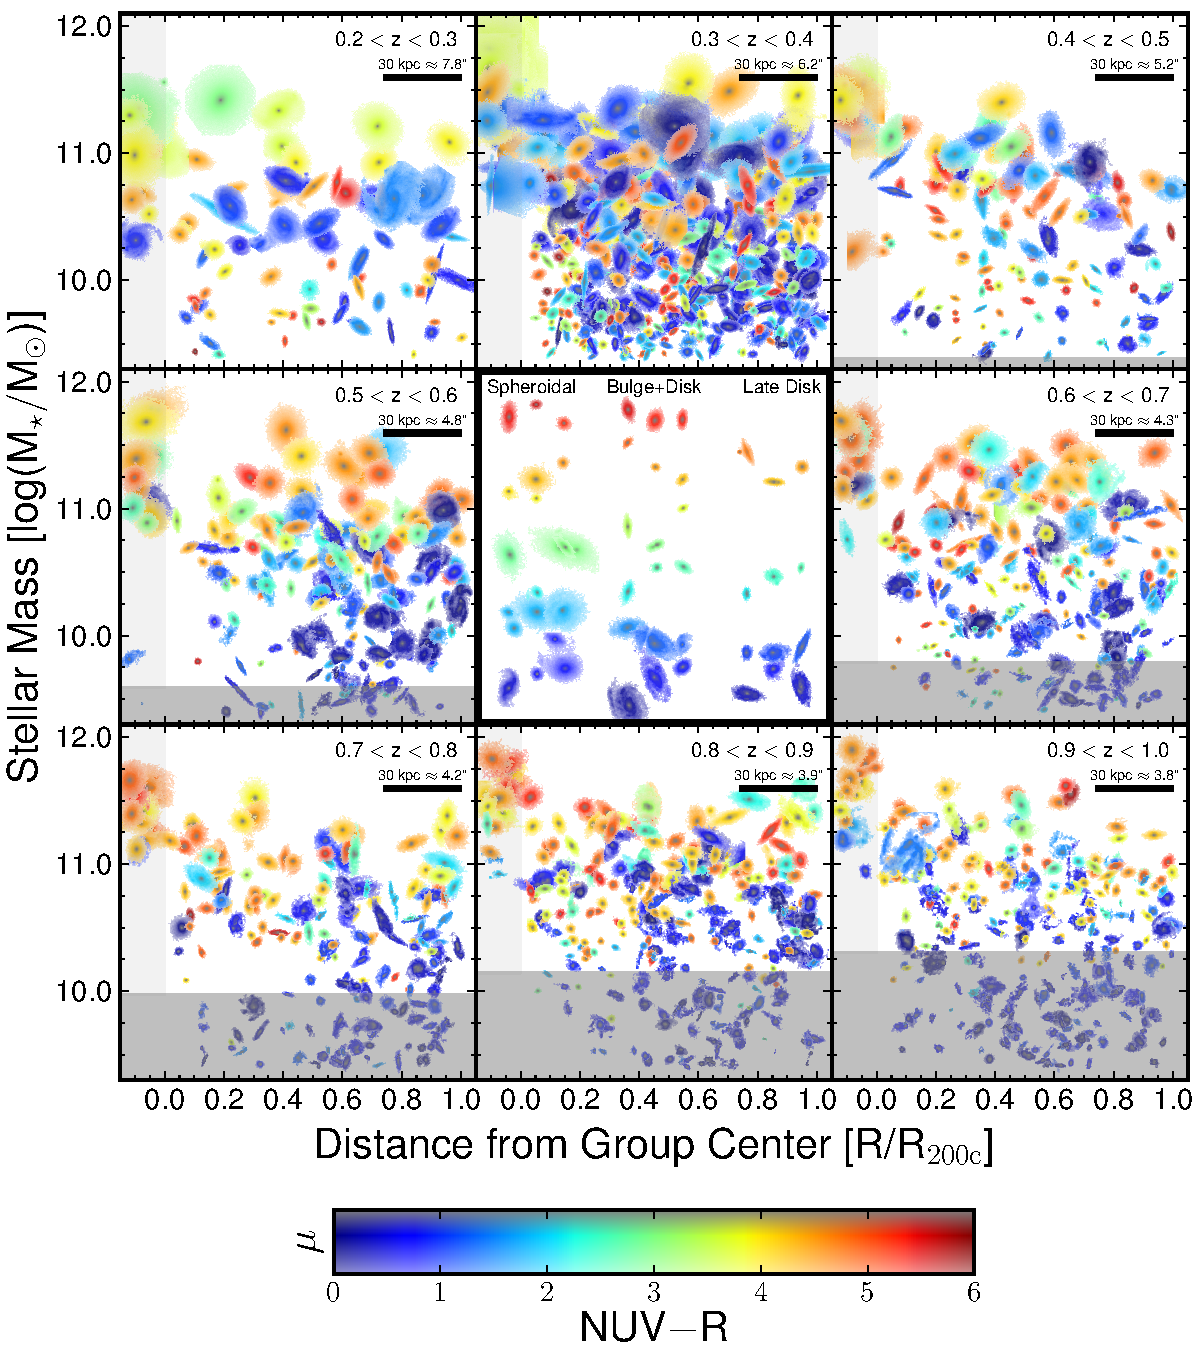
\includegraphics[scale=0.7]{transformers/fig1.pdf}
\caption{Group members as a function of stellar mass and distance from
  the group center. Colors for each galaxy represent the average
  unextincted rest-frame template \nuvr color, with shading
  proportional to the logarithmic surface brightness $\mu$. The gray
  band at the bottom of the high-redshift panels shows the stellar
  mass completeness limit for a passive population calculated with our
  flux limits F814W $ = 24.2$ and $K_s=24$ following the approach of
  \citet{Bundy2010} \citep[see also Figure 1
  of][]{George2011}. Central galaxies in these groups are shown in the
  light gray band on the left side of each of the outer panels. The
  middle frame shows morphological classifications for a random sample
  of galaxies chosen to span the range of colors observed; objects in
  this panel are sorted vertically by color and horizontal offsets
  within each classification are arbitrary.}
\label{tran_fig:candy}
\end{center}
\end{figure*}
% **** FIG *****
 
We begin our analysis with a visualization of a few properties of the
galaxies in our sample. Figure~\ref{tran_fig:candy} shows the distributions
of stellar masses and group-centric distances in different redshift
bins for all galaxies selected as group members. Each point represents
one object and is displayed using the ACS image of the galaxy \citep{Koekemoer2007}, colored
according to the average unextincted rest-frame template \nuvr
color. Centrals are positioned on the left of each panel with small
horizontal offsets, and satellites are plotted at their distance from
the corresponding central. Each image is basically the set of adjacent
pixels with flux above a noise threshold shown with a logarithmic
surface brightness scale that has its maximum set to the peak value
for each galaxy.  We note that the apparent size of a galaxy on the
plot is quite sensitive to its flux since images of brighter galaxies
have more pixels above the noise threshold, and this is not a perfect
indicator of the physical effective radius of a galaxy. A small
fraction of objects have deblending issues or edge effects from the
cutout image size, but we note that the images are processed
independently for visualization and analysis purposes.
 
Several trends are evident when visualizing galaxies in this
manner. Stellar mass is a strong determinant of galaxy properties;
massive galaxies are more likely to be large, red, and
spheroidal. Physical properties also depend on the location within a
group. Central galaxies are massive (by definition), but also
typically red and elliptical. Blue centrals tend to be less massive
than red centrals at high redshifts even within the fairly narrow
range of halo masses studied here, as discovered by
\citet{Tinker2012}. Satellites closer to group centers are more likely
to be red and show fewer spiral features than in the outskirts,
particularly at low stellar masses. There is a relative dearth of low
mass satellites near group centers; this could be a hint of satellite
depletion due to mergers, but challenges in measuring photometry of
faint objects near massive extended central galaxies could be a
contributing factor so further investigation is needed. Similar
evidence of mass segregation and the influence of mass and environment
on star formation has been seen in groups and clusters out to $z\sim
1$ \citep{Muzzin2012, Presotto2012}. Many of these trends can be seen
across the entire redshift range studied here, indicating that both
stellar mass and halo environment play a role in determining galaxy
properties at least since $z=1$. Sample variance due to the finite
survey volume does affect our ability to measure absolute redshift
trends as the number densities vary significantly due to large-scale
structures (particularly evident at $z=0.3-0.4$), but the relative
fractions of different populations should be less affected.

The central panel of Figure~\ref{tran_fig:candy} shows a few examples of
the three morphological classifications from ZEST, chosen randomly to
span the range of colors seen from redshifts $z=0.4-0.6$ and with
$\log(M_{\star}/M_{\odot})>10$. While these classifications do not
always agree with one's visual impression, there are clear differences
in structural parameters among the classes, and correlations between these automated
measurements and a galaxy's position in a group can provide an
interesting test of the dependence of morphology on environment. We
emphasize that the ZEST morphologies are correlated with, but not
identical to, traditional visual classification of ellipticals and
spirals. We compare results from multiple morphological indicators in
Section~\ref{tran_s:systematics}.

\subsection{Radial Trends: Blue Late Disks into Red Bulge+disks}
\label{tran_s:rtrends}

We can quantify some of the trends from Figure~\ref{tran_fig:candy} by
measuring the fraction of galaxies of a given color and morphology as
a function of stellar mass, group-centric distance, and
redshift. Figure~\ref{tran_fig:satrad_single} shows the fraction of
galaxies in each of the six combinations of color and morphology
categories described in Section~\ref{tran_s:otherdata}. For example, the
cyan triangles represent the fraction of galaxies in the stellar mass
and redshift range shown that are both blue and have late disk
morphology. This population makes up the majority among field galaxies
(shown at $R > R_{\rm 200c}$) but its fraction declines among
satellites, contributing less than $20\%$ of the satellite population
at $R < R_{\rm 200c}/3$. Meanwhile, the proportion of red bulge+disk
galaxies rises from $7\%$ in the field to $40\%$ among satellites in
the inner radial bin.

% **** FIG *****
\begin{figure}[htb]
\plotone{transformers/fig2.pdf}
\caption{Color and morphological fractions as a function of
  group-centric distance. These fractions are calculated for
  satellites in three equally-spaced bins out to $R_{\rm 200c}$ after
  applying contamination corrections. The field population is plotted
  to the right. Points are assigned small horizontal offsets for
  clarity. Error bars are the $1\sigma$ standard deviation of 500
  bootstrap samples. There is a clear transition from blue late disks
  dominating among field galaxies and outer satellites to red
  bulge+disks among inner satellites.}
\label{tran_fig:satrad_single}
\end{figure}
% **** FIG *****

Figure~\ref{tran_fig:satrad_single} highlights the most significant
environmental trends in our sample by focusing on low mass, low
redshift galaxies. We repeat the exercise in Figure~\ref{tran_fig:satrad}
with higher mass and redshift bins to study how these trends vary. The
broad picture is similar; blue late disks dominate in the field while
the red bulge+disk population becomes more prominent toward group
centers. Among low mass galaxies at $z>0.5$, the blue late disks
dominate everywhere, while more massive galaxies at lower redshift
have a substantial population of red spheroidals. Red late disks and
blue spheroidals do not make up a large portion of galaxies at
any mass or redshift studied. The red fraction can be determined from these plots by
  summing the three red lines, and similarly the spheroidal fraction
  is the sum of the solid lines with circular markers. The red
  fraction rises toward group centers for low mass galaxies, but is
  relatively flat among massive galaxies. We note that the abscissa for these plots is
the projected group-centric distance, and that the true radial trends measured
in spherical shells are likely more significant than observed.


% **** FIG *****
\begin{figure}[htb]
\plotone{transformers/fig3.pdf}
\caption{Color and morphological fractions of group members as a
  function of distance from the group center, for different bins of
  stellar mass (columns) and redshift (rows). Line styles and error
  bars are as defined in
  Figure~\ref{tran_fig:satrad_single}. Figure~\ref{tran_fig:satrad_single} is
  repeated in the top left panel, for comparison with weakening
  environmental trends at higher mass and redshift.}
\label{tran_fig:satrad}
\end{figure}
% **** FIG *****

\subsection{Redshift Trends}
\label{tran_s:ztrends}

Since satellites tend to fall toward halo centers, group-centric
distance is related to the timescale that galaxies have been inside
the group. The range of redshifts sampled with this data set provides
another measure of time to study evolution. Figure~\ref{tran_fig:satz} is a
transpose of Figure~\ref{tran_fig:satrad} to show the redshift trends in
the distribution of colors and morphologies. Again, there is a decline
in blue late disks among low-mass satellites near the centers of
groups, now compensated by a rise in both red spheroidals and red
bulge+disks. This trend weakens away from group centers and at
higher masses.

% **** FIG *****
\begin{figure}[htb]
\begin{center}
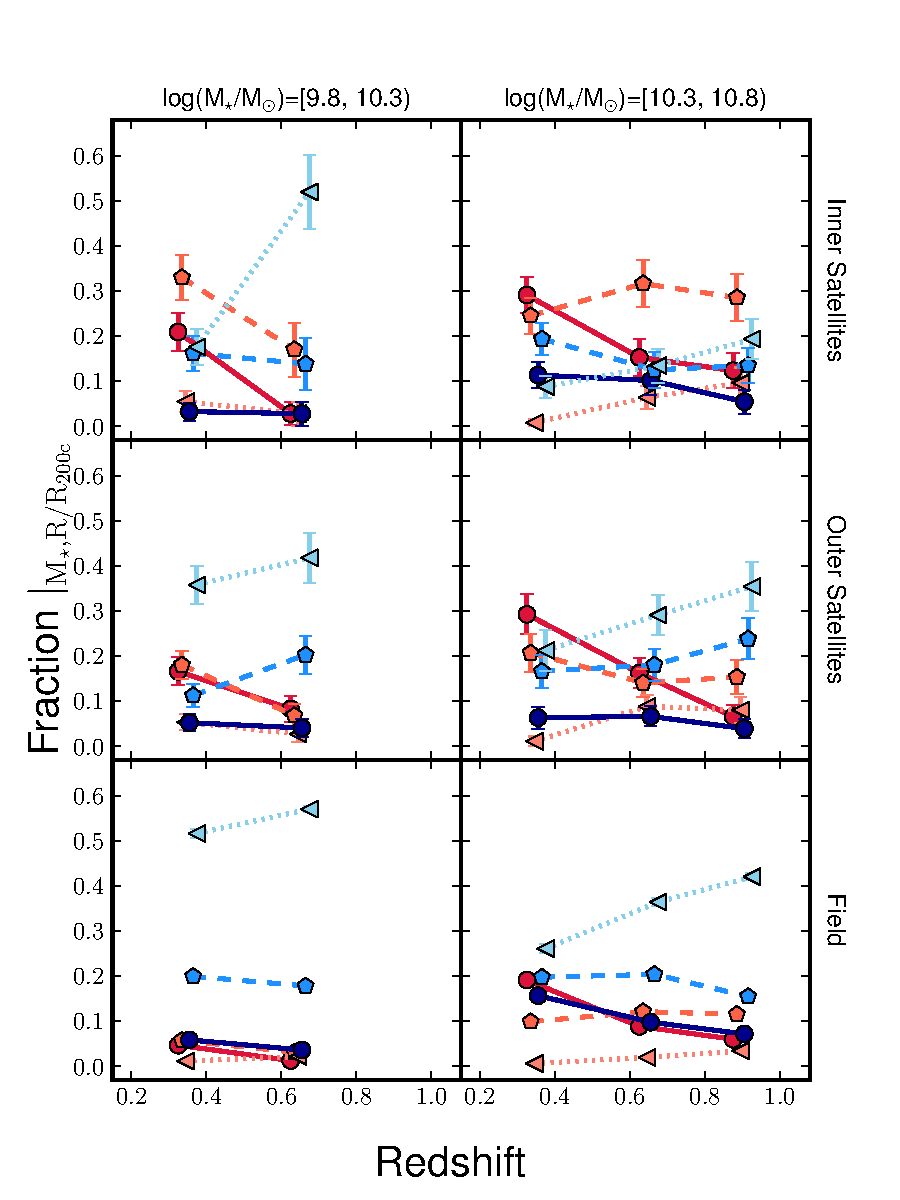
\includegraphics[scale=0.9]{transformers/fig4.pdf}
\caption{Color and morphological fractions as a function of redshift,
  for different bins of stellar mass (columns) and environment
  (rows). Inner and outer satellites are separated at a projected
  group-centric distance of $0.5 R_{\rm 200c}$. Line styles and error
  bars are as defined in Figure~\ref{tran_fig:satrad_single}.}
\label{tran_fig:satz}
\end{center}
\end{figure}
% **** FIG *****

\subsection{Checks for Systematics}
\label{tran_s:systematics}

% **** FIG *****
\begin{figure}[htb]
\plotone{transformers/fig5.pdf}
\caption{Distribution of rest-frame, extinction-corrected, template
  colors by morphological type. Galaxies from all environments are
  included. Vertical dotted lines show the cut used to segregate red
  and blue galaxies.}
\label{tran_fig:color_hist}
\end{figure}
% **** FIG *****
 
\subsubsection{Environment}

There are several possible biases or other effects in the data to
consider in order to ensure the robustness of these results. First, we
revisit the contamination of our satellite sample due to interloping
field galaxies, discussed in Section~\ref{tran_s:groupdata}. In
Figures~\ref{tran_fig:satrad_single},~\ref{tran_fig:satrad}, and~\ref{tran_fig:satz} we
have plotted values of population fractions for satellites corrected for contamination estimated
from mock catalogs. Contamination corrections are always smaller
than the statistical error bars estimated via bootstrapping, except
for low mass blue disk galaxies where it is $10\%$ greater than the
error because the field population is so large. Though the sample of satellites near $R_{\rm 200c}$ is
significantly contaminated by field galaxies, the corrections to the
relative fractions of each galaxy type are small because the field
populations are not markedly different from the outer satellites.

\subsubsection{Color Distribution}

When classifying galaxies by their spectral energy distributions (SEDs), our primary aim
is to distinguish star-forming galaxies from those that are
quenched. Though traditional indicators from emission lines or
spectral breaks are not directly available from photometry, the 31-band SEDs
used here provide a wealth of information about spectral types,
including an estimate of dust extinction that separates star-forming
galaxies that appear red due to dust from those that are truly
passive. The template-based, extinction-corrected \nuvr colors used in
this paper generally have a bimodal distribution with the color cut
from Section~\ref{tran_s:otherdata} falling on the red end of the ``green
valley.'' The color distributions for different morphological types
are shown in Figure~\ref{tran_fig:color_hist}. Shifting the cut slightly in
either direction shifts the amplitude of the red fraction in
Figures~\ref{tran_fig:satrad_single},~\ref{tran_fig:satrad}, and~\ref{tran_fig:satz}
up or down, but the trends with group-centric distance and redshift do
not vary significantly. We have tested an alternative ``red sequence''
selection suggested by \citet{Ilbert2010}, ${\rm NUV - r^+} >
0.5\log(M_{\star}/M_{\odot}) - 0.8 z - 0.5$, using rest-frame absolute
magnitudes but applying no extinction correction. The transformation
of blue late disks into red bulge+disks among low mass satellites is
still evident. Similarly, applying the two-color cut in the ${\rm NUV
  - r^+}$, ${\rm r^+ - J}$ plane used by \citet{Bundy2010} does not
qualitatively change our results.

\subsubsection{Morphologies}
\label{tran_s:sys_morph}

Morphological classification is a challenging problem and significant
scatter exists between the types assigned to galaxies in both visual
and automated analyses. In general, visual analyses emphasize the
presence or absence of spiral features, categorizing objects as
spirals or ellipticals, often with an intermediate class of S0s
grouped with ellipticals. Automated analyses measure structural
parameters such as concentration and asymmetry which are then
generally tied to a training set of visual classifications. The
correlation between the properties measured is imperfect, so we test
the impact on our results of using a variety of automated
morphological classifications, all based on the ACS F814W imaging. The
alternative classifications come from \citet{Tasca2009}, which
presented three separate techniques.

The differences between the results of each catalog and those from the
ZEST classification used in this paper are driven by how bulge+disk
galaxies are classified, since the other catalogs do not split the
spiral/disk category into multiple bins as ZEST does. For instance,
among the $237$ satellites used for Figure~\ref{tran_fig:satrad_single},
the ZEST classifications are $22\%$ spheroidal, $36\%$ bulge+disk,
$37\%$ late disk, and $5\%$ irregular or unclassified. The three separate
classifications for these galaxies from \citet{Tasca2009} vary between
$39 - 59\%$ E/S0s and $59 - 40\%$ spirals.
When bulge+disk galaxies are mostly classified as E/S0s, the
spheroidal populations (both blue and red) in Figures~\ref{tran_fig:satrad}
and~\ref{tran_fig:satz} are significantly elevated but show similar trends
with group-centric distance and redshift. In the opposite case where
bulge+disk galaxies are mostly treated as disks, the spheroidal
fraction is essentially unchanged. While the dominant population in
each panel of Figure~\ref{tran_fig:satrad} and~\ref{tran_fig:satz} can change
depending on which category the intermediate bulge+disk galaxies fall
into, the radial trend in low mass satellites is unchanged; the blue
late type fraction declines toward group centers and is compensated
with a rise in red early types. The redshift trend for this transition
is strongest for low mass satellites near group centers and weakens
toward larger radii and stellar masses. Though the scatter between
morphological classifications signals that our results should be
interpreted and compared to others with caution, the significant
trends with group-centric distance and redshift for the intermediate
bulge+disk galaxies suggests that the ZEST classification has
identified a population in transition.

\subsubsection{A Population of Blue Spheroidals}

While the tests described above suggest that our measures of
environment, color, and morphology are robust, we do note a puzzling
population of massive blue spheroidals that can be seen most clearly
in the bottom right panel of Figure~\ref{tran_fig:satz} as well as the
right column of Figure~\ref{tran_fig:color_hist}. Those plots suggests
that half of all spheroidals in that stellar mass range are blue,
exceeding measurements in other studies \citep[e.g.][]{Kaviraj2007,
  Kaviraj2008, Bamford2009, Schawinksi2009, Ilbert2010}, but see also
\citet{Cross2004} who found a large fraction of blue ellipticals in a
luminosity-selected sample at moderate redshift. We see a similarly
large blue fraction among spheroidals at higher masses
($\log(M_{\star}/M_{\odot}) > 10.8$, not plotted) where spheroidals make up a
higher proportion of all galaxies, and most prominently at low
redshift ($z<0.5$). Visual inspection of the ACS images of these
galaxies suggest that $30-40\%$ show spiral or irregular features,
although the structural parameters measured by the automated
classifiers are all consistent with the red spheroidal population. We
have also investigated the UV-optical and optical-IR colors of these
massive blue spheroidals prior to template fitting, in addition to
optical spectra for $30$ of these objects described in
\citet{George2011}. These data suggest that blue spheroidals are not
typical star-forming galaxies but may have a small amount of recent
star formation to which rest-frame UV measurements are particularly
sensitive \citep[e.g.][]{Kaviraj2007, Kaviraj2008}. Another possible
explanation is that there are unusual stellar populations that are not
represented in the template fits used to derive our \nuvr colors
\citep[see e.g.][for a discussion of galaxy properties contributing to
the ``UV upturn'']{Smith2012}. While this population is interesting in
its own right, it is most prominent at high stellar masses and does
not show a strong dependence on environment, so we do not consider it
further here.

\section{Discussion and Conclusions}
\label{tran_s:discussion}

Our results indicate a complex relationship between color, morphology,
stellar mass, and group-centric distance. Trends in color and
morphology are distinct, and the use of a single property as proxy for
galaxy type does not capture the whole picture. The most interesting
trend seen is the shift in dominance among the low mass population
from blue late disk galaxies in the outskirts to red bulge+disk types
in group interiors. If part of one population was merely disappearing
from the sample, either due to changes in mass or merging with other
galaxies, then the other populations would all be expected to grow by
an equal factor. The fact that the decline in one population is
roughly balanced by the rise of a single other population suggests a
transformation process. We now discuss these results in the context of
past analyses, the physical implications of the present work, and
future avenues to clarify the role of environment in galaxy evolution.

\subsection{Connection to Previous Observations}

There is a long history of research into the covariance between the
stellar masses, colors, morphologies, and environments of galaxies and
its evolution with time. After controlling for differences in stellar
mass or luminosity, numerous studies at low redshift have found that color is more
strongly correlated with environment than morphology
\citep[e.g.,][]{Kauffmann2004, Blanton2005, Christlein2005, vandenBosch2008,
  Bamford2009, Skibba2009, Weinmann2009}. The implication of these
studies is that the well-known correlation between morphology and
environment is secondary to correlations between morphology and
stellar mass or color, with the latter properties more physically
linked to environment. Still, some of these studies find residual
correlations between morphology and environment after controlling for
color and stellar mass or luminosity, particularly at low masses and
among late to intermediate morphologies \citep{Blanton2005,
  Weinmann2009, Skibba2012}.

Moving from large low-redshift studies to moderate redshifts ($z\sim0.4$), \citet{Balogh2009} and
\citet{McGee2011} have shown that groups still host a higher fraction of red
galaxies than the field, while \citet{Wilman2009} found
an elevated S0 fraction in groups with a mildly significant rise with
group-centric distance. This radial trend in morphology is the opposite of that seen
in Figure~\ref{tran_fig:satrad} but may be due to a smaller sample size or
the use of luminosity-weighted centroids, which have been shown to be
a poorer tracer of halo centers measured by weak lensing when compared
with the most massive galaxy used in this catalog \citep{George2012}.

Environmental trends at fixed stellar mass have been seen to weaken at
higher redshift \citep[e.g.,][]{Poggianti2008, Tasca2009,
  Cucciati2010, Iovino2010, Kovac2010b}, though recent analyses have
shown clear differences between the fraction of star-forming galaxies
across environments over a range of stellar masses at least up to $z\sim1$
\citep{Cooper2010, Peng2010, George2011, Knobel2012}. \citet{Tasca2009} and
\citet{Kovac2010b} have compared the dependence of colors and
morphologies on local density and in groups in the COSMOS field,
finding a stronger effect on color than on morphology, similar to the
low redshift results and suggesting a longer timescale for structural
transformations than for quenching star-formation. \citet{Muzzin2012}
and \citet{Presotto2012} have also shown that the quenched fraction
among satellites depends significantly on group-centric distance at
these redshifts.

The results presented here extend this work to include radial trends
in colors and morphologies from $z=0.2-1$. Our X-ray group catalog
gives a large, clean, and fairly representative selection of
$10^{13}-10^{14}~{\rm M_{\odot}}$ halos \citep{Finoguenov2010}, and
has been well-calibrated based on 
its weak lensing signal \citep{Leauthaud2010, George2012}. We detect significant
trends in both color and morphology with group-centric distance. Some previous studies measured weak or insignificant
gradients in morphology by using a simple dichotomy of spirals and
ellipticals, and we can reproduce these results when using a coarse
morphological binning (see discussion in Section~\ref{tran_s:sys_morph}). But in contrast
to those results, we see clear morphological gradients at
fixed stellar mass and color once the morphological classification
considers differences in the bulge content of disk galaxies.

The importance of this intermediate morphology between pure disks and
spheroidals has been noted before in the context of S0 galaxies which
have been known to dominate the evolution in the morphology-density
relation \citep{Dressler1997, Postman2005, Smith2005a, Boselli2006b,
  Moran2007, Oesch2010, Lackner2013}.
\citet{Smith2005a} also showed that morphological evolution occurs
later in less dense regions than in the densest regions associated
with clusters, with little evolution at intermediate densities from
$z=1$ to $0.5$ followed by an increase in early types at lower
redshift. There is a significant overlap between the intermediate
bulge+disk population in our analysis and visually classified S0
galaxies although these bulge+disk galaxies are often classified
slightly later along the Hubble sequence \citep{Scarlata2007}. Our
results in Figure~\ref{tran_fig:satz} broadly corroborate those of
\citet{Smith2005a} and add that color and stellar mass are also
important dimensions when studying these trends.

\subsection{Implications for Physical Mechanisms of Galaxy Transformation}

The radial gradients and redshift trends measured in
Section~\ref{tran_s:results} suggest a transformation among low mass
satellites from blue late disks into red bulge+disks and spheroidals.
The mechanism for this transformation must affect both color and
morphology, or more physically, the star formation rate and stellar
kinematics. Some processes \citep[see e.g.][for a review]{Boselli2006}
halt star formation without significantly altering stellar structure,
such as gas removal via ram pressure stripping or weak tidal
interactions, suppression of gas accretion within dense
shock-heated environments, or quasar feedback. On the other hand, galaxy mergers and
strong tidal interactions can affect both the distribution of gas
needed to form stars as well as the stellar morphology. A third
possibility is that color and morphology changes are physically
coupled; bulge growth could stabilize a galaxy against
  disk fragmentation and suppress star formation \citep{Martig2009},
  or gas loss may leave a disk unable to dissipate energy from tidal
  interactions or may drive instabilities leading to bulge growth.
Yet another scenario is that a bulge only appears more prominent after
a galaxy is quenched because the previously star-forming disk has
faded.

We can test these models by studying the morphological dependence on
environment among quenched galaxies. Mechanisms like gas stripping or
disk fading that do not directly affect morphology should produce a
higher fraction of quenched galaxies in dense environments, but among
quenched galaxies the morphological distribution should be
constant across environments. On the other hand, if quenched galaxies in dense
environments have more bulge-dominated morphologies than quenched
field galaxies, it would suggest that mergers or strong tidal
interactions altering the structure of galaxies occur in addition to,
or in conjunction with, the suppression of star formation. The results
of this test are plotted in Figure~\ref{tran_fig:satradred}, where we show
the fractions of red galaxies that are early and late type as a
function of environment. We have used a broad redshift range and
combined the spheroidal and bulge+disk categories to reduce
statistical errors for this smaller population of red
galaxies. Figure~\ref{tran_fig:satradred} demonstrates that quenched
satellites, particularly those in the inner regions of groups, are
more likely to be bulge-dominated than their field
counterparts. 

We interpret this to mean that some physical process in dense
environments is driving bulge growth. Though some field studies \citep{Bundy2010, Masters2010}
have already noted a tendency of passive disks to be more concentrated than
star-forming disks, we find that the morphological evolution of
quenched galaxies is even stronger in groups. Our result is consistent with previous
arguments favoring bulge growth over disk fading based on the higher
typical luminosities of galaxies with intermediate morphologies
compared to late types \citep{Christlein2004,Burstein2005}. The data
presented here show that even at fixed mass there must be bulge enhancement
that accompanies quenching in groups.

% **** FIG *****
\begin{figure}[htb]
\plotone{transformers/fig6.pdf}
\caption{Morphological fractions \textit{among red galaxies} as a
  function of distance from the group center. The small but
  significant excess in early-type morphologies among inner satellites
  relative to field galaxies suggests that mergers or tidal
  interactions cause more significant bulge growth among
  satellites.}
\label{tran_fig:satradred}
\end{figure}
% **** FIG *****

% **** FIG *****
\begin{figure*}[htb]
\plottwo{transformers/fig7a.pdf}{transformers/fig7b.pdf}
\caption{Illustrations of our main results and interpretation. Left
  panel shows the projected positions of satellites in an ensemble
  group with the same stellar mass and redshift range as
  Figure~\ref{tran_fig:satrad_single} with only the blue late disks (which
  dominate the outskirts) and red bulge+disks (which dominate the
  interior) displayed. The schematic diagram at right shows the effects of various
  physical mechanisms on color and morphology; the large arrow
  indicates the observed transformation from blue late disks to red
  bulge+disks, suggesting a combination of processes.}
\label{tran_fig:cartoons}
\end{figure*}
% **** FIG *****

The results of Figure~\ref{tran_fig:satrad} suggest that the timescale for
the morphological transition from late disk to bulge+disk must be
comparable to the timescale for quenching in order to turn blue late
disks directly into red bulge+disk galaxies. For example, if quenching
occurred via gas stripping or removal at a rate faster than any
structural changes, we would expect to see blue late disks turning
into red late disks. Instead we observe a growth in red galaxies with
earlier morphologies whenever blue late disks decline.  The fraction
of blue late disks plummets by more than a factor of two in
$\sim2~{\rm Gyr}$ among inner satellites (top left panel of
Figure~\ref{tran_fig:satz}), while the fraction of red late disks is nearly
constant and the fraction of red bulge+disks grows. Similarly, we do
not detect a large population of blue bulge+disk galaxies which might
be expected if bulge growth happened faster than quenching. These
observations suggest that some morphological evolution occurs on a
similar timescale as quenching.

At the same time, the morphological transformation observed at low
stellar masses has not fully turned many disks into spheroidals. The
bulge+disk galaxies are still categorized as disks in the top level
ZEST classification.  This echoes earlier results finding a buildup of
S0s in clusters but weaker evolution in the relative abundance of
ellipticals \citep[e.g.,][]{Dressler1997}. Though the fraction of red
spheroidals does not correlate significantly with group-centric
distance (Figure~\ref{tran_fig:satrad}), it does grow globally with time
(Figure~\ref{tran_fig:satz}). This may indicate that different processes
are responsible for producing bulge+disks and spheroidals. 

The discreteness of morphological classification makes detailed
comparison of transformations in morphology and color somewhat
difficult, but the structural evolution appears to contrast with that
in color, where a clear bimodality separates red and blue states and
the relatively low intermediate population suggests a fast quenching
timescale once it begins (e.g., \citealt{Wetzel2012a}, though see
\citealt{Balogh2011}). One could test the hypothesis that galaxies pass through an
intermediate state between blue late disk and red bulge+disk by
measuring the time since quenching based on the SEDs of galaxies in
these intermediate states. Is there a difference in the mean color of
blue bulge+disks and blue late disks, or between red bulge+disks and
red late disks? Figure~\ref{tran_fig:color_hist} does not show conclusive
differences in the colors of these populations, and the satellite
sample size is too small to constrain differences in the distribution
of colors within the red and blue populations. More detailed analysis
with spectroscopic data could better constrain such evolutionary
models.

The group environment can play an important role in building up the
well-studied color-morphology-density relations in nearby clusters. A
group of mass $10^{13.5} M_{\odot}$ at $z=1$ should grow through
mergers by an average of $0.3$ dex to $z=0$ \citep{Fakhouri2010}, so
some of our high redshift groups will be the progenitors of massive
clusters and others may accrete onto them. For comparison, a typical
star-forming galaxy should grow by $0.2$ dex in stellar mass between
each of our three redshift bins and by $0.7$ dex from $z=1$ to $0$
\citep{Elbaz2011}.  \citet{Wetzel2012b} show that the dominant
population of satellites in the most massive halos at $z=0$ were
already satellites in groups when accreted. Our results demonstrate
that both the color and morphology of these satellites are influenced
in the group environment, showing the importance of ``preprocessing''
of galaxies prior to entering massive clusters. The bulge+disk
population we see here is not quite as morphologically evolved as the
growing S0 population seen at low redshift and in massive clusters,
but likely precedes it.
 
We summarize our main results and interpretation in
  Figure~\ref{tran_fig:cartoons}. The left panel shows the positions of
  satellites for a stacked group and highlights the trend in
  Figure~\ref{tran_fig:satrad_single} with blue late disks dominating the
  outskirts and red bulge+disk galaxies making up most of the inner
  satellite population. This combination of color and morphology
  transformations suggests some combination of gas removal and bulge
  growth, shown in the right panel. While the diagram is a
  simplification of a wide variety of model predictions, the primary
  point is that \textit{both} color and morphology are affected in
  group satellites, so physical mechanisms that explain environmental
  correlations should reflect this.

\subsection{Future Prospects}

While these measurements add insight to the transformation of galaxy
properties, much work remains to be done to constrain the variety of
physical mechanisms that may be responsible. A cleaner bulge-disk
decomposition would be useful to track the growth of bulges and the
importance of disk fading \citep[e.g.,][]{Lackner2012,
  Lackner2013}. Incorporating the physical sizes of each component
would also help to link these transformations with the significant
growth seen in early types since $z\sim2$
\citep[e.g.,][]{Bruce2012}. With deep high-resolution imaging from
\textit{HST}, the CANDELS survey \citep{Grogin2011,Koekemoer2011} is pushing these
studies to higher redshift and should also allow bulge-disk
decomposition to be studied at multiple wavelengths, identifying when
and where star formation is happening or stopping. Alternatively,
visual classifications from an ongoing Galaxy Zoo project in the
CANDELS fields will track the evolution of spiral features and bars
which are challenging for automated techniques. Impending wide field
imaging surveys will add greatly to the statistics of these analyses.

Different measures of environment may also help disentangle the
relevant physical mechanisms. While we have argued in favor of
halo-based indicators (see \citealt{George2011} for a discussion), the
local galaxy density \textit{within a halo}, in addition to
group-centric distance, may shed light on galaxy-galaxy interactions
and infalling substructure \citep[e.g.,][]{Blanton2007, Cibinel2012b,
  Woo2012}. However, this indicator is a noisy quantity affected by
shot noise, redshift errors, and peculiar velocities, likely
requiring deep and complete spectroscopic data for clean
results. Larger surveys will also enable a wider range of halo masses
to be probed at higher redshift. Comparison of different halo mass
proxies can provide a test of environmental mechanisms, for example if
X-ray bright groups are more efficient at ram pressure stripping
satellites than groups with less hot gas.

These studies can also be extended to the interplay of environmental
mechanisms with non-stellar components of galaxies, namely the gas
content and central black holes in galaxies. Current and planned radio
arrays will extend the study of neutral and molecular gas beyond the
local Universe allowing a clearer picture of how star-formation is fed and
quenched. And the growth of bulges seen in this paper should be
connected with accretion onto the central black hole in order to
explain the tight correlation seen locally between these components.

Finally, while we have simply presented an empirical description of
the data here, we can extend this work by modeling the evolution of
color and morphology with environment. \citet{Peng2010} and
\citet{Wetzel2012b} present simple empirical descriptions of the
fraction of quenched galaxies as a function of stellar mass and
environment. Incorporating morphologies into this framework will
further illuminate the physical processes at work that build up the
environmental correlations we observe.

\chapter{Pecular Velocities}

\label{chap:flow}

%-------- ABSTRACT  ---------------------
  
 
%--------------------------------------------------------------
% INTRODUCTION
%--------------------------------------------------------------

\section{Introduction}


\section{Data and Mocks}
\label{flow_s:data}

\section{Fitting the Fundamental Plane}

\section{Velocity Correlations}

\section{Prospects}

\chapter{Spectroscopic Weak Lensing}

\label{chap:speclens}

%-------- ABSTRACT  ---------------------
  
 
%--------------------------------------------------------------
% INTRODUCTION
%--------------------------------------------------------------

\section{Introduction}

We explore a technique first described by \citet{Blain2002} and
further elucidated by \citet{Morales2006} to use distortions in
measured velocity maps of galaxies as a probe of weak lensing by
foreground structure. Traditional weak lensing measurements seek to
constrain the shear induced on galaxy images and are limited by the
fact that galaxies have a broad range of intrinsic shapes and only the
lensed shapes are observed. Measurement of the velocity field of stars
or gas in the source galaxy can provide information about the
intrinsic shape and orientation of the galaxy, with a potential for
dramatically reducing the intrinsic shape noise. Such a measurement
translates into a great improvement of signal to noise for a given
lensing survey, or alternatively, allows for a modified survey
strategy with fewer source galaxies to achieve a given signal to
noise. An additional benefit to this approach is that potential
systematic errors are very different from traditional shear
measurements, providing cross-checks for possible biases due to errors
in photometric redshifts or shape measurements for example.

This work extends that of \citet{Blain2002} and \citet{Morales2006} by
incorporating the Tully-Fisher \citep{Tully1977} relation as a prior
on the amplitude of the velocity field which enables tighter
constraints on the intrinsic shapes of galaxies with limited data. We
also present a survey strategy using dithered pointings of a
multi-object optical spectrograph to coarsely map the velocity fields
of many galaxies simultaneously.

\section{The Idea}

Outline the principle of measuring velocity fields, incorporating TF
relation, inferring shapes and shears with velocity field only /
velocity field plus imaging.

% **** FIG *****
\begin{figure*}[htb]
%\epsscale{1.2}
\plottwo{speclens/fig1a}{speclens/fig1b}
\caption{Velocity maps for a galaxy with $PA=20\degr, b/a=0.3$. Left is unsheared, right is sheared $(e1,e2)=(0,0.3)$.}
\label{speclens_fig:vmap}
\end{figure*}
% **** FIG *****
 

\section{Simulations}

Galaxy image, PSF, shear, velocity maps, fiber integration.

Fitting models to observables.

% **** FIG *****
\begin{figure*}[htb]
%\epsscale{1.2}
\plottwo{speclens/fig2a}{speclens/fig2b}
\caption{Image (left) and flux-weighted, PSF-convolved velocity map
  (right) for a galaxy with $PA=20\degr, b/a=0.3$ and Gaussian seeing
  with $\rm{FWHM}=1.5\arcsec$. The overlaid circles show a 7-point dither
  pattern of fibers with radius $1\arcsec$.}
\label{speclens_fig:fiber_pattern}
\end{figure*}
% **** FIG *****

% **** FIG *****
\begin{figure*}[htb]
%\epsscale{1.2}
\plotone{speclens/fig3}
\caption{Line of sight velocity in a ring of radius $2\arcsec$
  corresponding to the centers of the outer fiber positions shown in
  Figure~\ref{speclens_fig:fiber_pattern}. Model parameters are those shown in
  the legend, with a fiducial model followed by other models with one
  parameter altered. Error bars show expected velocity uncertainties
  ($30~{\rm km/s}$) measured at the positions of the six outer fibers.}
\label{speclens_fig:observable}
\end{figure*}
% **** FIG *****


\section{Survey Plan}

Flux limit, sample density, estimated S/N.

Cluster field, galaxy-galaxy lensing, cosmic shear??

Based on GalSim package\footnote{Available at \url{https://github.com/GalSim-developers/GalSim}}

\section{Caveats}

Intrinsic disk ellipticity (see \citealt{Franx1992, Franx1994}), OII
distribution, uncertain velocity profiles, uncertain TF evolution, PSF
variation across pointings.

















\section{Shear and Galaxy Kinematics}
\label{speclens_s:theory}

\section{Observational Effects}

\section{Prospects}

\bibliography{thesis}{}
\end{document}
